\documentclass{article}


% if you need to pass options to natbib, use, e.g.:
%     \PassOptionsToPackage{numbers, compress}{natbib}
% before loading neurips_2025


% ready for submission
\usepackage{neurips_2025}


% to compile a preprint version, e.g., for submission to arXiv, add add the
% [preprint] option:
%     \usepackage[preprint]{neurips_2025}


% to compile a camera-ready version, add the [final] option, e.g.:
%     \usepackage[final]{neurips_2025}


% to avoid loading the natbib package, add option nonatbib:
%    \usepackage[nonatbib]{neurips_2025}
\usepackage{enumitem}
% Recommended, but optional, packages for figures and better typesetting:
\usepackage{microtype}
\usepackage{graphicx}
\usepackage{subcaption}
\usepackage{adjustbox}
\usepackage{multirow}
\usepackage{placeins}  % Add this in the preamble
\usepackage{float}
\usepackage{booktabs} % for professional tables
\usepackage{etoolbox}
\patchcmd{\quote}{\rightmargin}{\leftmargin 0.2em \rightmargin}{}{}



% hyperref makes hyperlinks in the resulting PDF.
% If your build breaks (sometimes temporarily if a hyperlink spans a page)
% please comment out the following usepackage line and replace
% \usepackage{icml2025} with \usepackage[nohyperref]{icml2025} above.
% For theorems and such
\usepackage{amsmath}
\usepackage{amssymb}
\usepackage{mathtools}
\usepackage{amsthm}
\usepackage{wrapfig}
\usepackage{enumitem,makecell}
\usepackage[skins]{tcolorbox} % for little color boxes
\newcommand{\best}[1]{\colorbox{black!10}{#1}}
\definecolor{valbest}{HTML}{d9ead3}
\newcommand{\valbest}[1]{\colorbox{valbest}{#1}}
\definecolor{valgood}{HTML}{cfe6ec}
\newcommand{\valgood}[1]{\colorbox{valgood}{#1}}
\definecolor{valmid}{HTML}{fce5cd}
\newcommand{\valmid}[1]{\colorbox{valmid}{#1}}
\definecolor{valbad}{HTML}{ead1dc}
\definecolor{llamiabench}{HTML}{D8D4F2}
\newcommand{\llamiabench}[1]{\colorbox{llamiabench}{#1}}
\newcommand{\valbad}[1]{\colorbox{valbad}{#1}}
\definecolor{themegreen}{HTML}{365956}
\definecolor{themepurple}{HTML}{3c1b48}
\definecolor{themered}{HTML}{b43748}
\newcommand{\somesh}[1]{\textcolor{red}{[Somesh: #1]}}
\definecolor{themeharini}{RGB}{50,128,128}
\newcommand{\harini}[1]{\textcolor{themeharini}{[Harini: #1]}}

\definecolor{yamanColor}{RGB}{0, 128, 255}
\newcommand{\yaman}[1]{\textcolor{yamanColor}{\scriptsize \textit{#1}}}


\newcommand{\yaman}[1]{{\scriptsize\textcolor{red}{[Yaman: #1]}}}

%%%%%%%%%%%%%%%%%%%%%%%%%%%%%%%%
% THEOREMS
%%%%%%%%%%%%%%%%%%%%%%%%%%%%%%%%
\theoremstyle{plain}
\newtheorem{theorem}{Theorem}[section]
\newtheorem{proposition}[theorem]{Proposition}
\newtheorem{lemma}[theorem]{Lemma}
\newtheorem{corollary}[theorem]{Corollary}
\theoremstyle{definition}
\newtheorem{definition}[theorem]{Definition}
\newtheorem{assumption}[theorem]{Assumption}
\theoremstyle{remark}
\newtheorem{remark}[theorem]{Remark}
\input{math_commands.tex}
% Todonotes is useful during development; simply uncomment the next line
%    and comment out the line below the next line to turn off comments
%\usepackage[disable,textsize=tiny]{todonotes}
\usepackage[textsize=tiny]{todonotes}


% Attempt to make hyperref and algorithmic work together better:
\newcommand{\theHalgorithm}{\arabic{algorithm}}


\usepackage[utf8]{inputenc} % allow utf-8 input
\usepackage[T1]{fontenc}    % use 8-bit T1 fonts
\usepackage{hyperref}       % hyperlinks
\usepackage{url}            % simple URL typesetting
\usepackage{booktabs}       % professional-quality tables
\usepackage{amsfonts}       % blackboard math symbols
\usepackage{nicefrac}       % compact symbols for 1/2, etc.
\usepackage{microtype}      % microtypography
\usepackage{xcolor}         % colors
\usepackage[capitalize,noabbrev]{cleveref}

\renewcommand{\arraystretch}{0.95}

\title{LLAMIA: Large Language and Action Models with Internal Agents for Decision Making and Reasoning}


% The \author macro works with any number of authors. There are two commands
% used to separate the names and addresses of multiple authors: \And and \AND.
%
% Using \And between authors leaves it to LaTeX to determine where to break the
% lines. Using \AND forces a line break at that point. So, if LaTeX puts 3 of 4
% authors names on the first line, and the last on the second line, try using
% \AND instead of \And before the third author name.


\author{%
  David S.~Hippocampus\thanks{Use footnote for providing further information
    about author (webpage, alternative address)---\emph{not} for acknowledging
    funding agencies.} \\
  Department of Computer Science\\
  Cranberry-Lemon University\\
  Pittsburgh, PA 15213 \\
  \texttt{hippo@cs.cranberry-lemon.edu} \\
  % examples of more authors
  % \And
  % Coauthor \\
  % Affiliation \\
  % Address \\
  % \texttt{email} \\
  % \AND
  % Coauthor \\
  % Affiliation \\
  % Address \\
  % \texttt{email} \\
  % \And
  % Coauthor \\
  % Affiliation \\
  % Address \\
  % \texttt{email} \\
  % \And
  % Coauthor \\
  % Affiliation \\
  % Address \\
  % \texttt{email} \\
}


\begin{document}


\maketitle


\begin{abstract}
Foundation models (FMs) exhibit strong zero-shot generalization in language (e.g., BERT, GPT-3) and vision (e.g., ViTs) across downstream tasks. Building on this, recent research has explored the use of Large Language Models (LLMs) as general-purpose planners for agentic systems in domains such as gaming, marketing, virtual assistants, and autonomous driving. However, despite their extensive world knowledge, LLMs continue to struggle with structured, multi-step reasoning and long-horizon planning. We introduce LLAMIA, a novel framework that integrates pretrained domain-specific agents into LLMs by projecting latent agent states directly into the LLM’s token space. This allows LLMs to internalize and invoke agent behavior autoregressively, augmenting their intrinsic planning and reasoning capabilities.
Paired with Lc0, a chess engine, LLAMIA models based on Vicuna (7B, 13B) achieve grandmaster-level performance without search. They outperform fine-tuned experts, significantly larger LLMs (e.g., GPT-4o, LLaMA-3 405B), and tool-augmented systems across planning and reasoning tasks including behavior cloning ($\uparrow$5–10\%), commentary generation ($\uparrow$20–25\% BLEU), and conditional planning ($\uparrow$7–10\% win rate). We further demonstrate LLAMIA's extensibility to other environments (1) Text-to-Image preference alignment, improving over VisionReward by +7.9\% win rate in DPO and 5\% in preference prediction accuracy (2) Persuasion Modeling, $\sim$5\% improvement in persuasion prediction. These results also highlight LLAMIA’s robustness and its potential to generalize across perceptual and behavioral environments.
\vspace{-5mm}
\end{abstract}
\begin{figure}[!h]
    \centering
    \begin{subfigure}[b]{0.3\linewidth}
        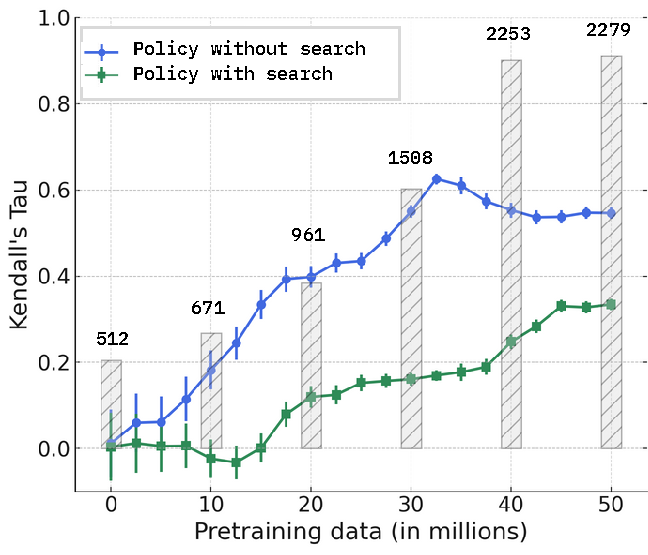
\includegraphics[width=\linewidth]{kt1.pdf}
        \caption{Policy alignment improves with projector pretraining data scale. LLAMIA approaches search-quality behavior, indicating internal lookahead of depth 4.}
      
        \label{fig:kt}
    \end{subfigure}
    \hfill
    \vspace{5mm}
    \begin{subfigure}[b]{0.32\linewidth}
    \vspace{-3mm}
        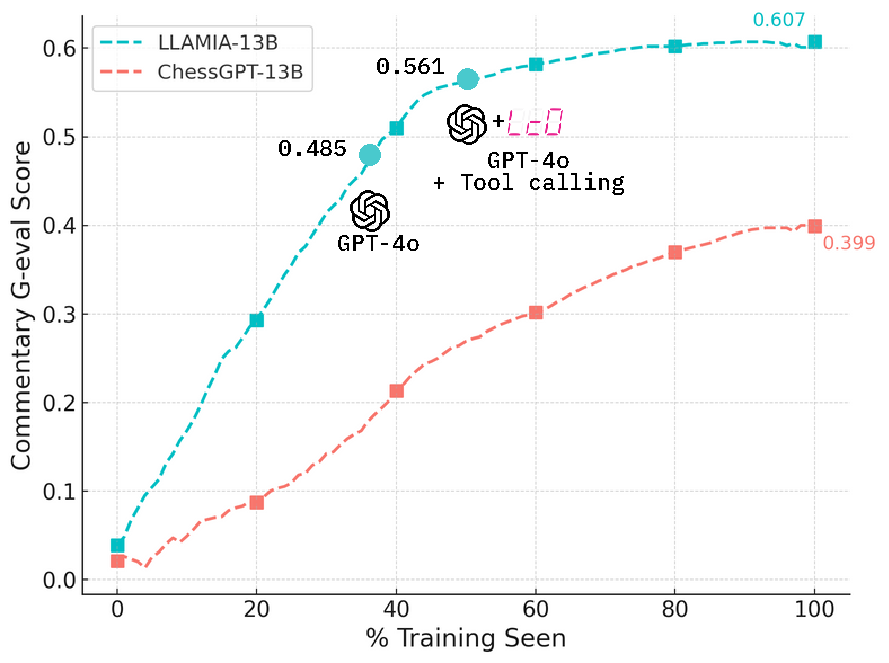
\includegraphics[width=\linewidth]{comm.pdf}
        \caption{Stage-2 training data scale vs. game-level commentary generation. LLAMIA matches GPT-4o + tool calling performance using only 50\% of the data, showing strong data efficiency.}
        \label{fig:commentary}
        
    \end{subfigure}
    \hfill
    \begin{subfigure}[b]{0.32\linewidth}
        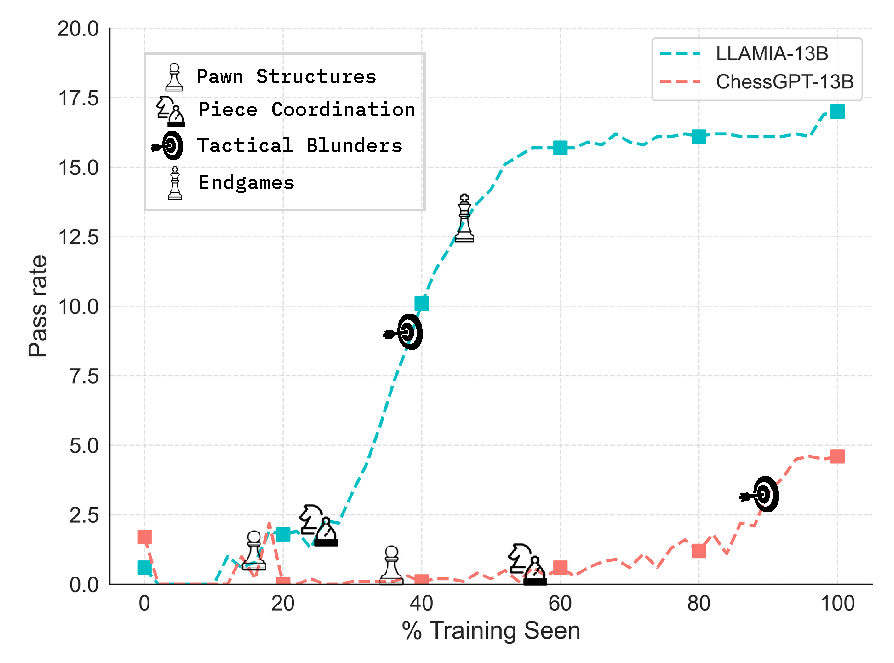
\includegraphics[width=\linewidth]{icp.pdf}
        \caption{Stage-2 training scale vs. conditional planning. LLAMIA acquires targeted weaknesses (icons show skill acquisition) with significantly fewer training examples.}
        \label{fig:icp}
        
    \end{subfigure}
    \caption{LLAMIA shows consistent improvement over instruction fine-tuning (IFT) with tool-calling agents (ChessGPT-13B) across unseen downstream tasks, despite using the same base LLM and training data.}
    \label{fig:three-figs}\somesh{Captions are not self explanatory}
\end{figure}


\section{Introduction}
\vspace{-2mm}

\begin{comment}
    Possible ways to present:
    1. PFC and Brain analogy
    2. Actions as a modality
    3. 


% and proposing decisions as a new modality.
% Using this framework, we develop LLAMIA, an FDM that combines pretrained LLaMA (7B, 13B) with Lc0-BT4 (270M) through training on interleaved agent tokens, instructions, and verbal decisions. Our results show that LLAMIA achieves state-of-the-art and grandmaster-level performance without explicit search while requiring less than 60M ($< $0.4\%) of action-value pairs compared to recent searchless transformers.
% explore decisions  and introduce LLAMIA, a framework for s to bridge this gap. We train them on interleaved instructions and decisions.
% The progress to leverage LLMs as planning modules of autonomous agents has attracted more attention.and decision-making (AlphaZero) tasks language-vision models like LLaVA have leveraged the domain-knowledge LLMs to solve a wide range of downstream tasks. leverage their domain knowledge and adaptive capabilities to solve . While weakly-learned (VPT) or self-supervised agents (AlphaZero) have shown near-human or super-human level planning in complex environments like Minecraft and Chess, however aligning these decision models with LLMs remains an open challenge.
% In this work we propose policy as a new modality, and motivated by recent progress in foundation vision-language models, we show that training instructions and actions

% By training instructions and actions in an interleaved manner we show policy as a new modality. We present Arjun-LLaMA models, the first end-to-end trained Large RL-LLM which learns across policies, generates policies from instructions and policy-aligned texts, and shows promising results in the field of generalized decision making. \somesh{Add a nice summary of 0-shot and finetuned results here}. Further we conduct human studies and find that Arjun-Chat models are much more preferred over state of the art open and closed source models like LLaMA3.1 70B, GPT4-o, Claude-Sonnet even if assisted with super human engines. We release our code, datasets at \href{https://git.corp.adobe.com/someshs/rlqa}{https://git.corp.adobe.com/someshs/rlqa}.
%In contrast to breakthroughs in Vision-LLMs, existing RL models face challenges in integrating pre-trained agents with LLMs \somesh{Note to self: Make this point concrete}.
% Addressing this issue, we present Arjun, a model-agnostic approach designed to effectively unite super-human agents with pre-trained policies and LLMs in a self-supervised manner using RL tokens, shifting decision-making processes into the language space. Through a thorough evaluation, we demonstrate significant advancements over existing benchmarks in chess, and minecraft utilizing only a fraction of open-source supervised data. Arjun facilitates RL-LLM models to explore Behavior Simulation, Policy Understanding, and Environment Understanding. This is exemplified through the introduction of tasks and benchmarks involving the simulation and identification of human/agent behavior, modeling game state interest, and extracting information from partially observable states. Our method's performance is rigorously compared against state-of-the-art models, expert models fine-tuned for tasks lacking previous models, and the performance of GPT-4. Additionally, human studies conducted on Arjun reveal that players at various levels find it to be <>. Further, we contribute to the progress of research in this direction by providing public access to our code, datasets, leaderboard, and weights at \href{https://git.corp.adobe.com/someshs/rlqa}{https://git.corp.adobe.com/someshs/rlqa}, we extend previous datasets to make the largest free open-source dataset in this direction. This transparency aims to encourage collaborative exploration and development within the research community.

    1. PFC and Brain analogy

        1. Mastering Board Games by External and Internal Planning with Language Models
        2. ChessGPT: Bridging Policy Learning and Language Modeling
    
        What is the motivation?
            Eyes / Robotic arms - third arm     
                Brain - two parts      
    
        What are agents? How do agents bring planning/reasoning?
            - 
    
        What do LLMs bring?    
            - LLMs inherently understand language
    
        What do projectors do?
            - performance: as it bridges the vision and language models by translating visual features into vi- sual tokens so that the language model can understand, the quality of conveyed visual tokens directly impacts the overall performance of the MLLM; and 
            2) efficiency: as most of the computational burden lies with the language model, the efficiency of MLLMs is heavily influenced by the number of resulting visual tokens.


    2. Actions as a modality

        what do we mean when we say that actions is a modality?
            - environment consists of space and time
            - an agent acting in an environment performs actions to sense and modify its environment. Thus, actions of the agent are independent but are performed in response to the environment.  
            - an MDP formalization in terms of the tuple (S,A,P,R,gamma) makes it even more clearer - where environment is encoded in S, and actions as a modality are independent but are performed in response to state S. 
            - THerefore, if we consider actions as a separate modality that can vary independently, following what has been done in computer vision and speech research communities, we can encode actions in the form of a special encoder.
            
        What is the motivation behind our idea?
            - images, videos, audios are modalities:
                - LLM - specialized encoder and suddenly the LLMs start seeing and hearing
            - similarly, if actions is a modality, we can take efficient action encoders - agent

        
        What are agents? How do agents bring planning/reasoning?
            - 
    
        What do LLMs bring?    
            - LLMs inherently understand language
            - LLM understanding of language + agents understanding of actions brings in emergenet capabilities like:
                - reasoning demonstrated in the form of: policy and state explanation (commentary), text conditioned planning
                - decisioning capabilities conventionally missing in LLMs 
                - zero-shot decisioning capabilities missing in agents
            similar to:
                - how VLMs enable much superior visual reasoning
                - 
                
    
        What do projectors do?
            - performance: as it bridges the vision and language models by translating visual features into vi- sual tokens so that the language model can understand, the quality of conveyed visual tokens directly impacts the overall performance of the MLLM; and 
            2) efficiency: as most of the computational burden lies with the language model, the efficiency of MLLMs is heavily influenced by the number of resulting visual tokens.
        

    

    
    What is planning?

    What is reasoning?
        they 

    What are the characteristics of planning and reasoning?
        Large pre-trained language models perform remarkably well on tasks that can be done ``in one pass'', such as generating realistic text (Brown et al., 2020) or synthesizing computer programs (Chen et al., 2021; Austin et al., 2021). However, they struggle with tasks that require unbounded multi-step computation, such as adding integers (Brown et al., 2020) or executing programs (Austin et al., 2021). 

        This enables 

        

        
\end{comment}
Recent advancements in foundation models (FMs), driven by large scale self supervised learning and characterized by emergent capabilities, have transformed tasks in vision and language \cite{bommasani2021opportunities}. However, despite their broad generalization and extensive world knowledge, especially in the case of large language models (LLMs), these models struggle with structured, multi step planning and reasoning. These capabilities are critical for real-world applications, including gaming, marketing, virtual assistants, robotics, and autonomous driving \cite{wei2022emergent,strohman2005indri,huang2022inner,brohan2022rt}. Current approaches to integrate LLMs with planning and reasoning typically involve resource-intensive fine-tuning on language-policy data \cite{feng2024chessgpt}, or rely on prompt engineering, which often yields suboptimal results. In contrast, research in reinforcement learning has shown that smaller domain-specific agents can achieve superhuman planning in sequential decision-making tasks \cite{campbell2002deep}. This contrast raises a fundamental question:
\vspace{-2mm}
\begin{quote}
    {\fontsize{9.5pt}{8pt}\selectfont\textit{``Can we equip LLMs with planning and reasoning abilities by integrating pretrained agents effectively?''}}
\end{quote}
\begin{comment}
% Recent research has seen the focus shift to real-life applications that involve topics like long-term reasoning, planning, and search \cite{wei2022emergent,strohman2005indri,huang2022inner,brohan2022rt} which have been core to the field of sequential decision making. Planning and reasoning are important for . Recently, literature has paid much attention to developing these capabilities through various means like using run-time compute in the form of language \cite{} and external tools (e.g., \cite{komeili2021internetaugmenteddialoguegeneration,gao2023pal}), supervised fine-tuning (e.g., \cite{ruoss2024grandmaster,tang2024mathscale,nye2021show,rajani2019explain}). 
% Akin to models that align representations of different modalities such as text and image~\cite{???} or text, video and behavior~\cite{???} by projecting representations of each of these modalities onto a common space, we present an approach to align an RL agent's policy with the textual description of its observations. Specifically, we do this by the following steps:

% In this paper, we show initial experiments to integrate behavior as a new modality to increase the scope of
% multimodal LLMs from only content to both content and behavior. We call this new type of model a Large
% Content Behavior Model (LCBM). This class of models shows promise in enabling the LLMs to not only
% reason about content but also reason about and predict human behavior over that content.
\end{comment}
\begin{comment}
Subsequent research on bridging LLMs with RL like SayCan, and Reflexion~\cite{} show impressive improvements with tool usage, and verbal RL.
However, research on foundational models and sequential decision making has largely been disjoint \cite{FDMGoogle}  
While research on foundation models and sequential decision making has largely been disjoint due to distinct applications and foci, there is increasing activity at the intersection of these
communities. On the foundation models side, with the discovery of emergent properties of large
language models, target applications have graduated from simple zero or few-shot vision and
language tasks to problems that now involve long-term reasoning [Srivastava et al. 2022; Wei
et al. 2022b; Lewkowycz et al. 2022] or multiple interactions [OpenAI 2022]. Conversely, in the
sequential decision making communities, researchers inspired by the success of large scale vision
and language models have begun to curate ever-larger datasets for learning multimodel, multitask,
and generalist interactive agents [Agarwal et al. 2020b; Szot et al. 2021; Fan et al. 2022; Brohan
et al. 2022; Reed et al. 2022; Lee et al. 2022]. Further blurring the lines between the two fields, some
recent work has investigated the use of pretrained foundation models such as CLIP [Radford et al.
2021] and ViT [Dosovitskiy et al. 2020] to bootstrap the training of interactive agents for visual environments [Khandelwal et al. 2022; Tao et al. 2022], while other work has investigated foundation
models as dialogue agents optimized by reinforcement learning with human feedback [Ouyang
et al. 2022], and other work has adapted large language models to interact with external tools such
as search engines [Komeili et al. 2021; Thoppilan et al. 2022; Lazaridou et al. 2022; Shuster et al.
4
2022; Yao et al. 2022], calculators [Cobbe et al. 2021; Thoppilan et al. 2022], translators [Thoppilan
et al. 2022], MuJoCo simulators [Liu et al. 2022d], and program interpreters [Gao et al. 2022].
Our premise in this report is that research on foundation models and interactive decision making
can be mutually beneficial if considered jointly. On one hand, adaptation of foundation models
to tasks that involve external entities can benefit from incorporating feedback interactively and
performing long-term planning. On the other hand, sequential decision making can leverage world
knowledge from foundation models to solve tasks faster and generalize better. With the aim of
spurring further research at the intersection of these two fields, we scope the problem space
of foundation models for decision making. We provide technical tools for understanding current
research in the space, review remaining challenges and open problems, and speculate on potential
solutions and promising approaches to overcome these challenges.

Foundation models pretrained on broad datasets via self-supervised learning have demonstrated
exceptional abilities in knowledge transfer to diverse downstream tasks [Bommasani et al. 2021]. As
such models continue to be applied to more complex problems that involve long-term reasoning [Wei
et al. 2022a], control [Brohan et al. 2022], search [Strohman et al. 2005], and planning [Huang
et al. 2022b], or are deployed in applications such as dialogue, autonomous driving, healthcare, and
robotics, they are expected to interface with external entities and agents. For example, in dialogue
a language model converses with a human over multiple turns; in robotics a perception-control
model executes actions in a real-world environment. These scenarios present new challenges for
foundation models, including (1) how to learn from feedback given by an external entity (e.g.,
human rating of conversation quality), (2) how to adapt to modalities not commonly covered by
large language or vision datasets (e.g., robot actions), and (3) how to perform long-term reasoning
and planning over the future.
Such questions have traditionally been at the core of sequential decision making [Sutton and
Barto 2018], encompassing areas such as reinforcement learning, imitation learning, planning,
search, and optimal control. Contrary to the paradigm of foundation models, where broad datasets
with billions of images and text tokens are used during pretraining, prior work on sequential
decision making has largely focused on task-specific or tabula rasa settings with limited prior
knowledge [Silver et al. 2017]. Despite a seemingly disadvantageous setup, research in sequential
decision making has achieved significant progress in surpassing human performance on tasks
such as playing board games [Tesauro 1994] and Atari video games [Mnih et al. 2013], as well as
operating robots to complete navigation [Pomerleau 1988] and manipulation tasks [Kalashnikov
et al. 2018; Akkaya et al. 2019]. Nevertheless, since these methods learn to solve a task from scratch
without broad knowledge from vision, language, or other datasets, they generally struggle with
generalization and sample efficiency, e.g., requiring 7 GPU days of interactive game-play to solve
a single Atari game [Agarwal et al. 2022]. Intuitively, broad datasets similar to those used for
foundation models should also be beneficial for sequential decision making models. For example,
there are countless articles and videos on the Internet about how to play Atari games. Similarly,
there is a wealth of knowledge about properties of objects and scenes that would be useful to a
robot, or about human wants and emotions that could improve a dialogue model.
While research on foundation models and sequential decision making has largely been disjoint due to distinct applications and foci, there is increasing activity at the intersection of these
communities. On the foundation models side, with the discovery of emergent properties of large
language models, target applications have graduated from simple zero or few-shot vision and
language tasks to problems that now involve long-term reasoning [Srivastava et al. 2022; Wei
et al. 2022b; Lewkowycz et al. 2022] or multiple interactions [OpenAI 2022]. Conversely, in the
sequential decision making communities, researchers inspired by the success of large scale vision
and language models have begun to curate ever-larger datasets for learning multimodel, multitask,
and generalist interactive agents [Agarwal et al. 2020b; Szot et al. 2021; Fan et al. 2022; Brohan
et al. 2022; Reed et al. 2022; Lee et al. 2022]. Further blurring the lines between the two fields, some
recent work has investigated the use of pretrained foundation models such as CLIP [Radford et al.
2021] and ViT [Dosovitskiy et al. 2020] to bootstrap the training of interactive agents for visual environments [Khandelwal et al. 2022; Tao et al. 2022], while other work has investigated foundation
models as dialogue agents optimized by reinforcement learning with human feedback [Ouyang
et al. 2022], and other work has adapted large language models to interact with external tools such
as search engines [Komeili et al. 2021; Thoppilan et al. 2022; Lazaridou et al. 2022; Shuster et al.
4
2022; Yao et al. 2022], calculators [Cobbe et al. 2021; Thoppilan et al. 2022], translators [Thoppilan
et al. 2022], MuJoCo simulators [Liu et al. 2022d], and program interpreters [Gao et al. 2022].
Our premise in this report is that research on foundation models and interactive decision making
can be mutually beneficial if considered jointly. On one hand, adaptation of foundation models
to tasks that involve external entities can benefit from incorporating feedback interactively and
performing long-term planning. On the other hand, sequential decision making can leverage world
knowledge from foundation models to solve tasks faster and generalize better. With the aim of
spurring further research at the intersection of these two fields, we scope the problem space
of foundation models for decision making. We provide technical tools for understanding current
research in the space, review remaining challenges and open problems, and speculate on potential
solutions and promising approaches to overcome these challenges.
\end{comment}
\begin{comment}
%Contrary to the paradigm of foundation models, where broad datasets with billions of images and text tokens are used during pretraining, prior work on sequential decision making has largely focused on task-specific or tabula rasa settings with limited prior knowledge. Despite a seemingly disadvantageous setup, ... Contrary to the paradigm of foundation models, where broad datasets with billions of images and text tokens are used during pretraining, prior work on sequential decision making has largely focused on task-specific or tabula rasa settings with limited prior knowledge [Silver et al. 2017]. Nevertheless


%While large language models perform well on a range of complex tasks (e.g., text generation, question answering, summarization), robust multi-step planning and reasoning remains a considerable challenge for them. On the other hand, there have been much smaller models which have exceptional signals for planning. In this paper, we propose to combine the planning skills of agents and language skills of LLMs into a single model to build a new class of language models called, Language and Action Models with Internal Agents. An LLM in LLAMIA intrinsically understands and leverages the planning power of agent, thus making it a much stronger planner. This enables the model to 




%\subsection{LLAMIA: A Foundational Decision Model}
%Foundation decision models (FDM) therefore hold tremendous promise for creating powerful new systems that can interact effectively across a diverse range of applications such as strategic copilots, game playing, marketing, dialogue, autonomous driving, and robotics.

%The promise of FMs like LLMs banks on large amount of self-supervised data \somesh{@yaman I need the argument here that why text input text output is best}. Motivated by this, we decide to train LLAMIA on a large number of verbalized decisions as opposed to sophisticated methods for behaviour cloning and project the state representations instead of policy into the LLMs. This framework allows us to scale the training over human decisions, reasoning, alongside optimal engine decisions, the effect of which we show in ??

% FMs,  \cite{Stanford} are seeing a shift from few shot vision and language tasks to long-term reasoning \cite{FDM1}. Conversely, research in sequential decision making and planning has seen successful adoption of FMs for generalist interactive agents \cite{}. 

% While LLMs perform well on a range of complex tasks (e.g., text generation, question answering, summarization), robust multi-step planning and reasoning remain a considerable challenge for them. To develop decision-making and reasoning capabilities, prior methods inherently rely on finetuning the entire LLM, consisting of billions of parameters \cite{}, or prompting which still lacks on . On the other hand, prior work in reinforcement learning has shown the possibility of much smaller models having exceptional decision making capabilities \cite{}. Therefore, in this work, we ask whether planning and reasoning capabilities can be developed in a more resource-efficient manner and how these capabilities perform in comparison. \somesh{Therefore ... Comparison}
    
\end{comment}

We draw structural inspiration from the human brain, specifically, the prefrontal cortex. While the other regions of the brain handle language generation and sensory processing, the prefrontal cortex, despite its relatively small size, is primarily responsible for planning and reasoning \cite{friedman2022role,funahashi2017prefrontal}. This integration supports the alignment of goal-directed actions with verbal reasoning by leveraging working memory and cognitive control \cite{alderson2015inner}. Akin to the brain and prefrontal cortex, we propose that LLMs can leverage pretrained agents for planning and decision-making. These ``internalized'' agents operate within the LLM's latent space, enabling not only enhanced reasoning and planning but also novel capabilities such as instruction-conditioned decision-making or conditional planning. We term this class of models \textbf{LLAMIA} (Large Language and Action Models with Internal Agents) and evaluate them against domain specific fine-tuned models and 30x larger LLMs that rely on external agents or tools.

\textit{Our central hypothesis is simple}: Just as vision transformers (e.g., ViT) enabled LLMs ``\textit{to see}'' \cite{liu2023visual,li2023blip}, without requiring end-to-end visual pretraining, can a similar paradigm enable LLMs ``\textit{to act}", plan, and reason. 
We achieve this by applying a lightweight trainable linear projection that maps agent's state representations into the token embedding space of the LLM.
Furthermore, inspired by how the prefrontal cortex evaluates current and potential states, we train the LLM to invoke its internal agent during inference, demonstrating promising outcomes via this \textit{internal search} paradigm. The invokation is an action given by the LLM that updates the current state.

\begin{comment}
  % We leverage the existing capabilities of both the pretrained LLM and specialized agents by applying a simple linear trainable projection matrix to convert features from agents into language embedding token space. We train this layer through a suite of planning and reasoning tasks detailed in Section~\ref{}. This enables the LLM to understand and benefit from an agent's deep understanding of the sequential decision making task. Further, similar to how the brain leverages the prefrontal cortex to evaluate current and potential states and decisions, during inference, we train the LLM to invoke the internal agent by using a specialized token $<InvokeAgent>$. $<InvokeAgent>$ is immediately followed by the LLM's state input, representing the context for which the agent's insights are required. This is followed by agent projections of the input state. This allows the LLM to query and use the agent's specialized understanding of both current and counterfactual states. An architecture diagram for this setup is given in Fig.~\ref{}. 


% Extensive research has been done by the decision-making community \cite{sutton1999reinforcement}, encompassing areas such as reinforcement learning, imitation learning, planning, search, and optimal control. These efforts have resulted in state-of-the-art models (called as \textit{agents}) capable of surpassing human performance on decision making tasks, beginning in 1997 with IBM's Deep Blue defeating chess champion Garry Kasparov \cite{campbell2002deep} and extending to tasks such as playing board games \cite{tesauro1994td}, Atari video games \cite{mnih2013playing}, and enabling robots to navigate \cite{pomerleau1988alvinn} and manipulate objects \cite{kalashnikov2018scalable}. 

%  add the part about instruction fine-tuning and when and why the architecture is helpful
  
\end{comment}

% Recent progress in game-playing AI has inspired techniques that enhance LLM capabilities. Self-play, exemplified by AlphaZero~\cite{silver2017mastering}, have motivated methods like Chain-of-thought and Deepseek R1 to iteratively improve without human intervention \cite{wei2022chain,guo2025deepseek}.
For decades, chess has been a prominent testbed for AI, from Garry Kasparov's defeat in ``Brain's Last Stand'' \cite{campbell2002deep} to ``Humanity's Last Exam'' \cite{phan2025humanitysexam}.Despite the abundance of chess-related blogs, books, and videos, large language models (LLMs) consistently fail to reason about potential moves using internal world models \cite{schultz2024mastering}, highlighting critical gaps in planning. We first evaluate LLAMIA in chess, a domain with well-defined rules, long-term planning dependencies, and abundant evaluation benchmarks. Beyond chess, we demonstrate LLAMIA’s extensibility in two distinct real-world applications: (i) aligning image generation preferences in text-to-image diffusion models, and (ii) Predicting persuasion in marketing content.

\begin{comment}
    In this work, we present LLAMIA, a novel framework that enhances decision-making, planning, and reasoning by integrating large language models (LLMs) with internalized agent policies. Unlike prior approaches that rely on external tool calling or extensive fine-tuning, LLAMIA leverages a trainable agent projection network to incorporate structured decision-making into LLMs efficiently. Our key contributions are:

Internalized Agent Representations for LLMs
We propose a lightweight projection mechanism that maps an agent’s latent decision state into the LLM’s token space, allowing seamless language-conditioned decision-making without requiring explicit tool interactions or resource-intensive search.

Unified Framework for Planning, Reasoning, and Action
LLAMIA introduces a two-stage learning approach: (i) pretraining the agent projection layer to align structured decision states with language embeddings, and (ii) instruction-action fine-tuning on interleaved decision, language, and policy data. This method enables LLAMIA to generalize across diverse zero-shot and few-shot reasoning tasks.

State-of-the-Art Decision-Making in Complex Domains
LLAMIA achieves grandmaster-level chess performance with minimal training data, surpassing fine-tuned models and tool-assisted LLMs like GPT-4o and LLaMA-405B in move prediction, stylometry, and strategic reasoning. It also adapts dynamically to novel instructions, significantly outperforming baselines in instruct-conditioned planning and adaptive gameplay.

First Large-Scale Benchmark for Decision-Oriented LLMs
We introduce LLAMIABench, a comprehensive evaluation suite that tests generalized decision-making, policy understanding, and language-grounded strategy analysis across multiple tasks. This benchmark establishes a new standard for assessing AI decision-making models beyond traditional NLP tasks.

Broader Implications for AI Reasoning and Autonomous Systems
Our approach demonstrates that LLMs can internalize structured decision processes, unlocking potential applications in robotics, strategic assistants, finance, and autonomous driving. By bridging the gap between language-based reasoning and structured decision-making, LLAMIA sets the stage for next-generation AI agents capable of real-world planning and adaptation.


\end{comment}

\subsection{Our Contributions}
In this work, we present LLAMIA, a unified, novel, and extensible framework that enhances the intrinsic planning and reasoning capabilities by integrating pretrained agents with LLMs. Unlike prior approaches that rely on extensive supervised fine-tuning or external tool invocation, LLAMIA internalizes pretrained agents by learning a token-space projection of agent state representations. This simple but powerful interface allows LLMs to internalize and autoregressively invoke agent behavior enabling them to plan, act, and reason with minimal supervision. We conduct detailed ablative studies to understand the performance gains and generalization of LLAMIA in \ref{sec:addl-results}.

\begin{enumerate}[leftmargin=*, labelsep=0.5em]
    \item \textbf{LLAMIA:} We introduce (1) A lightweight projection network to align agent state representation with the LLM’s token embedding space and (2) \textbf{SALT} A two stage training methodology to finetune the LLM to learn from interleaved \textbf{S}tate, \textbf{A}ction, and \textbf{L}anguage, \textbf{T}okens enabling zero-shot generalization across unseen downstream tasks. Furthermore, the interleaved action tokens can update the state and ``invoke'' the agent during inference to allow the ``internal search''.
    \item \textbf{Generalised Decision Making:} LLAMIA shows strong results on unseen behavior cloning and conditional planning tasks, where agents need to act optimally under open-ended directives like known opponent weakness (e.g. refer to figure\ref{fig:tcp}) or "Play like Magnus Carlsen". We outperform existing task expert models fine tuned on 10 times more data and much larger LLMs (GPT-4o, LLaMA-405B) equipped with the same agent through tool calling as ours.
    \item \textbf{Reasoning and Understanding:} LLAMIA is the first model capable of generating cohesive and accurate game-level chess commentary, capturing strategic intent, and scoring 30\% over existing methods. We are also able to predict the difficulty ($\rho =0.7$) and interest of puzzles ($\rho =0.5$) with high correlations, demonstrating superior reasoning and state understanding.
    \item \textbf{LLAMIA-Bench} We introduce a benchmark to evaluate the capability of Language-Agent systems on structured planning and reasoning using chess as an Environment. The benchmark includes 5 tasks including generalised behavior cloning, game level commentary generation, conditional planning, and state understanding. Our results highlight the limitations of current LLMs, Engines, and their supervised fine tuning and tool-calling paradigms while demonstrating LLAMIA's significant improvements over these approaches.

\end{enumerate}

\begin{comment}
In this work, we present \textbf{LLAMIA}, a novel extensible framework that enhances decision-making and reasoning by integrating large language models (LLMs) with pretrained agents. While existing approaches to plan, reason, and act with LLMs typically depend on supervised fine-tuning or external tool usage, LLAMIA takes a novel approach by internalizing agent policies through a trainable projection layer, enabling zero-shot and few-shot decision-making and reasoning (Fig.~\ref{fig:LLAMIA-arch-tasks}). Our experimental results (Fig.~\ref{fig:llamia-results}) demonstrate that LLAMIA achieves state-of-the-art results across public benchmarks measuring planning, reasoning, and acting capabilities. It also exhibits impressive zero-shot instruction conditioned planning. For example, LLAMIA is able to strategize against opponents with known weaknesses and win 17\% more times. Notably, LLAMIA-13B surpasses much larger LLMs like \textbf{GPT-4o} and \textbf{LLaMA-405B} even if equipped with an engine using tool calling while demonstrating substantial improvements over language-only models of comparable size.

\textbf{LLAMIA: A Unified Framework for Decision-Making and Reasoning.} We introduce an agent projection network and two-stage methodology where (i) agent states are aligned with the LLM's token embedding space, and (ii) the model learns from interleaved language-policy sequences. This novel approach enables LLAMIA to generalize across unseen downstream tasks requiring structured reasoning and world knowledge without relying on external tools.
\textbf{Generalized Decision-Making.} LLAMIA achieves state-of-the-art results in behavior cloning and instruction-conditioned planning, where agents modify gameplay based on open-ended directives outperforming fine-tuned task-expet models trained on 10 times more data and even GPT-4o and LLaMA-405B with engines.  

3. Generalized Decision Understanding. LLAMIA is the first model capable of generating cohesive76
and accurate game-level chess commentary that captures strategic intent beyond individual moves,77
scoring 30% o. It enhances planning-based reasoning scores by 10–50% over GPT-4o. Further-78
more, LLAMIA shows strong accuracy in behavioral stylometry, successfully identifying players,79
game formats, and Elo ratings from moves, demonstrating sophisticated policy understanding.80
\textbf{LLAMIABench: A Comprehensive Benchmark for Decision Models.} We introduce LLAMIABench, a benchmark to evaluate models on generalized decision-making and reasoning. This benchmark suite includes over 20 diverse tasks, such as game-level commentary, stylometric classification, puzzle difficulty, interest ranking, and instruction-conditioned planning. Our results highlight the limitations of both language-only models and tool-augmented LLMs while demonstrating LLAMIA's significant improvements over these approaches.
% \somesh{In this paper, we introduce an extensible framework for decision making and reasoning through large language models via agent projections and training on interleaved language and policy tokens. We show that an agent's policy can be morphed with language for better decision-making and reasoning capabilities. We demonstrate the promise of foundation models for decision making through the following contributions and findings in this paper:
% We use Lc0, an open-source chess engine trained on over 2.5 billion games played against itself \cite{monroe2024mastering} and train two versions of LLAMIA with Vicuna (7B and 13B) as the LLM. We test LLAMIA on a suite of different tasks covering decision making and reasoning capabilities including
% Decision-making covering the tasks of (a)~\textbf{gameplay} (optimal gameplay with the objective of maximizing Elo), (b)~\textbf{behavior-cloning} (human-like gameplay), (c)~\textbf{behavioral stylometry} (predicting who played a game from the gameplay), (d)~\textbf{Puzzle solving} (XXX). We cover reasoning with tasks of: (a)~\textbf{game commentary generation} and (b)~\textbf{State annotation} (explaining the rationale behind moves covering strategic concepts and positional nuances).}

% % % XXX
% % We cover behavioral - complete 


% % % XXX - add why and how the model is helpful - reducing the number of datapoints, performance wrt much bigger models and also with tool use, counterfactual inference, 

% % % XXX - counterfactual inference - figure and example - maybe through commentary, behavior cloning, gameplay




% % XXX - merge the below stuff with the above introduction.


% \begin{enumerate}[left=0pt]
% \item \textbf{Generalised Decision Making:} We evaluate the generalized decision making capabilities of LLAMIA, we show that while maintaining a strong. LLAMIA outperforms or matches state of the art performance in \textbf{Optimal Decision making} and \textbf{Decision Imitation} or Behavior Cloning in zero or few shot compared to domain specific finetuned model on public benchmarks, despite training on a fraction of the dataset. Further we show that LLAMIA can plan and make \textbf{Instruction following decisions} on open-ended instructions. \somesh{Integrate details}

% \item \textbf{Generalised Decision Understanding:} We demonstrate that grounding the verbalized decisions within our LLAMIA framework enables decision and policy understanding. 


% We validate this through state-of-the-art performance in Behaviour Stylometry \cite{mcilroy2021detecting} and Move Level Commentary Generation \cite{jhamtani-etal-2018-learning} benchmarks. To further assess fine-grained decision understanding, we extend these benchmarks with game-level commentary generation and stylometric classification tasks, including super grandmaster, human \textit{vs.} engine gameplay, Elo, and time format identification from moves. 
% \somesh{We evaluate the decision understanding capabilities through (1) Stylometry: Identify agent from decisions (2) Move and Game commentary: Reason over decisions (3) Puzzle mining: Identify difficult and interesting decisions. Note that these tasks are instance level and decisions are an instantiation of policies, so we consider omit policy without loss of generality}

%     \item \textbf{Grandmaster Level Chess without Explicit Search:} We show that pretraining on just 30M decisions, we are not only able to match SOTA gameplay \cite{ruoss2024grandmaster} trained on 15 billion action-value pairs (refer to Table~\ref{tab:gameplay-performance}) but we exceed this performance through a very efficient instruction finetuning on just 100k playouts (check Figure~\ref{fig:XXX}) reaching an Elo of \textbf{2317} improving by XXX Elo points above the base LC0 agent. This makes LLAMIA-13B one of the strongest chess engines without explicit search.


%     \item \textbf{LLAMIABench}: To systematically evaluate foundation decision models beyond optimal gameplay, we introduce LLAMIABench, a benchmark spanning 20 novel tasks across generalized decision making, understanding, and commentary. Tasks like game commentary generation exemplify the need of FDMs because of the scarcity of human annotations; combining all recorded expert chess commentaries in history would yield less than 10k games.
%     \somesh{4 Tasks in Behaviour Cloning \ref{tab:behavior_cloning}, 4 in stylometry \ref{tab:behavior_stylometry}, 2 Tasks in Move level commentary \ref{tab:state_commentary_annotation}, 6 in Game level commentary \ref{tab:game_commentary_annotation}, 3 in Puzzle \ref{tab:puzzle_understanding}, 1 in pruning \ref{XXX}}  
    
    % LLAMIA can differentiate between human and engine gameplay 87\% of times, LLAMIA can also explain or annotate moves like humans better than SOTA models, LLMs trained without agent projections, and even upto 30x larger frontier LLMs (GPT-4o, LLaMA-405B) equipped with engines through tool calling. We evaluate these annotations using the Chess Commentary benchmark on metrics like Description, Quality, and Planning (refer to \ref{tab:state_commentary_annotation})
    
    %\item \textbf{Emergent abilities:} We further demonstrate the strong generalization capabilities of our FDM approach, highlighting its ability to exhibit "emergent" or unseen task performance through zero-shot, in-context learning (ICL), or minimal in-context finetuning (IFT) \cite{wei2022emergent} on diverse tasks. We evaluate and observe this across a diverse suite of downstream tasks, including Search Pruning \ref{XXXPruningTable}, Puzzle Difficulty, Theme, and Human Preference estimation \ref{tab:puzzle_understanding} alongside previously mentioned LLAMIABench tasks. 
    
    
    % We show the generalization of FDMs on unseen task performance in zero shot, ICL, or small scale IFT, commonly known as emergent properties \cite{wei2022emergent}. We evaluate and observe this on a suite of diverse downstream tasks including Search Pruning  \ref{XXXPruningTable}, Puzzle Difficulty, Theme, and Human Preference estimation \ref{tab:puzzle_understanding} and aforementioned tasks from LLAMIABench.


    
    % LLAMIA grounds the LLM with policies learnt on an enviroment for generating policy-aligned text. This enables downstream capabilities such as game or state commentary generation, we outperform SOTA models and even upto 10x larger LLMs assisted with super-human engines. We also conduct human evalutation for commentary preference.
       
    % with using the policy
    % Using our proposed approach to describe policies learnt using any algorithm (RL or otherwise) in human-understandable textual form, enabling downstream tasks involving understanding policies such as commentary generation, state description (specifically for partially observed environments where the state need not belong to a pre-defined finite-dimensional space etc. (e.g. medicine, marketing)
    % \item \textbf{Generalized Decision Making/Understanding} By treating policies as a modality we show emergent abilities of LLMs for decision making and understanding. We show this by showing performance on a suite of tasks like conditional decision making and explanation, agent identification, improving search by pruning in zero-shot.
    % \item \textbf{Learning across policies} [Learning from multiple policies from offline data] Prior work in RL have utilized multiple policies by aggregation or ensemble learning. In this work we present how learning from different policies or decision-making history allows LLMs to improve their behaviour simulation and new tasks like cheating detection where data is not even available.
% \end{enumerate}
\end{comment}



\vspace{-2mm}
\section{Background}
\vspace{-2mm}
\textbf{An agent} \(\mathcal{A}\) maximizes a performance measure based on experience \cite{russell1995artificial}. It operates within an MDP \((S, A, P, R, \gamma)\), where \(S\) is the state space, \(A\) the action space, \(P\) the transition dynamics, \(R\) the reward function, and \(\gamma\) the discount factor. The agent's policy \(\pi: S \rightarrow \Delta(A)\) maps states to action distributions, selecting actions \(a_t\) at each step \(t\) to transition from \(s_t\) to \(s_{t+1}\) while receiving reward \(r_t\) \cite{puterman2014markov,sutton1999reinforcement}. Agents like Stockfish~\cite{maharaj2022chess}, AlphaZero~\cite{silver2017mastering} and Leela Chess Zero (LC0)~\cite{monroe2024mastering} model their policy and value estimates using encoder backbones \cite{nasu2018efficiently} which maps \(s\in S\) to a latent embedding \(\vh_{s}\).
\begin{comment}
   % \textbf{An agent} \(\mathcal{A}\) is defined as an entity that acts to maximize the expected value of a performance measure based on past experience and knowledge \cite{russell1995artificial}. Agents are often formalized within the framework of a Markov Decision Process (MDP) formalism, which specifies the environment as a tuple $(S, A, P, R, \gamma)$. Here, $S$ denotes the set of states, $A$ the set of actions, $P$ the transition probability function, $R$ the reward function, and $\gamma$ the discount factor. An agent is modeled as a policy $\pi: S \rightarrow \Delta(A)$, where $\Delta(A)$ is the probability distribution over actions. At each time step ($t\geq0$), the agent observes the current state ($s_t\in S$), takes an action ($a_t\in A$), and applies it to the environment. The environment then transitions into the next state ($s_{t+1}\in S$), while producing a scalar reward ($r_t\in R(s_t,a_t)$) \cite{puterman2014markov,sutton1999reinforcement}. 
% From the advent of NNUE, Stockfish, AlphaZero, Lc0~\cite{XXX,XXX}~\cite{silver2017mastering}, such agents predominantly model their policy and value estimates using encoder backbones \(G_{\psi}\colon \sS \to \R^{d}\), parameterized by $\psi$ which maps \(\vs\) to a latent embedding \(\vh_{s}\). Recent transformer models achieve grandmaster-level gameplay without search \cite{ruoss2024grandmaster,monroe2024mastering} 
\end{comment} 

% \citet{ruoss2024grandmaster,monroe2024mastering} demonstrate that transformer-based agents, trained directly on gameplay trajectories, achieve grandmaster-level performance even without search suggesting that these latent representations encode sufficient information for planning and lookahead.



\begin{comment}
    % Extensive research has been done by the decision-making community \cite{sutton1999reinforcement}, encompassing areas such as reinforcement learning, imitation learning, planning, search, and optimal control. These efforts have resulted in state-of-the-art models (called as \textit{agents}) capable of surpassing human performance on decision making tasks, beginning in 1997 with IBM's Deep Blue defeating chess champion Garry Kasparov \cite{campbell2002deep} and extending to tasks such as playing board games \cite{tesauro1994td}, Atari video games \cite{mnih2013playing}, and enabling robots to navigate \cite{pomerleau1988alvinn} and manipulate objects \cite{kalashnikov2018scalable}.  In deep reinforcement learning, agents are modeled using neural networks that map observed states to actions, value estimates, or both. These networks are trained to optimize the policy or value functions using gradient-based optimization techniques, such as REINFORCE, Proximal Policy Optimization (PPO), and Deep Q-Networks (DQN) \cite{XXX}. Training typically involves collecting large datasets from the agent's interactions with the environment, which include tuples of states, actions, rewards, and next states. The aim is to maximize the expected cumulative reward, often referred to as the return. This approach has led to significant breakthroughs, with many works demonstrating superhuman performance in complex tasks such as chess \cite{XXX}, Go \cite{XXX,silver2018general}, shogi \cite{XXX,silver2018general}, Atari games \cite{XXX}, robotic control \cite{XXX}, and even protein folding \cite{XXX}. 

% Chess engines have evolved over the past three decades. While the earlier chess engines were based on human knowledge, and their super-human strength came from their search capacity, which allowed them to consider a number of variations orders of magnitude above the abilities of human chess players, the introduction of neural network and RL-based approaches led to a surge of improvements with superhuman capabilities in chess now getting distilled into the neural network weights \cite{XXX}.
% Let \(\sS\) be the state space or board position in chess, and let \(\vs \in \sS\) be the current state. An engine or a pretrained agent $G_\psi$ 
% 1. A learned **policy** \(\pi(\vs)\) that outputs the next action (or probability distribution over actions).  
% 2. A representation-learning backbone \. (In many standard approaches, \(\vh_{s}\) *remains hidden* within the agent.)  
% AutoGen \cite{wu2023autogen} enables multi-agent collaboration by using LLMs as reasoning and coordination units, facilitating structured interactions. Reflexion \cite{shinn2023reflexionlanguageagentsverbal} extends this by allowing agents to iteratively improve their decisions through self-reflection. ReAct \cite{yao2022react} integrates reasoning and action, enabling LLMs to interleave thought and execution for better decision-making. In robotics, SayCan \cite{ahn2022can} combines LLM reasoning with affordance models to plan feasible actions grounded in the physical world. HuggingGPT \cite{shen2024hugginggpt} expands LLM capabilities by orchestrating specialized AI models to tackle multimodal tasks. Similarly, Generative Agents \cite{xxx} introduce LLM-powered virtual agents that exhibit memory, long-term planning, and dynamic interactions. For improving factual accuracy, WebGPT \cite{nakano2021webgpt} enhances LLMs with web search capabilities, allowing agents to retrieve and verify information. Finally, Toolformer \cite{schick2023toolformerlanguagemodelsteach} trains LLMs to autonomously invoke external APIs and tools, augmenting their problem-solving abilities. Together, these approaches demonstrate the evolving role of LLMs as autonomous agents capable of reasoning, acting, and collaborating across diverse domains.
% AutoGen \cite{wu2023autogen} enables multi-agent collaboration, while Reflexion \cite{shinn2023reflexionlanguageagentsverbal} improves decision-making through self-reflection. ReAct \cite{yao2022react} interleaves reasoning and action, and SayCan \cite{ahn2022can} grounds LLM planning in robotics. HuggingGPT \cite{shen2024hugginggpt} orchestrates specialized AI models, and Generative Agents WebGPT \cite{nakano2021webgpt} enhances factual accuracy via web search, while Toolformer \cite{schick2023toolformerlanguagemodelsteach} enables LLMs to autonomously use external tools, pushing them toward greater autonomy.
\end{comment}

\textbf{LLM} denoted as \(F_{\theta}\) are parameterized by $\theta$ and trained on large-scale textual data \(\sV\), with their token output distribution expressed autoregressively as
\(
p_{\theta}(w_{t} \mid w_{1\ldots t-1}) = F_{\theta}\bigl(w_{t}\;\big|\;w_{1\ldots t-1}\bigr).
\) where $w_i \in \sV$. Beyond text generation, recent research has increasingly positioned LLMs as reasoning and decision-making agents, capable of planning, self-reflection, and interaction with external tools \cite{liu2023agentbench}. Below, we formalize the key frameworks that extend LLMs toward autonomous agency.

\textbf{Design of LLM based Autonomous Agents} The LLM \(F_{\theta}\) serves as the central agentic policy, unlike traditional MDP-based agents, it generates tokens that represent reasoning steps in form of natural language ``Think'' tokens \(\tau\) or Tool Calling/Agents$\mathcal{A}$. \textit{Think Tokens} methods include intermediate reasoning steps (Chain-of-thought  \cite{wei2022chain}), multi-agent conversation collaboration (Autogen \cite{wu2023autogen}), interleaving thought and action tokens (ReAct \cite{yao2022react}), end to end action token generation (Unified IO2 \cite{lu2024unified}). \textit{Sub-Agent calls} or \textit{Tool calling} (Toolformer \cite{schick2023toolformerlanguagemodelsteach}), specialized agents (HuggingGPT \cite{shen2024hugginggpt}), \citet{mialon2023augmented,ma2024sciagenttoolaugmentedlanguagemodels} show a survey of tool augmented LLMs.

For instance, given a state \(s\), sub-agent $\mathcal{A}$, task description prompt (``Explain the move Nc2'') the sub-agent is called as \(\mathcal{A}(s)\rightarrow(\mathrm{bestMove}, \mathrm{value}) = (\text{Nc2}, +0.3)\). The LLM conditions on this output and generates a token sequence \(\tau\) (``\textit{Since Nc2 with a +0.3 is the best move...}), formalized as:
\vspace{-2mm}
\begin{equation}
    F_\theta(\tau \mid s, \mathcal{A},\text{prompt}) = \prod_{t=1}^T \pi_\theta\bigl(w_t \mid w_{1:t-1}, s, O_{<t},\text{prompt}\bigr)
\label{eq:agentic_policy}
\end{equation}

\harini{in equation 1, the explanation of variables is confusing. For instance, what exactly does 
 represent? Are these observations simply the outputs of prior sub-agent calls? Why use the subscript 
? Shouldn't it denote token indices in LLM-generated sequences?}
where \(O_{<t}\) includes observations from prior sub-agent calls \(\mathcal{A}(s)_{<t}\) and generated tokens \(\tau_{<t}\) (textual reasoning or actions).    
\begin{comment}
% The LLM \(F_\theta\) serves as the central agentic policy, but unlike traditional MDP-based agents, it operates over a language token space. This allows it to dynamically initiate multi-agent collaboration (Autogen \cite{wu2023autogen}), tool or sub-agent calls (Toolformer\cite{schick2023toolformerlanguagemodelsteach}), specialized agents (HuggingGPT\cite{shen2024hugginggpt}), and chain-of-thought (CoT) reasoning via structured ``Think'' tokens \(\tau\) \cite{wei2022chain}. For example, given a state \(s\), the sub-agent \(\mathcal{A}_{\mathrm{AlphaZero}}(s)\) returns \((\mathrm{bestMove}, \mathrm{value}) = (\text{Nc2}, +0.3)\). The LLM conditions on this output and generates a token sequence \(\tau\) (e.g., ``\textit{AlphaZero suggests Nc2 with a +0.3 advantage}''), formalized as:
% where \(O_{<t}\) includes observations from prior sub-agent calls \(\mathcal{A}(s)_{<t}\) and generated tokens \(\tau_{<t}\) (textual reasoning or actions).      
\end{comment}
The LLM's policy \(\pi_\theta(\tau \mid s)\) defines a distribution over token sequences \(\tau = (w_1, \dots, w_T)\), where each token \(w_t\) represents either reasoning steps (e.g., natural language explanations) or actions (e.g., tool invocations or sub-agent calls). This aligns with hierarchical RL, where the LLM acts as a meta-controller that interleaves reasoning (via CoT) and execution (via agent calls), conditioned on its internal state and history \(O_{<t}\).  

This sequential token generation can be viewed as a Partially Observed MDP (POMDP), where the LLM's hidden chain-of-thought tokens \(\tau_{<t}\) encode its internal reasoning process, and the observation space includes both text tokens and sub-agent outputs (e.g., \(\mathcal{A}(s)\)). The reward \(\mathcal{R}(s, \tau, \text{prompt})\) is task or prompt dependent and can measure outcomes (e.g., chess win/loss), explanation correctness, or user satisfaction (e.g., dialogue coherence). Formally, we optimize:
\vspace{-2mm}
\begin{equation}
\max_\theta \; \mathbb{E}_{s \sim \mathcal{D}} \Bigl[
  \mathbb{E}_{\tau \sim \pi_\theta(\cdot \mid s)} \bigl[\mathcal{R}(s, \tau, \text{prompt})\bigr]
\Bigr],  
\label{eq:llm_agent_objective}
\end{equation}

where \(\mathcal{D}\) is the task distribution. This universal interface enables adaptation to diverse applications, such as generative simulation \cite{sun2024factorsim}, autonomous driving \cite{hu2024agentscodriver}, and commonsense reasoning \cite{zhao2024large}. Current methods aim to optimize \eqref{eq:llm_agent_objective} via, iterative self-reflection (Reflexion \cite{shinn2023reflexionlanguageagentsverbal}), and affordance grounding (SayCan \cite{ahn2022can}).

\textbf{Internal Agents:} However, these approaches to integrate agents collapse the sub-agent's rich internal state representations into sparse symbolic outputs (e.g., $\mathcal{A}(s) \to \text{Nc2}$). This discards critical information encoded in the agent's latent state $\vh_s = G_\psi(s)$, which captures implicit planning signals, positional reasoning, and long-term value estimates as suggested by \citet{jenner2024evidence}. To solve this, we again, draw inspiration from the prefrontal cortex's ability to repurpose shared neural activations for novel skills such as prosthetic limb control \cite{kieliba2021robotic}. We propose to \emph{internalize} the agent by incorporating its latent state $\vh_s$ into the LLM. Formally, we update the objective \ref{eq:llm_agent_objective} to:  
\vspace{-2mm}
\begin{equation}
\max_\theta \; \mathbb{E}_{s \sim \mathcal{D}} \Bigl[
  \mathbb{E}_{\tau \sim \pi_\theta(\cdot \mid\vh_s)} \bigl[\mathcal{R}(s, \tau, \text{prompt})\bigr]
\Bigr],
\label{eq:llamia_agent_objective}
\end{equation}


% \textbf{Projector}: XXX


% These approaches to LLM-agent integration collapse the sub-agent's rich internal state representations into sparse symbolic outputs (e.g., $\mathcal{A}(s) \to \text{Nc2}$). This discards critical planning-relevant features encoded in the agent's latent space $\vh_s = G_\psi(\vs)$ \cite{jenner2024evidence}. Inspired by the prefrontal cortex's ability to repurpose shared neural activations for novel skills (e.g., prosthetic limb control \cite{kieliba2021robothand}), we propose integrating $\vh_s$ directly into the LLM's token space while keeping its Language modeling capabilities intact. Formally, we aim to replace sub-agent API calls $\text{Verb}(\mathcal{A}(\vs))$ with $\vh_s = G_\psi(\vs)$, updating the optimization objective to:  
% \[
% \max_{\theta} \; \mathbb{E}_{s \sim \mathcal{D}} \Bigl[
%   \mathbb{E}_{\tau \sim \pi_\theta(\cdot \mid s, \vz_s)} \bigl[\mathcal{R}(s, \tau, \vh_s, \text{prompt})\bigr]
% \Bigr],
% \label{eq:llamia_agent_objective}
% \]  



% However, The sub-agent (AlphaZero) being trained on billions of states, has a rich internal representation of the state, collapsing this into $\mathcal{A}(s)$ loses a lot of information. Recent studies by \citet{jenner2024evidence} show that the encoders $G_\psi$ learn general representation that are required for long-term planning and reasoning. Similarly the prefrontal cortex despite acting as the central policy benefits from the shared activation to discover new skills such as usage of prosthetic third arms \cite{XXX}. Motivated by these, in this paper we attempt to replace sub-agent calls $\text{Verb}(\mathcal{A}(\vs))$ with $\vh_s=G_\psi(\vs)$. Formally we update the objective in \ref{eq:llm_agent_objective} to 

\begin{figure}[!h]
    \centering
    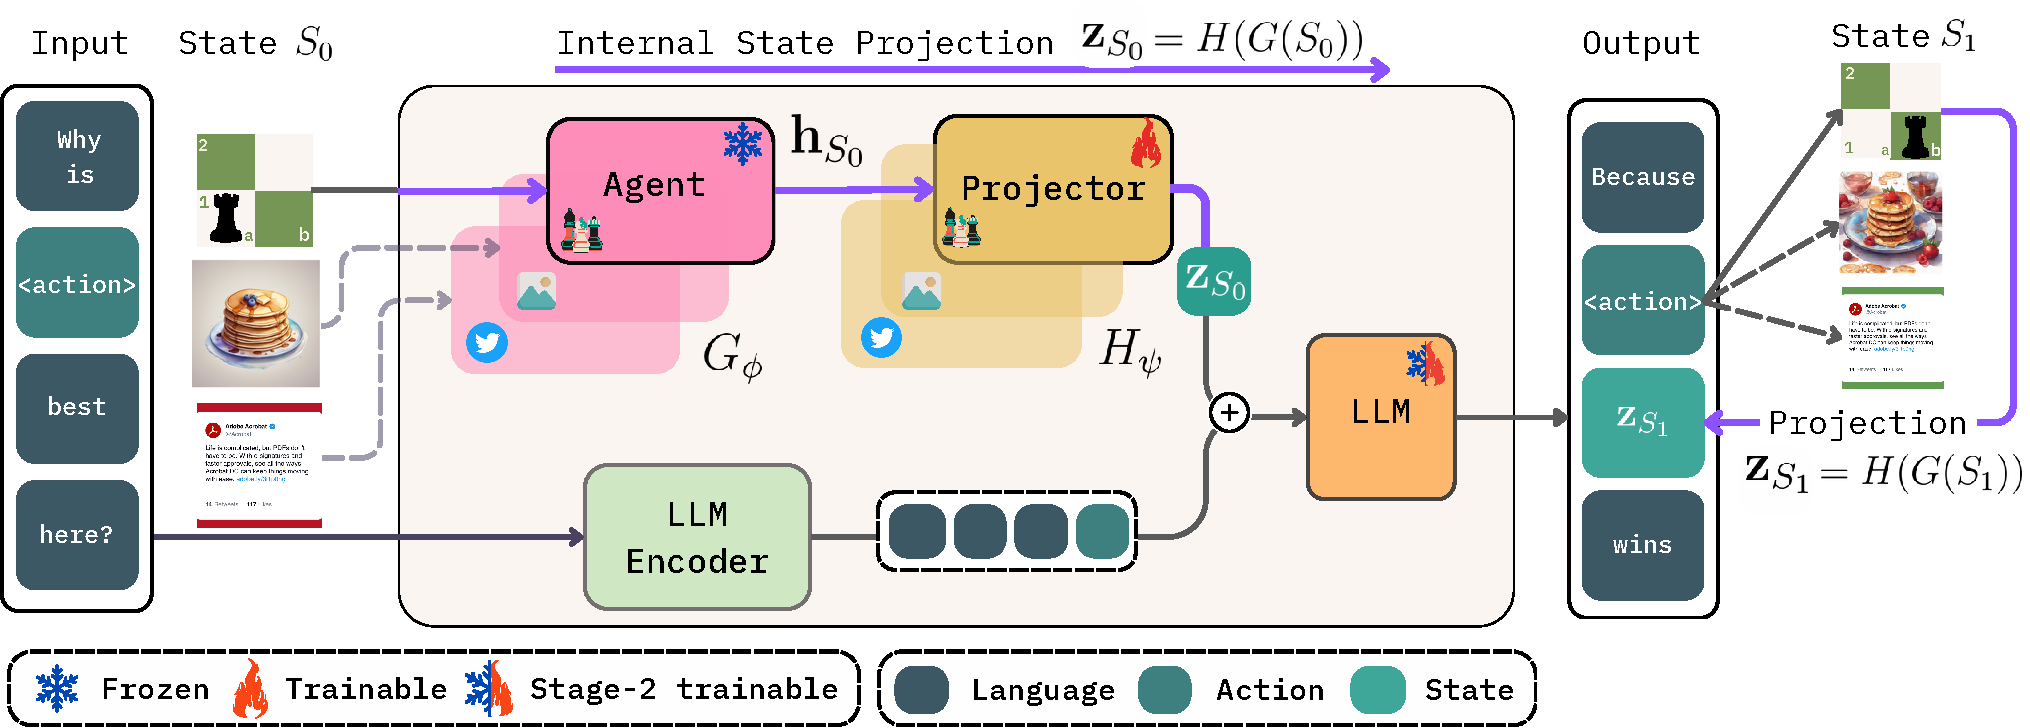
\includegraphics[width=0.98\linewidth]{llamia-fig (5).pdf}
    \caption{\textbf{LLAMIA Architecture Overview.} Given a state $S_0$ (e.g., images, tweets, or board configurations) and a language instruction, the agent's encoder representation $h_{S_0}$ is projected into the LLM's embedding space (indicated by \textcolor[HTML]{8C25FF}{\(\rightarrow\)}) as the internal state projection $z_{S_0}$ and gets concatenated with the LLM language and \texttt{<action>} tokens. During \textit{pretraining}, only the projector $H_\psi$ is trained, while during \textit{fine-tuning}, both the LLM and the projector are jointly trained. At inference time, the LLM uses a special \texttt{<InvokeAgent>} token followed by the state input to explicitly query the agent’s understanding. This allows the model to reason over both the current and counterfactual states.
}
    \vspace{-3mm}
    \label{fig:LLAMIA}

\end{figure}
% \begin{figure*}[t]
%     \centering
%     \begin{subfigure}[b]{0.48\textwidth}
%         \centering
%         \includegraphics[width=\textwidth]{llamia-fig (1).pdf}
%         \caption{LLAMIA architecture}
%         \label{fig:LLAMIA}
%     \end{subfigure}
%     \hfill
%     \begin{subfigure}[b]{0.51\textwidth}
%         \centering
%         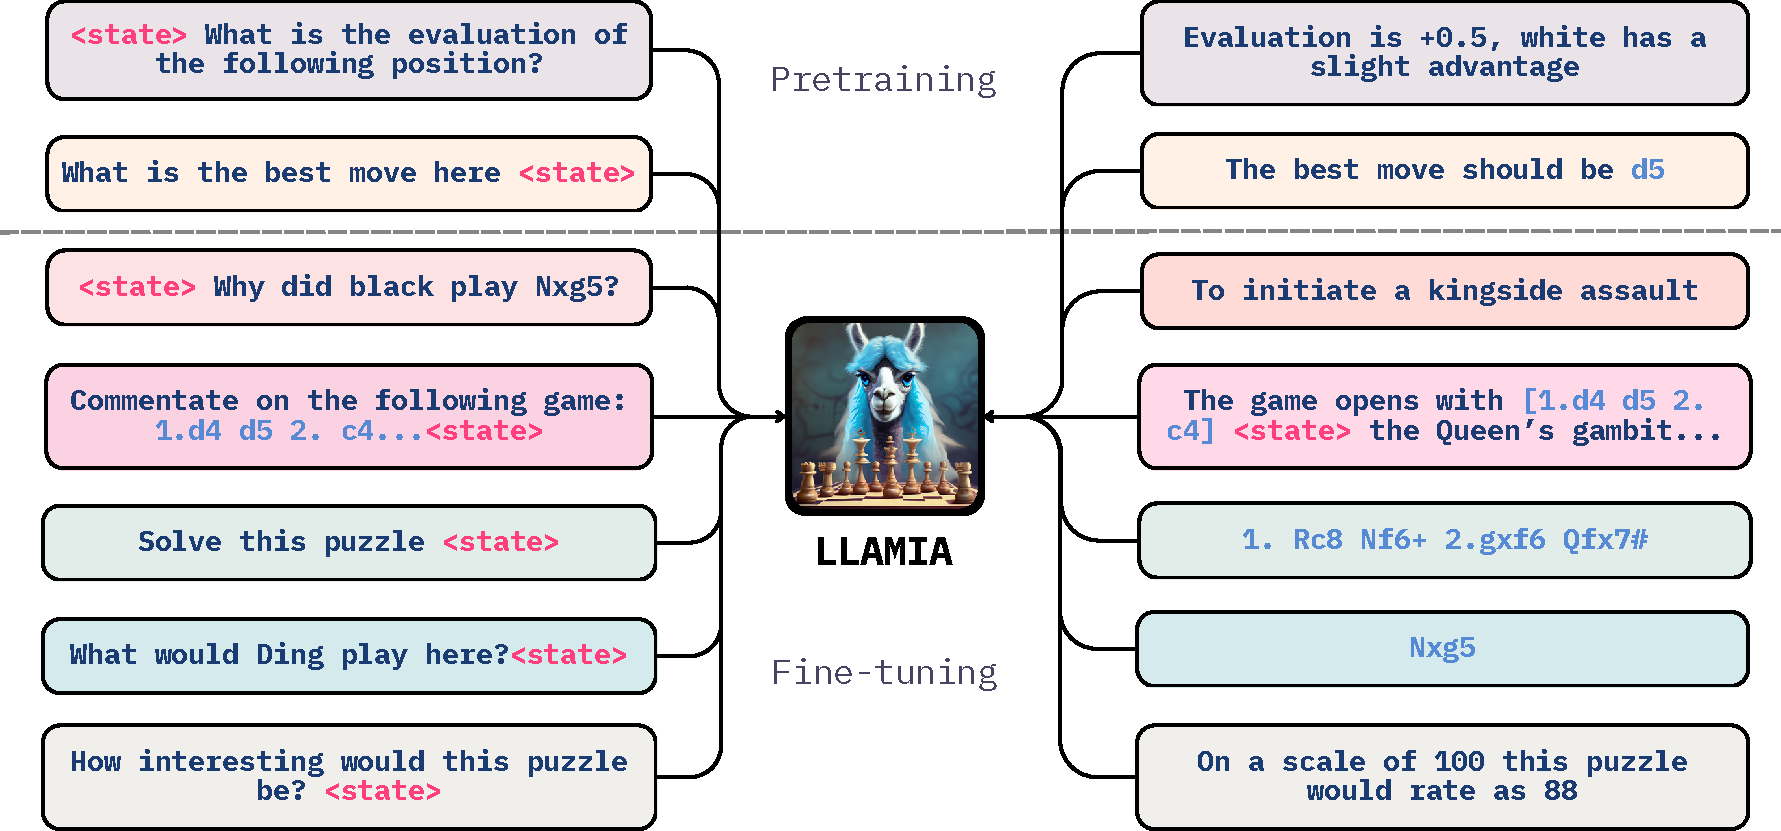
\includegraphics[width=\textwidth]{llamia-tasks3.pdf}
%         \caption{Sample question-answers by LLAMIA demonstrating its capabilities}
%         \label{fig:LLAMIA-alt}
%     \end{subfigure}
%     \vspace{-2mm}
%     \caption{(a) The LLAMIA architecture shows the projection of input states, generation of actions, and language. Actions, encoded in `\textbf{[]}', are extracted by regex  and update the state $S_0$ using the python-chess UCI, and the new state's tokens get appended. Only the projector gets trained for pre-training task, whereas during fine-tuning both LLM and projector get trained. (b) Tasks demonstrating LLAMIA capabilities. The various tasks focus on planning, reasoning, and acting capabilities. The figure shows LLAMIA performing chess evaluations, best move predictions, Behavior Cloning, Commentary Prediction, State Annotation, and Puzzle Understanding, demonstrating the model's ability to simulate human play and analyze game states. \yaman{in b - remove the pertaining, finetuning distinction} }
%     \label{fig:LLAMIA-arch-tasks}
%  \vspace{-3mm}   
% \end{figure*}
% \vspace{-3mm}








% \section{Related Work and Preliminaries}
% Recent research has seen the focus shift to real-life applications that involve topics like long-term reasoning, planning, and search \cite{wei2022emergent,strohman2005indri,huang2022inner,brohan2022rt} which have been core to the field of sequential decision making. Planning and reasoning are important for XXX. Recently, literature has paid much attention to developing these capabilities through various means like using run-time compute in the form of language \cite{XXX} and external tools (e.g., \cite{komeili2021internetaugmenteddialoguegeneration,gao2023pal}), supervised fine-tuning (e.g., \cite{ruoss2024grandmaster,tang2024mathscale,nye2021show,rajani2019explain}). 


%%%%%%%%%%%%%%%%%%%%%%%%%%%%%%%%%%%%%%%%%%%%%%%%%%
%%%%%%%%%%%%%%%%%%%%%%%%%%%%%%%%%%%%%%%%%%%%%%%%%%
%%%%%%%%%%%%%%%%%%%%%%%%%%%%%%%%%%%%%%%%%%%%%%%%%%
%%%%%%%%%%%%%%%%%%%%%%%%%%%%%%%%%%%%%%%%%%%%%%%%%%

\section{Methodology}
\label{sec:methodology}
\vspace{-2mm}
We introduce the LLAMIA framework and its two-stage training approach \textbf{SALT}, designed to internalize latent representations from a pretrained agent directly into the LLM’s autoregressive reasoning process. This integration is achieved by interleaving \textbf{S}tate embeddings, verbalized \textbf{A}ctions, and \textbf{L}anguage \textbf{T}okens in a single sequence, as shown in Figure \ref{fig:LLAMIA}, enabling enhanced planning and reasoning to test our hypothesis in eq\ref{eq:llamia_agent_objective}.

\subsection{Architecture}
\textbf{Pretrained Agent:} 
We employ a pretrained agent $\mathcal{A}$ with policy $\pi(s)$ and encoder backbone \(G_{\psi}: \sS \rightarrow \R^{d}\) where $\psi$ parameterizes the agent's encoder network and $\sS$ is the state space. For any state $s \in \sS$, the agent produces a latent representation: \(\vh_{s} = G_{\psi}(s).\) We use Lc0-BT4, a 15-layer Transformer encoder (240M parameters) optimized for capturing positional features and implicit planning \cite{jenner2024evidence}.

\textbf{Pretrained Large Language Model} We instantiate $F_{\theta}$ with Vicuna~\cite{zheng2023judging} 7B and 13B. To enable the LLM to accept \emph{state} from the agent, we introduce a special token $\langle\text{state}\rangle$. Following an approach similar to LLaVA~\cite{liu2023visual}, we reserve $k$ contiguous token positions to serve as placeholders for any given state $s$. Concretely, whenever $\langle\text{state}\rangle$ is encountered, the model expects $k=16$ (chosen empirically) token embeddings that represent the input state.

\textbf{Agent-to-LLM Projector}
To transform the agent's latent representation $\vh_{s}$ to the LLM's token embedding space, we define a projection network \(H_{\varphi}: \R^{d} \to \R^{k \times e},\) where $\varphi$ parameterizes this projector, $d$ is the dimensionality of the agent's latent representation and $e$ is the hidden dimension (embedding size) of the LLM. Given a latent state embedding $\vh_{s}$, we compute: \(\vz_{s} = H_{\varphi}(\vh_{s})\). The output $\vz_{s}$ has shape $k \times e$ facilitating each of the $k$ special tokens corresponding to $\langle\text{state}\rangle$ in the LLM's. As illustrated in figure \ref{fig:LLAMIA} LLAMIA's input is 
mixed sequences like \([w_1, \langle\text{state}\rangle^{1:k}, a_1, w_2]\), where \(w_i\) is text and \(a_i\) are actions (`Nc2') making it straightforward for the LLM to attend to language, state, and actions together. We implement $H_{\varphi}$ as a three-layer MLP with GeLU activation.

\subsection{SALT: Two-Stage Training Framework}  
To effectively integrate agent representations into the LLM, we propose a two-stage framework (SALT). Stage 1 grounds agent latent states into the LLM's token embedding space. Stage 2 adapts the resulting model to diverse instruction based decision making and reasoning tasks. This ensures that the model can both interpret agent states and perform complex decision-making tasks in a language-aligned manner. The staged training approach addresses data asymmetry, ensures computational efficiency, and maintains training stability.

\subsubsection{Stage 1: Agent Projector Pretraining}

In the first stage, we train only the projection network \(H_\varphi\) to align the agent’s latent representations \(\vh_s\) with the LLM’s token embedding space, while keeping the language model \(F_\theta\) frozen. This alignment allows the LLM to interpret the projected agent state \(\vz_s = H_\varphi(\vh_s)\) as a meaningful planning signal. We construct a large-scale dataset \(\mathcal{D}_{\text{pre}} = \{(s, \pi(s))\}\) by sampling state-policy pairs from the pretrained agent. Each example is paired with a language prompt (e.g., ``Analyze position: top move?''), and the model learns to generate the correct action token corresponding to \(\pi(s)\). The exact prompt is given in Listing \ref{listing:pretraining_instruction_format}. Training minimizes the cross-entropy loss over the correct output conditioned on the projected state and prompt:
\[
\mathcal{L}_{\text{Stage 1}} = -\mathbb{E}_{(s, \pi(s)) \sim \mathcal{D}_{\text{pre}}} \log F_\theta\left( \pi(s) \mid \vz_s, \text{prompt} \right)
\]
This enables fast and stable convergence by leveraging abundant agent-generated data while preserving the pretrained language capabilities of the LLM.

\subsubsection{Stage 2: SALT Fine-Tuning}

The second stage fine-tunes both the LLM \(F_\theta\) and the projector \(H_\varphi\) on a curated dataset \(\mathcal{D}_{\text{SALT}}\) containing interleaved sequences of agent states, verbalized actions, and natural language. This data includes a mixture of state-action demonstrations across skill levels, and natural language explanations of actions. The model learns to handle two types of tasks: generating actions from language instructions and interpreting actions by generating explanatory language conditioned on state embeddings. In both cases, the training objective is the autoregressive cross-entropy loss over the output sequence:
\[
\mathcal{L}_{\text{Stage 2}} = -\mathbb{E}_{(s, \tau, w_{1:T}) \sim \mathcal{D}_{\text{SALT}}} \sum_{t=1}^T \log F_\theta(w_t \mid w_{<t}, \tau, \vz_s)
\]
This stage enables LLAMIA to align decision-making and reasoning with natural language, improving generalization to unseen instructions and planning contexts.

\subsubsection{Internal Search and Agent Invocation}

LLAMIA supports internal look-ahead reasoning by a special token \(\langle\text{InvokeAgent}\rangle\), which triggers a call to the agent policy \(\pi(s')\) on the current or a hypothetical next state \(s'\). The resulting agent embedding \(\vh_{s'}\) is projected to token space via \(H_\varphi\) and inserted into the input sequence as \(\vz_{s'}\), allowing the LLM to accept potential and counterfactual states in inference as context while maintaining autoregressive decoding. 

\paragraph{Efficiency and Stability.}
The two-stage setup improves both efficiency and stability. Stage 1 trains only the lightweight projector on a large dataset of agent outputs, avoiding catastrophic interference with language modeling. Stage 2 fine-tunes the full model on more complex, instruction-rich samples. By decoupling grounding and instruction alignment, SALT enables LLAMIA to learn powerful, language-conditioned policies in a modular and scalable manner.

\begin{comment}
{Stage 1: Agent Projector Pretraining}  
Stage 1 learns a projection from the agent’s latent state $\vh_s$ to a fixed number of LLM token embeddings $\vz_s$, allowing the LLM to interpret state-level planning signals without modifying its own parameters enabling the model to interpret $\vh_s$ as actionable planning signals. Motivated by multimodal alignment in Vision-Language models, here we train the LLM to predict the verbalized top-1 or top-k action (e.g., `Nc2') given a prompt and projected latent state, using standard cross-entropy loss on natural language tokens. Intuitively, we want to reconstruct \( \pi(s) \) directly in language tokens as  \(\text{Verb}\bigl(\pi(s)\bigr)=\text{softmax}(F_{\theta}\bigl(\;\cdot\mid\vz_s,\text{prompt}\bigr))\)
where prompt and Verb$(\pi(s))$ refers to the agent's capabilties (e.g., ``Analyze the position$\rightarrow$Top move Nc2''), the exact format can be seen in listing \ref{listing:pretraining_instruction_format}. 

Since any policy can extract observations and next best action, this method is both, extensible to variety of environments like driving, robotics, and marketing, and we can reliably obtain a large dataset $\mathcal{D}_{pre}$ of state, observations pairs. In this stage the LLM $F_\theta$ is frozen, and only the projector $H_\varphi$ is trained. This ensures that the agent's planning capabilities are effectively mapped into the LLM's token embedding space without destabilizing the pretrained components.

{Stage 2: Instruction-Action Fine-Tuning}
Stage 2 adapts the model to diverse decision making and understanding tasks by fine-tuning both \(F_\theta\) and \(H_\varphi\) on \(\mathcal{D}_{\text{SALT}}\), a dataset interleaved data of states, actions, and language or prompts which can be instructions, questions, or context. \(\mathcal{D}_{\text{SALT}}\) presents two new task paradigms: \textit{language-to-action} and \textit{action-to-language}.  

\textbf{Language-to-Action Tasks} involve generating actions from natural language instructions on a given state. Formally, given an instruction $\tau$ (e.g.``Play like an 1800 rated human'') , a policy $\pi_\tau$ which fulfils $\tau$ and state $s$, we want to achieve:
\vspace{-2mm}
\[
\text{Verb}\bigl(\pi_{\tau}(s)\bigr)=\text{softmax}(F_{\theta}\bigl(\;\cdot\mid\vz_s,\tau\bigr))
\]

\textbf{Action-to-Language Tasks} involve reasoning over actions and states in natural language like explaining the rationale behind a move as seen in figure \ref{fig:LLAMIA} (``Explain the move Nc2''). Formally, given a question $\tau$ we want the LLM to correctly answer $w_{1:T}$(``Since Ra2 leads to mate in 3'') as \[w_{1:T}=\text{softmax}(F_{\theta}\bigl(\;\cdot\mid\vz_s,\tau\bigr))\]

Formally, in both stages, the training objective minimizes the cross-entropy loss for predicting the output $w_{1:T}$ conditioned on the projected state embedding \(\vz_s = H_\varphi(\vh_s)\) and prompt $\tau$ for datasets $\mathcal{D}_{pre}$, $\mathcal{D}_{SALT}$ and parameters $\varphi$, $\{\varphi,\theta\}$ respectively.
\vspace{-2mm}
\begin{equation}
\mathcal{L} = -\mathbb{E}_{(s,\tau,w_{1:T}) \sim \mathcal{D}} \sum_{t=1}^T \log \pi_\theta(w_t \mid w_{1:t-1}, \tau, \vz_s),
\label{eq:llamia_pretrain_objective}    
\end{equation}

\textbf{Efficiency and Stability} The two-stage design ensures parameter-efficient adaptation. In Stage 1, only the projector $H_\varphi$ is trained, representing a small fraction of the total model parameters on a larger dataset. In Stage 2, both the LLM and the projector are fine-tuned on a smaller set of diverse and complex sequences. By decoupling the grounding of agent states from instruction-following fine-tuning, the framework ensures stable and efficient training while enabling the model to perform complex, language-aligned decision-making tasks.

\end{comment}

\begin{table}[h]
    \centering
    \begin{adjustbox}{max width=0.97\textwidth}
    \begin{tabular}{lc|cc|cc|cc|c|cc}
    \toprule[1.2pt]
    \textbf{Model} & \textbf{\#Param} & \multicolumn{2}{c|}{{\small\textbf{Behavior Cloning}}} & \multicolumn{2}{c|}{{\small\textbf{Commentary}}} & \multicolumn{2}{c|}{{\small\textbf{Gameplay}}} & {\small\textbf{Planning}} & \multicolumn{2}{c}{{\small\textbf{Understanding}}} \\ 
    \cmidrule[1pt]{1-11}
     & & {\small\makecell{\textbf{MAIA}\\Acc.}} & {\small\makecell{\textbf{\llamiabench{Bench}}\\Acc.}} & {\small\makecell{\textbf{State}\\BLEU}} & {\small\makecell{\textbf{\llamiabench{Game}}\\G-eval}} & {\small\textbf{Elo}} & {\small\makecell{\textbf{Puzzle}\\Acc.}} & {\small\makecell{\textbf{\llamiabench{Winrate}}\\Avg.}} & {\small\makecell{\textbf{\llamiabench{Diff.}}\\$\rho$}} & {\small\makecell{\textbf{\llamiabench{Interest}}\\$\rho$}} \\
    \midrule
    \multirow{2}{*}{\makecell[l]{\textbf{LLAMIA}\\\small{(SALT)}}} & 7B & 0.52 & \valgood{0.47} & 36.4 & 0.49 & 2171\small{$\pm31$} & 90.1 & 14\% & \valgood{0.61} & \valgood{0.42} \\
     & 13B & \valbest{0.55} & \valbest{0.51} & \valbest{46.3} & \valbest{0.61} & \valgood{2279\small{$\pm41$}} & \valgood{92.9} & \valbest{17\%} & \valbest{0.70} & \valbest{0.50} \\
    \midrule
    \multirow{3}{*}{\makecell[l]{\textbf{ChessGPT}\\\small{(IFT)}}} & 3B & 0.08 & 0.13 & 23.0 & 0.31 & - & 27.9 & 1.3\% & 0.48 & 0.41 \\
     & 7B\textsuperscript{\textdagger} & 0.09 & 0.14 & 28.1 & 0.37 & - & 28.5 & 2.5\% & 0.52 & 0.44 \\
     & 13B\textsuperscript{\textdagger} & 0.11 & 0.16 & 31.3 & 0.42 & - & 29.4 & 4.6\% & 0.55 & 0.47 \\
    \midrule
    \makecell[l]{\textbf{GPT-4o}\\\small{(ICL)}} & - & 0.12 & 0.18 & 32.8 & 0.41 & 1310\small{$\pm92$} & 51.9 & 6.1\% & 0.53 & 0.42 \\
    \midrule
    \makecell[l]{\textbf{GPT-4o}\\\small{(React+Lc0)}} & - & 0.17 & 0.28 & 37.3 & \valgood{0.52} & - & - & 9.2\% & 0.53 & 0.42 \\
    \midrule
    \makecell[l]{\textbf{LLaMA-3}\\\small{(ICL)}} & 405B & 0.13 & 0.20 & 34.5 & 0.41 & - & 21.3 & 6.3\% & 0.50 & 0.39 \\
    \midrule
    \makecell[l]{\textbf{LLaMA-3}\\\small{(React+Lc0)}} & 405B & 0.17 & 0.32 & \valgood{38.2} & 0.44 & - & - & \valgood{10\%} & 0.50 & 0.39 \\
    \midrule
    \makecell[l]{\textbf{SOTA}\\\small{(SFT)}} & $\leq$300M & \valgood{0.53} & 0.40 & 34.5 & - & \valbest{2299\small{$\pm15$}} & \valbest{95.4} & - & 0.46 & 0.35 \\
    \bottomrule[1.2pt]
    \end{tabular}
    \end{adjustbox}
    \vspace{2mm}
    \caption{\textbf{Chess Benchmark Results across Key Capabilities.} 
We compare LLAMIA (trained via our proposed SALT framework) to instruction-finetuned (IFT), in-context learning (ICL), tool-augmented models, and supervised task experts across five chess tasks: behavior cloning (MAIA match), commentary (BLEU, G-eval), gameplay (Elo, puzzle accuracy), instruction-conditioned planning (win rate), and state understanding (difficulty and interest alignment). LLAMIA-13B achieves strong generalization across all tasks without using external search at inference time, outperforming GPT-4o and LLaMA-3 405B + Lc0 in planning and commentary while matching or exceeding task-specific SOTA. Notably, it achieves 2279 Elo and 0.61 G-eval without search, and gains 17\% win rate when adapting to opponent weaknesses.
\vspace{-3mm}
}
    \label{tab:chess_benchmarks}
\end{table}
\section{Experiments}
\label{sec:experiments}
We now present experiments that rigorously evaluate LLAMIA’s capability to internalize latent agent states and act enables its robust intrinsic reasoning and planning capabilities. We test its (1) state-of-the-art performance on gameplay and existing benchmarks without explicit search (2) Generalization on unseen downstream tasks and (3) generalization beyond chess into perceptual and behavioral domains such as text-to-image preference alignment and prediction persuasion.

\subsection{Experimental Setup}
\label{sec:exp_setup}
\begin{figure*}[!h]
    \centering
    \begin{subfigure}[b]{0.52\linewidth}
        \centering
        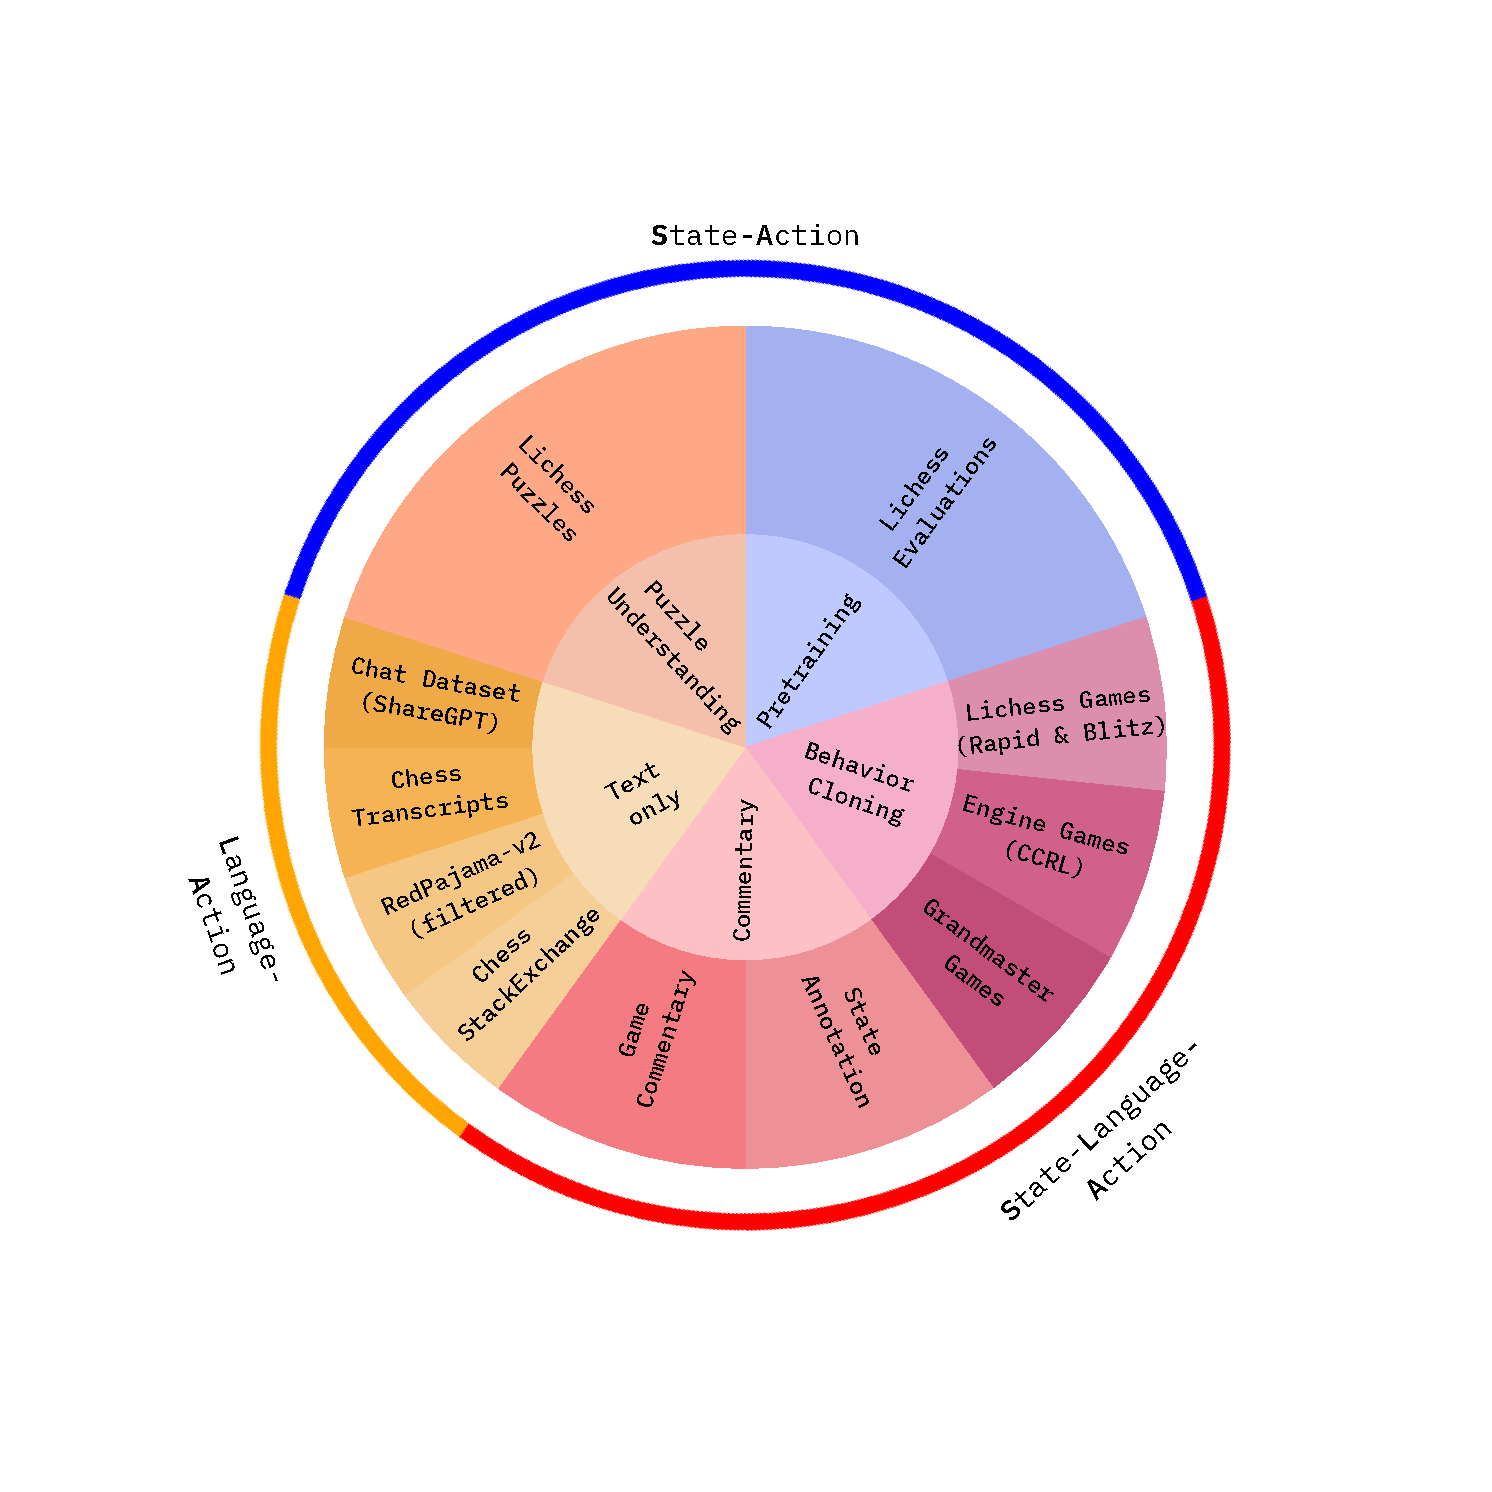
\includegraphics[width=\linewidth]{data.pdf}
        \vspace{-15mm}
        \caption{The inner
circle represents the distribution of training data, detailing the categories. The outer circle lists the types and data sources present in each category.}
        \label{fig:data}
    \end{subfigure}
    \hfill
    \begin{subfigure}[b]{0.45\linewidth}
        \centering
        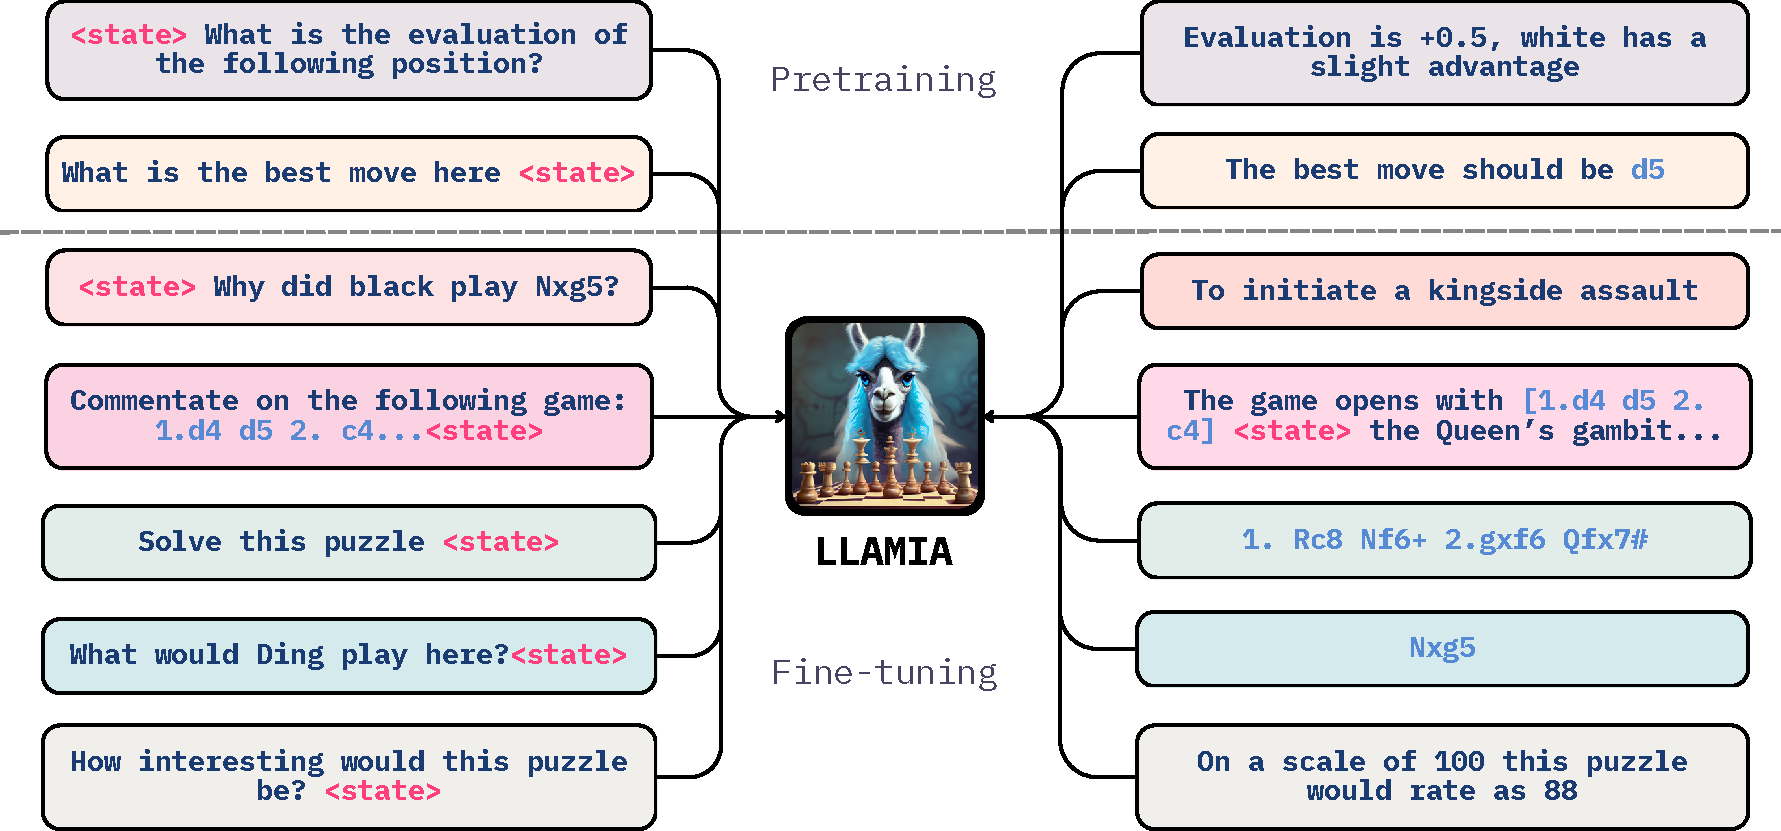
\includegraphics[width=\linewidth]{llamia-tasks3.pdf}
        \caption{Tasks demonstrating LLAMIA capabilities. The various tasks focus on planning, reasoning, and acting capabilities. The figure shows LLAMIA performing chess evaluations, best move predictions, Behavior Cloning, Commentary Prediction, State Annotation, and Puzzle Understanding, demonstrating the model's ability to simulate human play and analyze game states.}
        \label{fig:LLAMIA-arch-tasks}
    \end{subfigure}
 \caption{The above figures detail the data distribution and tasks used to train LLAMIA.}
    \vspace{-2mm}
\end{figure*}

\subsubsection{Datasets} Our evaluations cover a spectrum of decision making scenarios ranging from imitation of human strategies (behavior cloning) and Policy explanation (commentary) to explicit planning conditioned on opponent weaknesses (conditional planning). The datasets for these tasks integrate varying combinations of \emph{states}, \emph{actions}, and \emph{language} contexts (Fig.~\ref{fig:data} and \ref{fig:LLAMIA-arch-tasks}), carefully designed to test LLAMIA’s ability to reason jointly over these modalities. We defer comprehensive dataset statistics, preprocessing details, and precise splits to Appendix~\ref{app:data_stats}.

\subsubsection{Baselines} Given LLAMIA’s claim to efficiently internalize external agent capabilities, we select diverse and rigorous baselines. These include state-of-the-art task-specific experts on each public benchmark, significantly larger general-purpose LLMs (GPT-4o, LLaMA-3 405B) with and without direct agent access through tool-calling (Lc0). We particularly emphasize comparisons that isolate the benefit of our internal latent state projection over standard language model fine tuning (\textit{Proj-Frozen}, ChessGPT) and external agent querying (tool-calling baselines).

LLAMIA models (7B, 13B) were trained on five nodes of 80GB A100 GPUs, totaling approximately eight days of computational budget. Hyperparameters and detailed training schedules are provided in Appendix~\ref{sec:hyperparams}. All reported metrics include bootstrap-derived 95\% confidence intervals to ensure statistically rigorous comparisons.

\subsection{Benchmarks}
\textbf{Grandmaster-level Gameplay without Search}
\label{sec:grandmaster_no_search} To understand whether LLAMIA truly internalizes planning and positional reasoning from latent embeddings alone, we first examine its performance in direct gameplay settings without explicit search. Remarkably, LLAMIA-13B achieves an Elo rating of $2279\pm41$, closely matching the strongest known search-free models and substantially surpassing the state-of-the-art generalist GPT-4o by 969 points (Table~\ref{tab:gameplay-performance}). This outcome supports one of our core hypothesis the internal latent projection alone effectively encapsulates sophisticated positional judgment and implicit planning signals traditionally requiring deep search. Given LLAMIA’s search-free architecture, an intriguing question arises: does latent-state internalization effectively emulate some degree of search? Previous works like \cite{jenner2024evidence} show evidence of learnt lookahead in Lc0-BT4, through mechanistic interpretability. To examine this, we measure Kendall’s $\tau$ correlation between the move probabilities of LLAMIA’s and underlying agent (Lc0-BT4) policy with and without search. Figure~\ref{fig:kt} reveals that, remarkably, LLAMIA’s policy increasingly resembles that of a shallow-search agent as between 30-50M training positions, its alignment with search suddenly increases upto 0.3 and matches a shallow depth of 4.

\begin{figure}[!h]
    \centering
    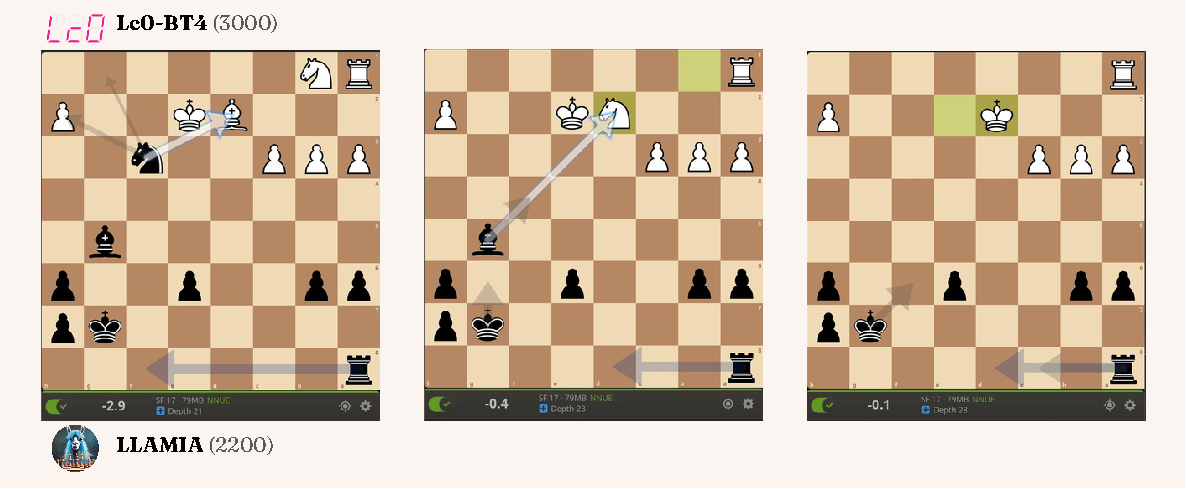
\includegraphics[width=0.95\linewidth]{tcp2.pdf}
    \caption{\textbf{Instruction Conditioned Planning:} LLAMIA is playing against an 800 higher-rated opponent. Note that played moves are indicated with white arrows, and the best moves are shown by blue arrows (size is ordered by the strength of the move). The following instruction is passed: ``your opponent is significantly weaker in endgames''. Orange and yellow moves indicate Mistakes and inaccuracies below. LLAMIA, in this position, plays the move \textbf{\textcolor{orange}{1... Nxd2??}} which is a mistake as it loses its advantage but creates a forced move sequence \textbf{[2. Nxd2 \textcolor{yellow}{Bxd2?} 3. Kxd2]} where it ends with a slightly better position in a rook endgame. Since our task design switches the Elo of Lc0 with a weaker policy here (1500) it ends up winning the game smoothly 19 moves later. LLAMIA was able to plan the forced exchange to trade down in an endgame where it knew it was better, demonstrating its superior planning. \textbf{FEN:[r7/6kp/pp2p2p/6b1/8/PPP2n2/3BK2P/RN6 b - - 0 1]}
}
    \vspace{-3mm}
    \label{fig:tcp}

\end{figure}


\begin{figure}[!h]
    \centering
    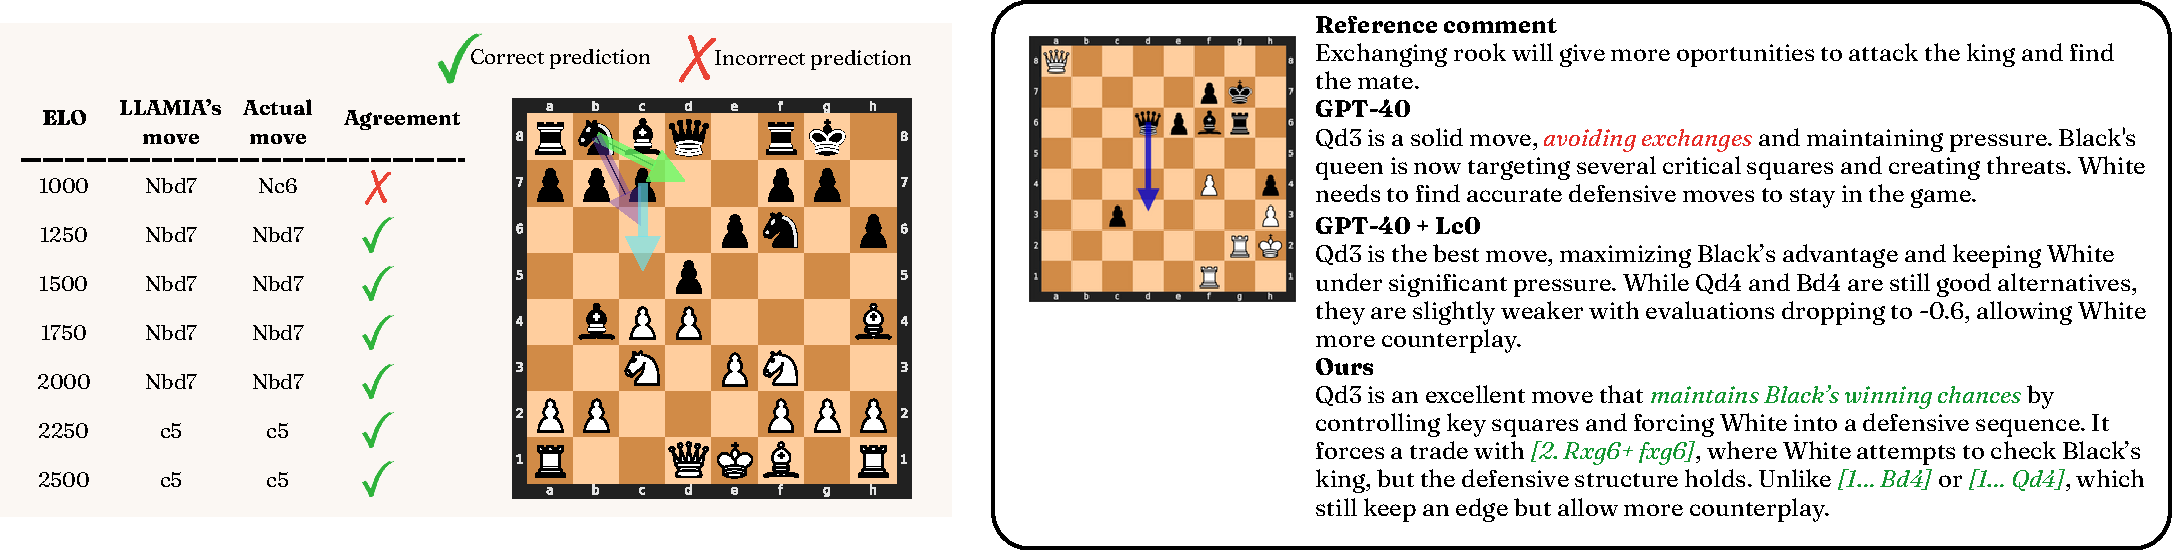
\includegraphics[width=0.98\linewidth]{bc-sc.pdf}
    \caption{\textbf{Left – Behavior Cloning}: The figure presents a qualitative example of behavior cloning. The ``Elo'' column indicates the rating of the players that played the move in this position. ``LLAMIA's Move'' represents the move that LLAMIA would play while simulating a player of that Elo, whereas ``Actual Move'' denotes the move made by a real player at that rating. Notably, LLAMIA successfully predicts the moves across all Elo levels except for 1000, Nearest MAIA (Best of 5) and GPT4o+Lc0 guess 4/7 and 2/7 only. \textbf{Right – State Annotation}:  Examples of generated state annotations. Red text denotes incorrect information, and blue text denotes important concepts and affected counterparts. Green text denotes look-ahead moves. LLAMIA is the only model that explains the position in terms of precise counterfactual states and continuations and shows overall better annotation quality.}
    \label{fig:cloning-annot}
    \vspace{-7mm}
\end{figure}

\textbf{Behavior Cloning} We further probe its capabiliry to clone policies from instructions, which tests a model’s ability to imitate human moves conditioned on player skill levels. Figure~\ref{fig:cloning-annot} shows LLAMIA correctly anticipates moves made by players across a broad Elo spectrum. To further test this we introduce our first LLAMIA-Bench task: Cloning policies in low data regimes like cloning individual grandmasters (GM25), gameplay under time pressure (Time), and when opponent skill has a huge gap $\pm500$. We match or improve over task experts \cite{mcilroy2020aligning} trained on individual skill levels. Detailed ablations of different skill levels and models are given in \ref{tab:behavior_cloning}. We hypothesize that this is a result of jointly training on behaviors and the LLM's ability to distinguish them from text.

\textbf{State Annotation and Game level Commentary}
\label{sec:grounded_commentary}
Generating high quality chess commentary demands contextually relevant move descriptions and identification of subtle strategic themes. Traditional engines offer numerical evaluations but lack expressive explanatory narratives, whereas language only models frequently produce verbose yet superficial annotations. While current research explores move-level commentary \cite{jhamtani-etal-2018-learning}, we extend to game level commentary for commentating an entire game LLAMIA bridges this gap by aligning latent planning signals with fluent commentary generation. Quantitatively, LLAMIA-13B attains a G-eval \cite{liu2023g} score of 0.607, outperforming GPT-4o with tool-calling by 0.086 points while utilizing a model 30 times smaller (Fig.~\ref{fig:commentary}, left). Qualitative inspections (Fig.~\ref{fig:cloning-annot} (right)) further illustrate LLAMIA’s capacity to recognize and articulate nuanced concepts—such as ``passed pawns'' and ``king safety'' which are entirely absent from commentary generated by standard instruction tuned models. 

\textbf{Conditional Planning from Instructions}
\label{sec:instruction_conditioned_planning}

Beyond pure imitation, we explore LLAMIA’s capability to modify its play style according to strategic instructions about an opponent’s known weaknesses. Human chess experts frequently exploit known vulnerabilities such as ``Endgame weakness", ``Time pressure''. Motivated by this human-centric capability, we evaluate LLAMIA using scenarios explicitly constructed to reward such adaptive behaviors (detailed scenario description in Appendix~\ref{tab:instruct_conditioned_planning}). Strikingly, LLAMIA-13B achieves a mean improvement of 17\% over a baseline that cannot condition on instructions (Table~\ref{tab:instruct_conditioned_planning}).
We also observe the generalization capability of LLAMIA by comparing the \% of training data and win rates in \ref{fig:icp}. LLAMIA’s adaptive capabilities emerge rapidly (40\% of training data), whereas standard fine-tuning approaches (ChessGPT-13B) fail to meaningfully adapt until nearly full data exposure. 

\textbf{Generalization to Vision and Persuasion Tasks}
\label{sec:cross_domain}
Finally, we validate LLAMIA’s robustness as a framework beyond chess by integrating latent states from domain-specific pretrained critics in Text-to-Image Preference Alignment and persuasion prediction. For vision-based image preference alignment, LLAMIA significantly surpasses the state-of-the-art VisionReward model (+5 pp accuracy), achieving this improvement with merely half the required fine-tuning data (Appendix~\ref{sec:addl-results}). Qualitative results in Figure~\ref{fig:image_grid} further demonstrate LLAMIA’s superior stylistic fidelity and consistency across diverse artistic prompts.

Similarly, in persuasion modeling—leveraging Chronos-Bolt time-series embeddings—we observe substantial accuracy improvements (+6 pp overall; peaking at +15 pp during weekend spikes; Appendix~\ref{sec:addl-results}). These results concretely demonstrate that LLAMIA’s latent-state integration approach is a broadly applicable mechanism capable of effectively incorporating structured domain knowledge into LLMs, beyond strictly structured game environments.

\section{Limitations and Future Directions}
\label{sec:limitations_future}

Despite compelling results, LLAMIA requires separately trained projectors per domain. Future research could explore meta-learning techniques to enable more scalable multi-domain projector training. Encouragingly, our LoRA fine-tuning ablations (Table~\ref{tab:instruct_conditioned_planning}) indicate that substantial benefits still emerge with minimal parameter updates, highlighting opportunities for deployment-friendly versions of LLAMIA. Additionally, improving LLAMIA’s estimation accuracy in very-low skill scenarios remains an open area for future model refinement.

In summary, LLAMIA robustly demonstrates the power of internalizing latent agent states to achieve expert-level reasoning and strategic flexibility, outperforming much larger externally assisted models and generalizing impressively across perceptual and behavioral domains.





\section{ICML Reviewer comments}

\subsection*{Reviewer ZW8t}

\subsubsection*{Weaknesses}

\begin{itemize}
    \item Clarity of variable definitions in the proposed framework needs to be addressed. In Equation (1), the explanation of variables is confusing. For example, it is unclear what $\mathbf{o}_t$ represents. Are these observations outputs of prior sub-agent calls? Why use the subscript $t$?
    \item The notion of ``prior sub-agent calls'' (lines 112--113) is unclear. What distinguishes $\mathbf{o}_t$ from $\mathbf{s}_t$? What exactly do sub-agent calls return?
    \item The distinction between $\mathbf{s}_t$ and $\mathbf{z}_t$ (lines 119--120) is unclear.
    \item In Figure 2, there is no visible arrow from the agent state to the LLM, despite the text suggesting that the LLM accepts the agent state as input.
    \item Figure and section organization could be improved; figures are sometimes isolated at the ends of pages.
    \item Line 114 defines $\mathbf{a}_t$, but Section 3.2.2 uses both $\mathbf{a}_t$ and $\mathbf{y}_t$ as conditions.
    \item The loss $\mathcal{L}_1$ is described as optimizing the agent projector, but its formulation appears to optimize $\mathbf{y}_t$, creating inconsistency.
    \item Similar ambiguity exists for $\mathcal{L}_2$; the role of the loss function is unclear.
    \item The right panel of Figure 2 is difficult to interpret. It is unclear how $\hat{\mathbf{z}}_t$ is derived, whether it is predicted solely by the LLM, and what the projection from $\mathbf{s}_t$ to $\mathbf{z}_t$ represents conceptually.
    \item Figure 5 refers to blue text annotations that are not present.
    \item Section 4.4 scenarios are difficult to understand without consulting the appendix.
    \item The source of natural language explanations used in Stage 2 training is not described.
    \item Chess-specific metrics such as G-eval and Diff in Table 1 are not explained.
    \item Insufficient details are provided about baselines, including how supervised task experts are trained and how GPT-4o uses agents via tool calling.
    \item No ablation study isolates the effects of Stage 1 versus Stage 2 training.
    \item Section 4.6 mentions LoRA but provides no details or comparisons.
    \item It is unclear what constitutes training versus evaluation data when claiming generalization in Section 4 and Table 1.
    \item Related contemporary work on latent chain-of-thought reasoning is omitted.
    \item Broken hyperlinks and presentation issues reduce readability.
    \item Figure 1 appears too early and contains domain-specific terminology not yet introduced.
    \item Figure 1 contains unlabeled bar plots whose meaning is unclear.
\end{itemize}

\subsubsection*{Questions}

\begin{itemize}
    \item Is there an ablation comparing the use of $\mathbf{s}_t$ versus $\mathbf{z}_t$? What does $\mathbf{z}_t$ contribute beyond using $\mathbf{s}_t$ directly?
    \item What exactly is a ``verbalized action''? Is it generated by the sub-agent, and how does it differ from normal language tokens?
    \item In Figure 1, why does policy-without-search performance drop when pretraining data increases to 30M tokens? What do the bars represent?
    \item In Section 4.3, how often does LLAMIA demonstrate nuanced understanding in practice? Is there any human evaluation or quantitative analysis?
    \item In Figure 5, LLAMIA outputs appear verbose. How should verbosity be interpreted in terms of output quality?
\end{itemize}


\subsection*{Reviewer LEvg}

\subsubsection*{Weaknesses}

\begin{itemize}
    \item The paper lacks formal rigor in its decision-theoretic framing. Claims relating LLM generation to MDPs, POMDPs, and hierarchical RL are made without precise definitions.
    \item Claims of long-horizon planning are not convincingly supported, relying primarily on chess comparisons with GPT-4o.
    \item Comparing a heavily fine-tuned specialized model with general-purpose LLMs using few-shot prompting is not a fair comparison.
    \item Insufficient explanation is provided for the generalization experiments on vision and persuasion tasks, which are relegated to the appendix.
    \item It is unclear how these generalization tasks relate to planning and reasoning, which is the core motivation of the paper.
    \item Presentation issues include unexplained color coding in Table 1 and undefined terms such as ``SOTA (SFT)''.
    \item Figures are poorly placed, with multiple consecutive figures at the end of the paper while key experimental details are deferred to the appendix.
\end{itemize}

\subsection*{Questions}

\begin{itemize}
    \item What do the different color boxes in Table 1 represent?
    \item What methods are referred to by ``SOTA SFT'' in Table 1?
\end{itemize}


\subsection*{Reviewer HUaR}

\subsubsection*{Weaknesses}

\begin{itemize}
    \item The mathematical formalization introduces unnecessary complexity and symbol overloading, leading to inconsistencies in notation and conditioning.
    \item The POMDP framing is misleading since the optimization objectives would require reinforcement learning, which is not used.
    \item The conditioning in the loss formulation appears contradictory, as the model is conditioned on tokens it is also tasked with predicting.
    \item Related work connecting policy networks with LLMs in robotics and autonomous driving is not discussed or differentiated.
    \item Integration with traditional search algorithms is unclear, and the ``Internal Search'' mechanism lacks detail and ablation analysis.
    \item The role of the $\langle \text{InvokeAgent} \rangle$ token is unclear and not demonstrated in examples or datasets.
    \item The experiments focus heavily on chess, limiting claims of general-purpose planning.
    \item Experiments on vision and persuasion tasks lack sufficient methodological detail.
    \item The limitations section is narrow and lacks discussion of broader impacts, particularly given the persuasion experiments.
\end{itemize}

\subsubsection*{Questions}

\begin{itemize}
    \item How does GPT-4o use Lc0 as a tool in practice?
\end{itemize}




Other comments:
1. Planning, reasoning and acting is used too many times and is repetitive, need a better term
2. Other environments: We need to show environments where we can show policy being distilled, instead of framing as a parellel to vision-> language which makes it look like an extension.
3. 

% \begin{figure}[!h]
%     \centering
%     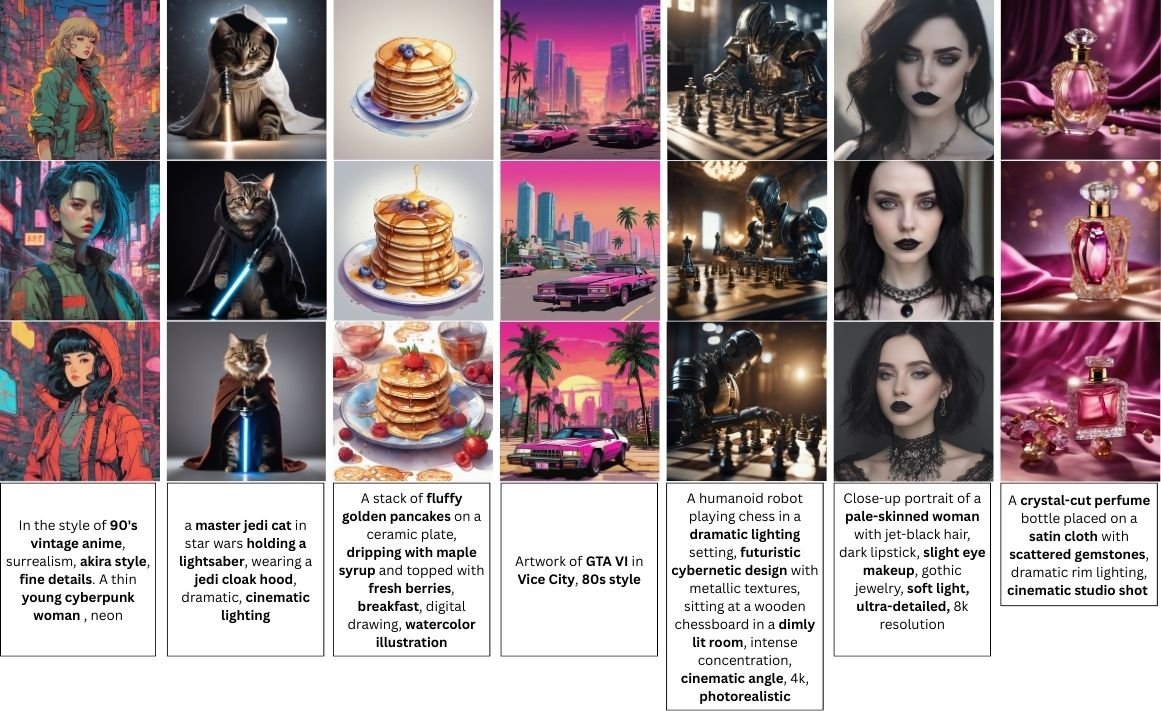
\includegraphics[width=0.7\linewidth]{aesthetics.pdf}
%     \vspace{-1mm}
%     \caption{
% \textbf{Qualitative Examples: Image Preference Alignment via Internalized Rewards.}  
% We compare images generated using VisionReward (left), LLAMIA-ImageReward (middle), and human-preferred selections (right) across diverse prompts involving aesthetic composition, product photography, and stylistic variation. LLAMIA-ImageReward yields more coherent framing, superior lighting consistency, and better adherence to prompt-specific constraints, as also reflected in human preference studies (+5 pp). Notably, these improvements emerge with half the fine-tuning data, demonstrating LLAMIA’s capacity to internalize domain-specific reward functions and generalize stylistic priors across prompts. Full quantitative results appear in Appendix~\ref{sec:addl-results}.
% }.
%     \label{fig:image_grid}
% \end{figure}
% \FloatBarrier

% \textbf{Instruct-Conditioned Planning:} Beyond optimal and human gameplay, we test the ability of these autonomous agents to plan and adapt from instructions in zero-shot. We investigate whether an agent, knowing their opponent is "weaker in endgames," could take suboptimal trajectories that lead to the endgame. When prompted, LLAMIA demonstrates this capability, choosing a notably suboptimal path that forces exchanges to reach the endgame\ref{fig:tcp}. To test Instruction-conditioned planning, we create 5 such scenarios and have LLAMIA play against a much stronger engine from random positions with one caveat: if they reach a position that satisfies the weakness (e.g., Rook Endgame), we swap the engine with a much weaker one. In a tournament of 500 matches, we find that when LLAMIA knows any weakness about its opponent, it wins 17\% more matches. These results are tabulated in table \ref{tab:instruct_conditioned_planning}, with detailed setup explained in section \ref{sec:llamia-bench}. Traditional engines, which cannot take instructions, serve as our baseline and show 0\% improvement, while GPT-4o and LLaMA-405B improve by 3\% and 4\% respectively when assisted with engines. When multiple weaknesses are added, the win rates improve by up to 29\%.

% \textbf{State-Level Commentary:}  Current end-to-end systems for chess game annotation face two significant limitations: they rely on pre-selected moves for annotation rather than autonomously identifying noteworthy positions, and state-of-the-art language models like GPT-4 tend to generate unnecessarily verbose descriptions for well-known positions that traditionally receive concise annotations (e.g., ``this is the Sicilian Opening''). To address these challenges, we propose new metrics for evaluating annotation relevance by (1) measuring models' accuracy in predicting which moves warrant annotation, (2) analyzing length correlation between generated and reference annotations, and (3) computing BLEU-2 scores and perplexity measurements across different annotation categories including descriptive annotations, quality assessments, strategic planning, contextual information, and comparative analysis. This framework enables systematic evaluation of automated chess annotation systems while promoting concise, relevant commentary aligned with traditional chess annotation practices.
%  \ref{tab:state_commentary_annotation}.

% \textbf{Puzzle Understanding} While puzzles have been the testbed for humans and AI over years. We introduce the first work where we benchmark the ability of agents to measure the difficulty and how interesting would humans find them. This benchmark introduces new avenues for understanding decisions. In table \ref{tab:puzzle_understanding} we compare the performance of finetuned Agent embeddings, LLAMIA and GPT-4o.

% Now we outline, popular benchmarks used for evaluating performance in planning and reasoning in chess.
% \begin{figure}[!h]
%     \centering
%     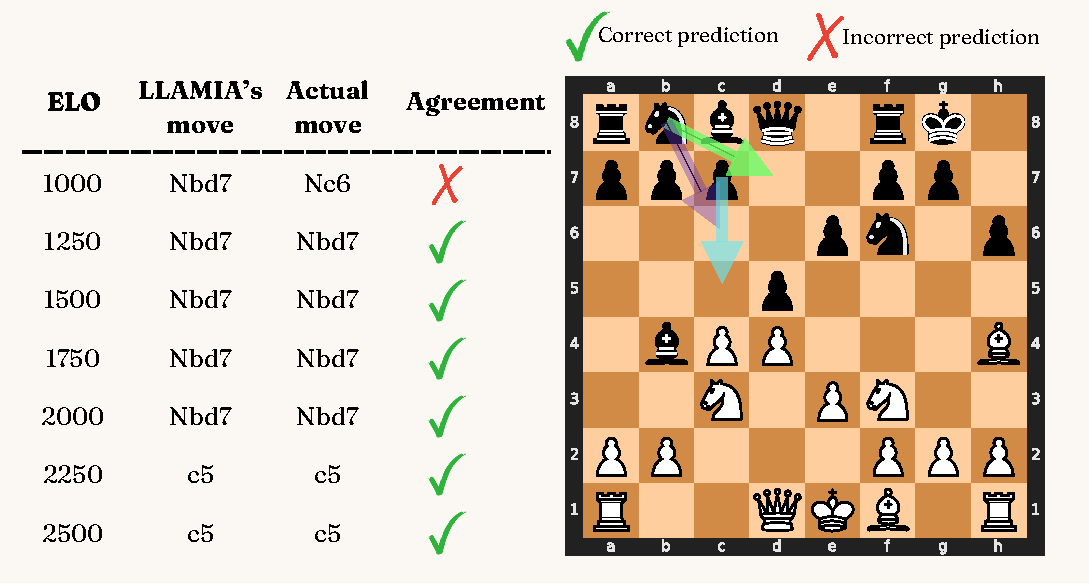
\includegraphics[width=0.4\linewidth]{bc.pdf}
%     \vspace{-1mm}
%     \caption{\textbf{Behavior Cloning}: The figure presents a qualitative example of behavior cloning. The ``Elo'' column indicates the rating of the players that played the move in this position. ``LLAMIA's Move'' represents the move that LLAMIA would play while simulating a player of that Elo, whereas ``Actual Move'' denotes the move made by a real player at that rating. Notably, LLAMIA successfully predicts the moves across all Elo levels except for 1000, Nearest MAIA (Best of 5) and GPT4o+Lc0 guess 4/7 and 2/7 only}
%     \label{fig:cloning-example}
% \vspace{-6mm}
    
% % \end{figure}
% \subsubsection{Behavior Cloning: Move Prediction}
% We evaluate LLAMIA on the MAIA benchmark test set, we find that LLAMIA being a single model is able to clone policies with just text instructions and outperforms previous task experts trained on 10 times more data, in figure \ref{fig:cloning-commentary} we show that depending on the prompt, MAIA is able to predict moves made by actual players from the MAIA test set. We measure move-matching accuracy in table \ref{tab:behavior_cloning} across different Elo brackets, comparing LLAMIA-7B/13B, ChessGPT$^{\dagger}$, MAIA (best-of-5), MAIA+MCTS (best-of-3), and fine-tuned engines (Lc0, Stockfish, AlphaZero). Results demonstrate that LLAMIA-13B achieves state-of-the-art performance in 2-shot settings, surpassing ChessGPT$^{\dagger}$ and improving over MAIA (best-of-5) by 14.6\% and MAIA+MCTS (best-of-3) by 6.9\%.


% \subsubsection{Commentary Generation: Language and Policy}
% Game commentary requires contextualizing moves, identifying strategic themes, and constructing a coherent narrative. Traditional engines evaluate positions numerically, while language models generate fluent but often ungrounded explanations. LLAMIA integrates agent states into its reasoning, enabling move explanations and long-term strategic analysis.  
% Table~\ref{tab:game_commentary_annotation} shows LLAMIA-13B achieves a BLEU-2 score of 57.03, surpassing GPT-4o + Lc0 by over 35 points. It improves commentary relevance to 0.61 correlation, nearly doubling ChessGPT-7B. On planning recall, LLAMIA-13B reaches 0.52, recovering nearly three times more key moves than GPT-4o + Lc0. Evaluation error reduces by 50\% over ChessGPT-7B. These results demonstrate that LLAMIA generates structured, policy-aware narratives without external tool reliance, significantly improving coherence and strategic depth in game analysis.


% \subsection{Searchless Gameplay} We evaluate the ability of the LLAMIA model to mimic the agent. We measure the kendall-tau coefficient and kl-divergence between LLAMIA's and Engine's evaluation (or value) and policy respectively at different depths (refer to figure \ref{fig:kt}). Further to compare the gameplay strength following \cite{ruoss2024grandmaster} in table \ref{tab:gameplay-performance} we calculate the \% of solved puzzles (note that we have a 0\% overlap between test puzzles and training positions) and run an internal tournament between all the agents, we play 50 games per agent pair, and compute the Elo with BayesElo \cite{10.1007/978-3-540-87608-3_11} using the default confidence parameter of 0.5. To ensure variability in the games, we use the openings from Chess Openings (ECO)




% \section{Conclusion}
% In this work, we introduced LLAMIA, a novel framework that seamlessly integrates large language models with internalized agent representations from a pretrained agent to enhance decision-making, planning, and reasoning capabilities. By leveraging a simple yet effective agent projection network, LLAMIA enables LLMs to interact with structured decision tasks in a natural and interpretable manner. Our results demonstrate state-of-the-art performance across a wide range of tasks, including behavior cloning, game-level commentary, puzzle understanding, and instruction-conditioned planning. Notably, LLAMIA outperforms significantly larger models equipped with external tools, underscoring the efficiency of internal agent integration. Beyond chess, the implications of LLAMIA extend to broader decision-making domains such as robotics, autonomous driving, and strategic assistants, highlighting its potential as a foundation for generalized AI reasoning. %Future work could explore extending LLAMIA to real-world tasks requiring multimodal interactions, deeper reasoning, and adaptive planning in dynamic environments. By bridging the gap between language models and structured decision-making, LLAMIA paves the way for more capable, interpretable, and scalable autonomous systems.


% Our approach achieves this through interleaved training on optimal decisions, human strategies, and natural language explanations. These choices are pivotal for training models that generalize across tasks while maintaining robust decision policies and nuanced understanding to bridge reasoning, explanation, and action alignment effectively. Formally, we interleave the \texttt{<state>} tokens, verbalized decision, language, and agent invocations as a conversation for autoregressive training. In the following subsections, we detail the motivation, input-output specifications, and rationale for each training task. Section \ref{XXX} provides comprehensive details on dataset collection, preprocessing, and statistics of the compiled datasets.
    % \subsection{Agent-Projector Pretraining} The primary goal of pretraining is to align the agent's representations with the LLM's latent space. Inspired by approaches in vision, such as LLaVA's use of CLIP for image captioning at scale, we aim to replicate the agent's functionalities through the LLM. Engines evaluate board positions by predicting both a policy and a value, which estimate the next best action and Win/Draw/Loss likelihood. These are in turn used as heuristics for an MCTS-based search to refine into top \textbf{candidate moves}. We train the model to predict these alongside their \textbf{pawn evaluations} (or Q-Values) and \textbf{continuations} (or playouts) given the position's agent projection tokens. Further, we augment this dataset by predicting \textbf{legal moves} and describing salient \textbf{positional features} in natural language, emulating the protocol and state embedding. Listing \ref{listing:pretraining_instruction_format} shows the exact conversation format. This framework mirrors the training paradigm of engines in tabula rasa settings, as the engine self-generates training data, enabling infinite scalability and robust alignment with foundational decision-making tasks. 
% Therefore the LLM is frozen to not only learn the projection matrix from agent to LLM tokens without perturbing the LLM's weights, but scalably learn over a diverse set of positions, for this work we utilize 50M analyzed positions from Lichess.
% \subsection{Pretraining Dataset}
% The purpose of pretraining is to align the agent into the LLM's space. Motivated by similar approaches in vision we aim to mimic the agent's functionalities through the LLM. LLaVA which utilizes clip in its pretraining stage captions the images which are available on a large scale. Similarly the nnue agent returns the value and policy, a UCTS over these results into the evaluation of the positions, and top candidate moves and their continuations or lines. Apart from this the UCI protocol or the environment applies a non linear mask to predict legal moves only. Therefore to project and align the agent's representations and mimic the search into the LLM we train the projector to predict the \textbf{pawn evaluation} of the top candidate moves and their complete \textbf{continuation} given the board \textbf{state}. XXX \% of the time we ask the LLM to predict \textbf{legal moves} and \textbf{describe} the salient features of the position in language to mimic the protocol and state embedding. Akin to an engine's training in tabular rasa settings, all of these are self-generated and scale infinitely.
    
% \subsection{Language Action Finetuning}
% Our Language-Action Fine-tuning dataset is designed to advance the integration of reasoning and decision-making in foundation models.
% % For language-action tasks which require verbal reasoning and planning we create a diverse interleaved Action/Language dataset consisting of the following:



            
% \subsubsection{Behavior Cloning}
% While chess engines have surpassed human performance in chess, the demand for human-like engines remains significant, players prefer competing against bots that emulate human strategies for a more relatable and enjoyable experience, or against "celebrity bots" mimicking renowned grandmasters to engage with iconic playstyles \cite{PlayMagnus,Chess.comBots,LichessbotsXXX}. Grandmasters also use such AI systems to prepare for tournaments by simulating opponents' tactics, enabling them to strategize more effectively. This highlights the importance of behavior cloning in decision-making systems, where the goal is not just optimal performance but the replication of human decision-making processes at varying levels of expertise. Therefore we train LLAMIA to adapt its internal agent's policy to clone behaviours of \begin{enumerate}
%     \item \textbf{Humans}: Predict the evaluation, moves played, and time taken for playing those moves in different positions by Lichess players of different Elos, in different time formats: Listing S5. 

%     \item \textbf{Engines}: Predict moves played by different engines in the CCRL engine tournaments: Listing S4.
%     \item \textbf{Elite}: Predict moves played by prominent grandmasters during tournaments or exhibitions and the winner of the game: Listing S6
% \end{enumerate}

% \subsubsection{Commentary Prediction}
% While chess engines have achieved superhuman levels of play, their ability to provide meaningful commentary or explanations remains underdeveloped. Most engines output variations and numerical evaluations, such as a move being worth +0.39 pawns, which lacks the clarity and context needed for humans to understand and learn. Unlike human grandmasters who can explain the strategic concepts or positional nuances behind their decisions, engines fail to communicate in a way that bridges this 
% knowledge gap. For instance, explaining a -0.39 evaluation as your two isolated pawns outweigh the advantage of a bishop pair and safer king'' transforms a numerical score into actionable insight. Such commentary also democratizes learning, understanding, and enjoying chess, as it explains the complex strategic nuances of the game to viewers, making it more accessible and engaging by breaking down moves, analyzing potential plans, providing historical context, and adding personality to the match. Notably, chess commentators themselves are often rated much lower than prominent grandmasters, yet they skillfully utilize engines to deliver a rich and engaging viewing experience, highlighting the immense potential of explanatory systems to enhance both education and entertainment in chess. High-skilled grandmaster-level commentary or explanations are often limited to major live events or a select few players who have them as personal coaches. Automated systems address this gap by making high-quality insights and strategic explanations broadly accessible.

% We use datasets from prior work in explaining particular positions, commonly known as annotations in chess: Listing S7.

% Further we also introduce game level commentary to explain an entire game: Listing S8

% \subsection{Language Dataset} Recent work \cite{feng2024chessgpt} on bridging engine policies in LLM show great progress through language fine-tuning only, further through training on web scale diverse content previous foundation models like \cite{liu2024improved} have shown improved generalization, so we include diverse language only datasets of chess from the web where curating action finetuning datasets is not trivial. 
% \subsubsection{Chess Stack Exchange} Conversations from chess stack exchange, taken from \cite{feng2024chessgpt}
% \subsubsection{Web} We filtered chess content from the RedPajama-v2 dataset and extend XXX
% \subsubsection{Transcripts} XXX hours of commentary from Chess24 and XXX
% Note that \cite{feng2024chessgpt} uses Webpages and Transcripts for their training but it is not made public, similarly we avoid using their other data sources such as Books, Chessable forums as they might be subject to copyright and therefore make it difficult to compare performance in experimental settings.

% \subsection{Chat Dataset}
% To maintain the multi-turn conversation and general textual reasoning capabilities we augment the fine tuning dataset with XXX ShareGPT conversations which were also used by the base chat model Vicuna \cite{zheng2023judging}

% \subsection{Games}
% We use various data sources to capture game knowledge, including the popular online chess platform Lichess.org, engine games from CCRL( ) and actual games played by grandmasters from the Elite chess database.
% \subsubsection{Lichess}
%  Lichess is a popular, free, open-source chess platform, on which people have played over 1 billion games at a current rate of over 1 million games per day. These games are played live at quick time controls between human players of various skill levels,ranging from total amateurs to the current worldchampion,Magnus Carlsen.  Games are clustered into different formats corresponding to how long they are, including HyperBullet (30 seconds per player), Bullet (1 minute per player), Blitz (3–8 minutes per player), Rapid (8–15 minutes per player), and Classical (longer). In this paper, we ignore games played at the fastest time controls, HyperBullet, since players are often more focused on not losing on time than playing quality moves. We also ignore games over an hr long because very few people actually play longer games with full focus on online platforms. We also filter for games having more than 10 moves and termination being not 'abandoned' which means that the player became inactive or left the game without resigning.

% \subsubsection{CCRL}
% CCRL (Computer Chess Rating Lists) is a data source that provides rating lists for chess engines based on extensive testing. It includes thousands of games played between various chess programs, with results collected into a comprehensive database. Key data points include engine performance under standardized conditions, such as specific time controls (e.g., 40 moves in 15 minutes), endgame tablebases, hash sizes, and use of generic opening books. The ratings reflect the relative strength of chess engines but do not address the originality or legal status of the engines.

% \subsubsection{Elite chess}
% Elite chess data is a collection of games played by grandmasters between the years xxxx-xxxx. There are a total of 158k games spanning famous chess championships like xxx. 

% \subsection{Position Evaluations}

% \subsection{Annotations, StackExchange, Puzzle, Commentary}
% \subsubsection{Annotations}
% The dataset consists of 90k annotated games and chess studies, primarily sourced from Lichess, filtered to include only English annotations. These annotations provide insights into various aspects of the game, including move explanations, game summaries, alternative lines, thematic insights, instructional content, and evaluative comments. They capture strategic ideas, tactical combinations, positional evaluations, and tips, offering rich context for understanding gameplay.

% \subsubsection{StackExchange}
% Chess forum serves as a platform for a large amount of chess-related dialogues and conversations involving a diverse range of users. These platforms encompass high-quality questionand-answer pairs, as seen in platforms like StackExchange, or more generalized discussions on 4various chess-related topics, commonly found in dedicated chess-specific forums. We use 9k StackExchange questions.

% \subsubsection{Puzzle}
% The dataset comprises 4 million chess puzzles sourced from Lichess, a free and open-source chess platform. Each puzzle is derived from actual gameplay and includes metadata such as popularity, opening tags, and ratings.

% Popularity, a measure of community engagement, ranges from -100 (worst) to 100 (best) and is calculated as 
% 100x upvotes - downvotes upvotes + downvotes
% 100× upvotes + downvotes upvotes - downvotes

%  . Votes are further weighted based on factors such as the solver's success rate and their puzzle rating relative to the puzzle's difficulty.

% For puzzles originating in the first 20 moves, we have the OpeningTags which indicates the associated chess opening, chosen from a predefined list. Each attempt to solve a puzzle is treated as a Glicko-2 rated match between the solver and the puzzle, which determines the rating of the puzzle.


% %%%%%

% Puzzles in chess have historically been used to test the understanding of humans as well as engines. Puzzles are specific positions in the game characterized by an objectively winning sequence of moves (typically only one) or \textit{the} solution. Puzzles are further characterized by their themes, difficulty and interestingness. We curate a dataset of 4M puzzles from Lichess and train the LLM to predict the solution, themes, interest, and difficulty of the puzzles. The interestingness of a puzzle is a measure between -100 (worst) to 100 (best) computed using the upvotes and downvotes. Each attempt to solve a puzzle is treated
% as a Glicko-2 rated match between the solver and the puzzle, which determines the rating or the difficulty of the
% puzzle.
    
% Listing S3-XXX










% \section{Experiments}
% \paragraph{Generalised Decision Making}: \textbf{Behavior Cloning}: 
% \cite{dong2024context} XXX
% \cite{guan2024explainable} XXX
% aligning superhuman ai with human behavior- \cite{mcilroy2020aligning}, MAIA2 \cite{tang2024maia}
% , Chess with a bit of search: XXX, MAIA+MCTS \cite{jacob2022modeling}
% Instruction following Decision Making: XXX
% \paragraph{GDU} \textbf{Stylometry} individual behavior in chess- \cite{mcilroy2022learning}, \textbf{Annotation}: \cite{jhamtani-etal-2018-learning}, \cite{zang2019automated} skilled chess engines, \cite{lee2022improving} BART + Chess. 
% \textbf{Reasoning} is the process of thinking about something in a logical and systematic way, using evidence and past experiences to reach a conclusion or make a decision fully supervised fine-tuning - \cite{rajani2019explain, talmor2020leap,nye2021show} it requires a dataset containing explicit reasoning, which can be difficult and time-consuming to create
% \textbf{Puzzle understanding} \cite{10825919}
% \subsection{Behavior Cloning} \ref{tab:behavior_cloning} To evaluate the behavior cloning abilities we test our models on the MAIA Benchmark on cloning moves played by players in a certain Elo range by measuring the move matching accuracy in section XXX we discuss better ways to evaluate this as top-1 accuracy might not be ideal. While cloning players of different playing strength is a great benchmark, a major shortcoming is the lack of generalization in current behavior cloning setups, to mimic the actual gameplay of players many factors such as time-format, opponent, time situation are critical and current methods rely on the abundant number of games available for different Elo subsets. Therefore to further expand the scope of behavior cloning we introduce Behavior Cloning in the wild as an extension in LLAMIA-Bench. Lichess provides an abundant number of games (12M) for these tasks however, in general this amount of data may not be available, therefore we include tasks where the number of observations are quite limited or incomplete including behavior cloning of
% \begin{enumerate}
%     \item GM-25: individual top 25 grandmasters based on peak FIDE rating, the demonstrations are limited because grandmasters can play only a limited number of lifetime games (highest is Victor Korchnoi with 4641 games \cite{XXX}). It is well known \cite{XXX} that these ``super'' grandmasters often play very close to top engine moves, so transforming an optimal policy rather than training from scratch provides an exciting venue here.
%     \item Low-Time: Lichess players when one of the players is under time pressure, this means that the cloning can only be evaluated in an incomplete part of the game. Further players are well known to strategize their gameplay differently when they or their opoonents have lower time \cite{XXX} which is not well approximated by reducing engine depths (check XXX).
%     \item $\Delta Elo$: Lichess players with a huge elo difference, the optimization of cloning approaches so far is done by training or adding search to imitate human gameplay but majority of the gameplay is done of similar rated players and \cite{XXX} it is well known that players differ their gameplay even at the top level when they are matched aganinst an opponent with a skill-gap.

% \end{enumerate}
% \subsection{Behavior Stylometry} ``Guess the Elo'' is a re-occuring question that occurs during interviews, forums, and commentary. Interestingly chess coaches and sometimes even crowdsource are better at identifying the gameplay strengths as opposed to the top grandmaster \cite{XXX}. Understanding individual decision-making styles is a critical step towards foundation decision models that align with human reasoning. In chess, behavioral stylometry focuses on identifying players based solely on their gameplay, revealing unique patterns that define their style. Inspired by methods like \cite{XXX}, we evaluate LLAMIA's ability to distinguish players by their decisions. This allows us to not only identify players but also analyze stylistic nuances that differentiate amateurs from grandmasters or even players of similar expertise. We extend the stylometry task with Grandmaster gameplay classification (GM-25), Human/Engine gameplay classification (Bot), Elo/Strength prediction (Elo), and Time Format prediction as Blitz, Rapid, Classical (Time), thereby broadening the scope from individual-level stylometry to include gameplay classification, skill assessment, and contextual decision-making. We evaluate stylometry using N-way K-shot performance on datasets from Lichess and high-ranked players (High) and GM(25), with all games starting at move 15. Following the exact setup described in \cite{McIlroy-Young2021}, we measure classification accuracy across a pool of candidate players. For Bot, Elo and Time we show multi class classification accuracy on a balanced test set \ref{tab:behavior_stylometry} 
%     \subsection{Commentary}
%         \subsubsection{State Annotation} \ref{tab:state_commentary_annotation} To actually have end to end systems that explain and annotate games, a major current shortcoming is that it is already provided that which move are to be annotated. Further on testing prominent SOTA llms like GPT-4o generate a very verbose description even for well known position which are usually just annotated as ``this is the sicilian opening''. We introduce the metrics to measure the relevance of annotations by making these LLMs predict which moves should be annotated and measuring the length correlation of actual and generated explanations. Further we follow the standard setup of measuring the BLEU-2 and Perplexity of ground-truth and generated annotations for each type of annotation including Description, Quality, Planning, Context, and Comparitive. 

% Description: Explicitly or implicitly describe the current
% move.
% Quality: Describe the
% quality of the current move.
% Comparitive: Compare multiple possible
% moves.
% Planning: Describe the rationale for the current move, in terms of the future gameplay, advantage over other potential moves etc.
% Context: Describe not the current move alone, but the overall game state – such as possibility of win/loss, overall aggression/defence, etc.
        
%         \subsubsection{Game Commentary} In this paper we propose the first game-level commentary or commentating as an expert game commentator as opposed to move annotations. To evaluate on similar metrics as state annotation we introduce the following methods to test game level commentary. Relevance: Length correlation between actual and generated commentaries for move segments for Quality, planning, comparitive and measuring the interest in a certain position, we follow a setup where the generated commentary should be enough for a capable LLM like GPT-4o to predict them.
%         \begin{enumerate}
%             \item Quality: Predict evaluation of the position from the commentary. RMSE of evaluation.
%             \item Planning: Generated and Actual commentary should talk about similar discussed continuation or moves. Recall of moves.
%             \item Comparitive: Predict the correct move from the commentary: Top-1 move accuracy.
%             \item Highlight: Measure the viewer attention at this point in the commentary: RMSE of replay graph obtained from YouTube.
%         \end{enumerate}
%         \ref{tab:game_commentary_annotation}
%         \subsubsection{Chess Coach} Compare with chess.com XXX

% \subsection{Text Condition Planning} While commentary is perceived primarily as explanations of policy combined with artifacts such as game state, known player strategies, wich can be viewed as explanations grounded in policy of super-human agents, environment and players decision history. Here we introduce an interesting and novel task of instruction conditioned policy generation or gameplay with a transformed goal, sub-goals or artifact shortcuts. Traditional planning in chess engines such as AlphaZero or reinforcement learning in general is done assuming optimal gameplay by both players due to which search algorithms like MCTS, Min-max operate for optimal gameplay. But this is not true in real world situations, and grandmasters are known to exploit this, for e.g. Fabiano Caruana a top US GM is known to prepare openings against players with very complex opening positions where an unprepared opponent is likely to lose \cite{XXX}, similarly Magnus Carlsen is known for his feats in endgames \cite{XXX}, Ian Nepomniachi is known for his ability to wriggle out from losing positions with very fast gameplay. Statistically it can be seen with head to head win records of players showing a dissimilar record against different players despite being of very similar average playing strength or Elo. These artifacts exist outside individual gameplay as well, when players are known to be in must-win, or must-not-lose situations they adopt different openings/complicated positions. Therefore to simplify we pose the question as can we use foundational Action models to plan with known strength, weaknesses or opposition information? If an agent knows that its opponent is significantly weaker in endgames will it play slightly suboptimal lines which lead to an endgame? We test this out with our framework described in detail in section XXX and find that XXX.


%         Plan gameplay given player info and weaknesses XXX
%     \subsection{Chess Understanding: ChessGPT Benchmark} XXX
%     With remarks of issues, missing datasets and redundant tables
%         \subsubsection{BigBench State Tracking}
%         \subsubsection{UCI/PGN to FEN}
%         \subsubsection{Chess Annotation Multi-choice} 
%         \subsubsection{Checkmate-in-K}
%         \subsubsection{Opening2PGN and PGN2Opening}

% \somesh{All input, ouput, importance, source}
% \somesh{Tool Calling, ChessGPT 7B}


% \section{Post Training}
% \vspace{6pt}
% \noindent
% \textbf{Predicting Text.}\;
% For \emph{text} tokens $\vz_{i}\in \sV$, we employ a standard language-modeling objective. Specifically, we let $F_{\theta}$ output a distribution over $\sV$:
% \[
%   p_{\theta}(\vz_{i} = w \mid \vz_{1},\ldots,\vz_{i-1}) 
%   = \mathrm{softmax}\bigl(\mathbf{W} \,\vh^{\theta}_{i} + \mathbf{b}\bigr)_{w},
% \]
% where $\vh^{\theta}_{i}$ is the LLM hidden state at position $i$, and $(\mathbf{W},\mathbf{b})$ are the final classification parameters into the vocabulary $\sV$. We then define a cross-entropy loss
% \begin{equation}
% \label{eq:loss_text}
%   \mathcal{L}_{\mathrm{text}} 
%   \;=\; -\, \sum_{\substack{i=1 \\ \vz_{i} \in \sV}}^{n}
%        \log\,p_{\theta}\!\bigl(\vz_{i} \mid \vz_{<i}\bigr).
% \end{equation}

% \noindent
% \textbf{Predicting Actions.}\;
% For tasks with a discrete action space $\langle A_{N}\rangle$ (e.g., next-move predictions in chess), we adopt an \emph{auxiliary decision head} on top of the LLM. Specifically:
% \begin{enumerate}
%     \item We prepend a special token $\langle \text{DECISION}\rangle$ whenever the model is required to output an action.
%     \item Let $\vh^{\theta}_{t}$ be the hidden state corresponding to $\langle \text{DECISION}\rangle$, and let $\vh_{s} = G_{\psi}(\vs)$ be the agent's latent representation of the current state. We concatenate them:
%     \[
%        \vv_{t,s} = [\,\vh^{\theta}_{t}\,\|\,\vh_{s}\,].
%     \]
%     \item A linear layer $I(\cdot)$ maps $\vv_{t,s}$ into $\R^{N}$, producing a distribution over actions:
%     \begin{equation}
%     \label{eq:pred_actions}
%       p\bigl(a = A_{t} \mid \vv_{t,s}\bigr)
%       = \mathrm{softmax}\!\Bigl(I\bigl(\vv_{t,s}\bigr)\Bigr).
%     \end{equation}
% \end{enumerate}
% We train this action head via cross-entropy:
% \begin{equation}
% \label{eq:loss_action}
%   \mathcal{L}_{\mathrm{act}}
%   \;=\; -\, \sum_{A_{t}\in \langle A_{N}\rangle} 
%       \mathbf{1}[\,a=A_{t}\,] 
%       \,\log p\bigl(a \mid \vv_{t,s}\bigr).
% \end{equation}

% % For any task there can be multiple streams of inputs for the state,environment,etc so we consider any agent that learns representations for this, further depending on the task, there can be multiple outputs like Value, Policy etc. Therefore we choose the agent's intermediate fixed size embeddings as the input for our projector. The projector which is a stack of MLPs projects this into the LLM's space as tokens. The LLM takes the actions in text, however for improving environment specific actions (like next move, evaluation) we leverage a single layer auxillary MLP head post training for a small amount of data, this reduces our hallucination rates by XXX\%. These ensure that our architectural choices are extensible. 

% % \subsection{Overall Objective and Inference}
% % Our final training objective combines the text prediction loss \eqref{eq:loss_text} and the action prediction loss \eqref{eq:loss_action}:
% % \begin{equation}
% % \label{eq:combined_loss}
% %   \mathcal{L}
% %   \;=\; \mathcal{L}_{\mathrm{text}} + \lambda\,\mathcal{L}_{\mathrm{act}},
% % \end{equation}
% % where $\lambda$ is a hyperparameter weighting the importance of action classification relative to standard language modeling. In practice, we tune $\lambda$ on a held-out set to balance textual fluency and accurate action decisions.

% % At \emph{inference} time (Fig.~\ref{fig:interleaved}), LLAMIA receives an environment state $\vs$, produces the latent representation $\vh_{s} = G_{\psi}(\vs)$, then projects it into $F_{\theta}$'s token space. The LLM subsequently generates text and, whenever it encounters $\langle \text{DECISION}\rangle$, the auxiliary head $I$ predicts a discrete action from the set $\langle A_{N}\rangle$. Thus, LLAMIA outputs both \emph{language} and \emph{verbal decisions} in a unified autoregressive fashion.

% % \vspace{6pt}
% % \noindent
% % \textbf{Summary.}\;

% %     \item \textbf{Auxiliary Decision Head:} 
% %     For settings with a \emph{fixed-size} action space (denoted $\langle A_{N}\rangle$), such as selecting the next move in chess,\footnote{There are 1858 possible moves in UCI notation for chess.} we incorporate a small classification head to predict environment actions directly. Concretely, after encoding the environment state, we prepend a special decision token $\langle \text{DECISION}\rangle$ to the LLM's output sequence. Let $\vh^{\theta}_{t}$ be the hidden representation corresponding to this decision token within the LLM, and let $\vh_{s}$ be the agent's latent representation of the current state (as above). We form a fused embedding 
% %     \begin{equation}
% %         \vv_{t,s} \;=\; \bigl[\vh^{\theta}_{t} \;\|\; \vh_{s}\bigr],
% %     \end{equation}
% %     where $\|\,$ denotes concatenation. We then feed $\vv_{t,s}$ into a fully connected layer 
% %     \(
% %       I\colon \R^{(\text{dim}(\vh^{\theta}_{t}) + d)} \to \R^{N}
% %     \)
% %     to yield a probability distribution over the $N$ discrete actions:
% %     \begin{equation}
% %         p\bigl(a \mid \vv_{t,s}\bigr) 
% %         \;=\; \mathrm{softmax}\Bigl(I\bigl(\vv_{t,s}\bigr)\Bigr).
% %     \end{equation}
% %     Training uses a standard cross-entropy objective, \emph{i.e.},
% %     \[
% %         \mathcal{L}_{\mathrm{dec}} 
% %         \;=\; -\sum_{a \in \langle A_{N}\rangle} \mathbf{1}_{[\,a = A_{t}\,]}
% %         \,\log\,p\!\bigl(a \mid \vv_{t,s}\bigr),
% %     \]
% %     where $A_{t}$ is the target (ground-truth) action. This decision head allows the model not only to \emph{generate} textual descriptions of actions but also to \emph{predict} them explicitly for downstream environments.
% % \end{enumerate}

% % During inference, given a new environment state $\vs$, we compute $\vh_{s} = G_{\psi}(\vs)$, project it to $\vz_{s} = H_{\varphi}(\vh_{s})$, and then feed $\vz_{s}$ as a series of tokens into $F_{\theta}$. The LLM then generates relevant text and optionally uses the decision token $\langle \text{DECISION}\rangle$ for action prediction, if applicable. Additional fine-tuning or prompt-engineering strategies can be applied for domain adaptation or improved performance.    
% % \item \textbf{Auxillary Decision Head}: For environment-specific fixed-size actions, denoted as $\langle A_N \rangle$, such as selecting the next move in chess \footnote{There are 1858 possible moves in UCI notation.}, we prefix the LLM's output with a special token $t=\mathbf{\langle \text{DECISION} \rangle}$ token. We concatenate the agent's state representation $\mathbf{h}_s$ and the LLM hidden states of the decision token $\mathbf{h}^\theta_t$ to get the action embedding $\mathbf{v}_{t,s}$. We introduce an auxillary decision head, precisely a fully connected layer $I$ to predict the target action $a \sim \langle A_N \rangle$ from the action embedding by maximizing the following objective function with a cross entropy loss. 
% %     \[
% %     P(a=A_t|I(\mathbf{v}_{t,s}))
% %      \]
% %     where $A_t$ is the target action.

% %     \somesh{Post training with inference time projections on a small 50k dataset}


% \section{Results and Discussion}




% % LLaVA training consists of two stages: 
% %(1) feature alignment stage (aka pertaining stage): use our 558K subset of the LAION-CC-SBU dataset to connect a frozen pretrained vision encoder to a frozen LLM; 
% %(2) visual instruction tuning stage: use 150K GPT-generated multimodal instruction-following data, plus around 515K VQA data from academic-oriented tasks, to teach the model to follow multimodal instructions.

% Stage-1 (Pretraining stage): Projector trained on the following tasks:
%     1. Evaluation prediction and top-lines from Lichess eval database (XXX datapoints, Listing XXX)
%     2. State Verbalization prediction (XXX, Listing XXX)
%     3. Move prediction (Engine or Grandmasters or Players) (XXX, Listing XXX)
%     4. Puzzle Solutions (XXX, Listing XXX)

% Stage-2 (action alginment; optional): Projector + LLM DPO on playouts of the form XXX

% Stage-3 (action instruction tuning stage; optional): Projector + LLM Finetuned on the following tasks:
%     1. ChessGPT dataset (Annotations, Games, Stack-exchange) (XXX, Listing XXX)
%     2. Puzzle Themes and Difficulty (XXX, Listing XXX)
%     3. Commentary (2k, Listing XXX)
%     4. XXX (XXX, Listing XXX)



% Comparisons:
%     1. Stage-1 (PT only)
%     2. Stage-1 + Stage-2 (PT + DPO)
%     3. Stage-1 + Stage-3 (PT + AFT)
%     4. Stage-1 + Stage-2 + Stage-3 (PT+DPO+AFT)

%     SL = Supervised Learning
%     RL = Reinforcement Learning


% % \subsection{Policy}
% % \begin{figure}
% %     \centering
% %     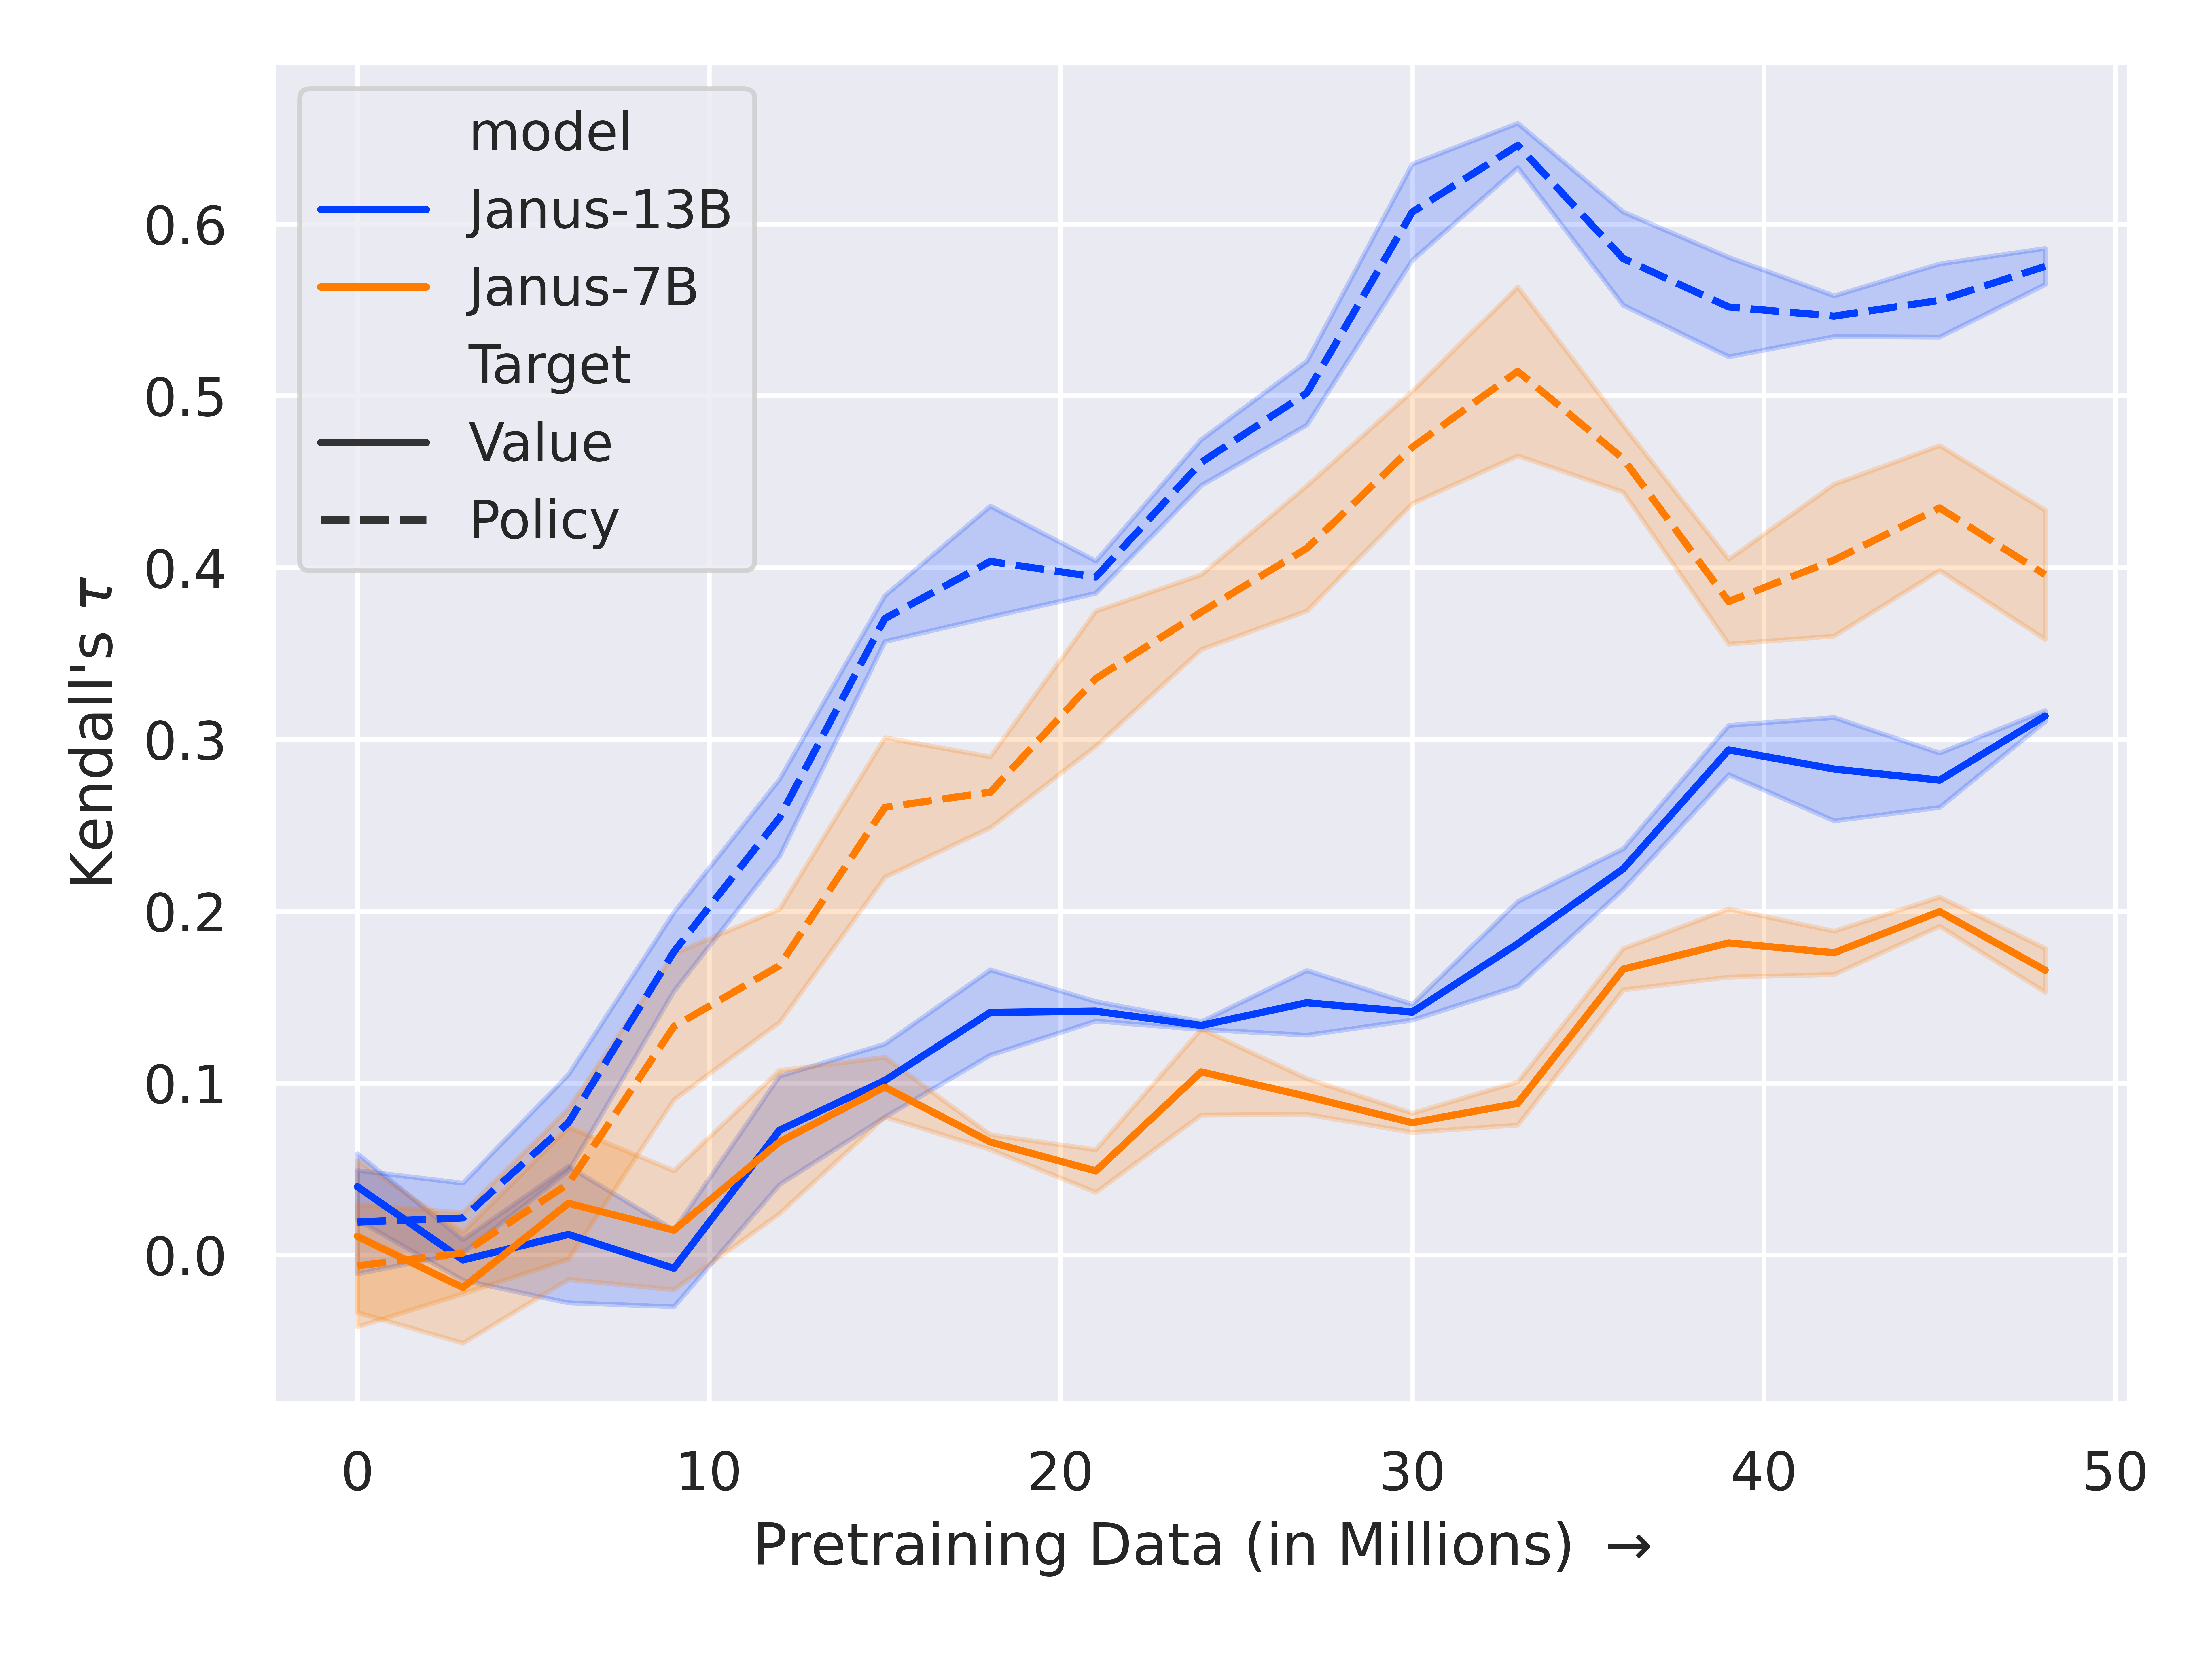
\includegraphics[width=0.8\textwidth]{KendalTau_Alignment.png}
% %     \caption{XXX: Alignment of the model with a search model. Kendall's Tau is calculated between the evals of a search model and FDM. The figure shows that (1)~as the pertaining data increases the (2)~
% %     Reference to say that these are good values since value's Tau is less than 0.45 (XXX)
% %     JK says that it is easier to get policy alignment than a value alignment.
% %     Value - evals 
% %     Policy - Next move 
% %     }
% %     \label{fig:enter-label}
% % \end{figure}






% \begin{figure}
%     \centering
%     \includegraphics[width=0.8\linewidth]{Elo_Gains.png}
%     \caption{
%     Elo vs Epochs - a comparison of three training strategies. 
    
%     CoT-SFT-Oracle/Engine-data - predict the 30 moves (output format - the branch which results in the best move, evals) 
%         Predict 100k Oracle branches 

%     CoT-DPO-Oracle-data - DPO over better branches
%         100k pairs of (oracle better, oracle worse) branches

%     CoT-DPO-generated-data - DPO over better branches
%         100k pairs of (oracle better, FDM worse) branches

%     Prog - SFT in a progressive manner in terms of depth
%         Predict 100k Oracle branches
%     }
%     \label{fig:enter-label}
% \end{figure}


% \subsection{behavior Cloning - Policy Generation}



% \subsection{behavior Cloning - Policy Generation}

% \begin{table}[!h]
%     \centering
%     \begin{adjustbox}{max width=0.5\textwidth}
%     \centering
%     \begin{tabular}{l|c|c|c|c|c}
%     \toprule[1.2pt]
%     \textbf{Model} & \textbf{\#Params} & \textbf{LM Used} & \textbf{Time Series Provided} & \textbf{R\textsuperscript{2}} & \textbf{Simulation} \\
%     \midrule
%     Transsuasion & 13B & Vicuna13B-chat & - & 0.31 & \\
%     Chronos-bolt-base & 205M & T5-untrained & self & 0.09 & \\
%     Chronos-bolt-base & 205M & T5-untrained & self + industry & 0.17 & \\
%     LLAMIA & 13B + 205M & Vicuna13B-chat & self + industry & 0.28 & \\
%     LLAMIA & 13B + 205M & Vicuna13B-chat & self + industry & 0.49 & \\
%     \bottomrule[1.2pt]
%     \end{tabular}
%     \end{adjustbox}
%     \caption{Behavior Simulation}
%     \label{tab:behavior-simulation}
% \end{table}


% \begin{enumerate}
%     \item BigBench State Tracking [Appendix]
%     \item UCI to FEN [Appendix]
%     \item State Value Multi Choice [Appendix]
%     \item Chess Annotation Multi-choice [Why is it broken? How to fix that? Why is behavior Cloning Needed: Past and Future simulation], Multi Choice [Appendix]
%     \item Opening2PGN and PGN2Opening [Appendix]
%     \item Checkmate-in-K [Appendix]
% \end{enumerate}
% \subsubsection{ChessGPT Extension}

% \begin{enumerate}
%     \item Game Masking (Time Format, Player Elo) Analyze GM performance, crowdsource
% \end{enumerate}



% \begin{figure}[!t]
%     \centering
%     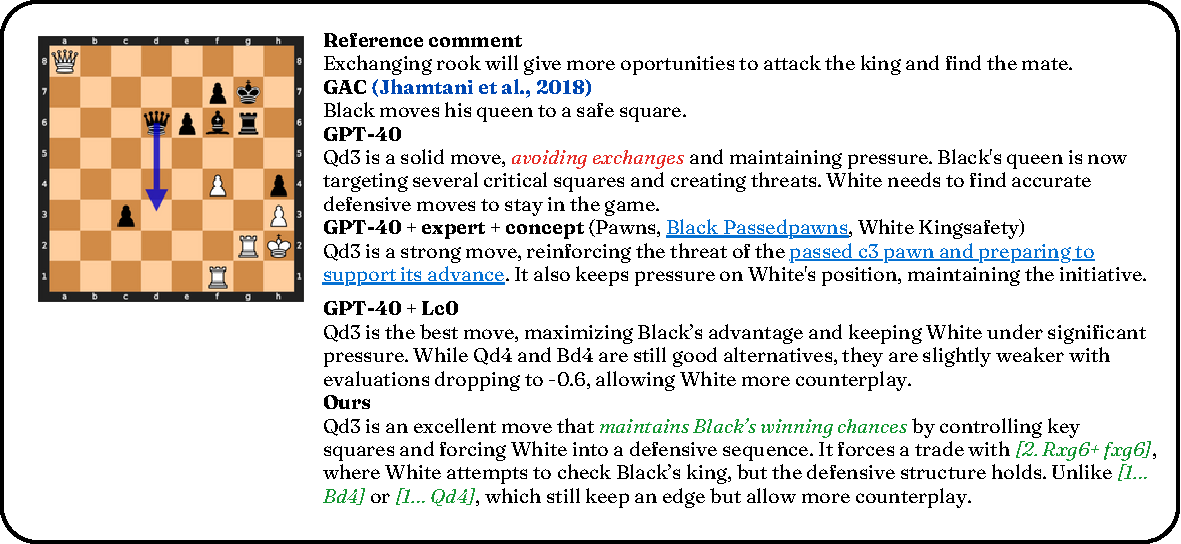
\includegraphics[width=0.45\linewidth]{state-annot4.pdf}
%     \vspace{-5mm}
%     \caption{Examples of generated state annotations. Red text denotes incorrect information, and blue text denotes important concepts and affected counterparts. Green text denotes look-ahead moves. LLAMIA is the only model that explains the position in terms of precise counterfactual states and continuations and shows overall better annotatino quality.}
%     \label{fig:state-annot}
% \end{figure}














% % \section{Introduction}

% % This template is designed to assist with creating a supplemental document to accompany an article in an Optica Publishing Group journal. This template contains example content to help you create your document, and you may use this template as a visual guide. The sections below show examples of different components and styles.


% % \section{Numbering Items in the Supplementary Document}

% % The supplementary materials document may contain additional figures, tables, equations, etc. Such items should be numbered, with an uppercase ``S'' to identify them as supplementary. For example, number the first figure in the supplementary document ``Fig. S1''; the first table ``Table S1''; etc.

% % This template has been designed to automatically format these components with this styling, but we include the naming convention here for reference.

% % \subsection*{Naming Convention for Countable Items}

% % \begin{condenseditemize}
% % \item[] Algorithm S1
% % \item[] Equation (S1)
% % \item[] Figure S1
% % \item[] Media S1
% % \item[] Table S1
% % \end{condenseditemize}


% % \section{Figures and Tables}
% % Figures and Tables should be labeled and referenced in the standard way using the \verb|\label{}| and \verb|\ref{}| commands.

% % \subsection{Sample Figure}

% % Figure \ref{fig:false-color} shows an example figure.

% % \begin{figure}[htbp]
% % \centering
% % \fbox{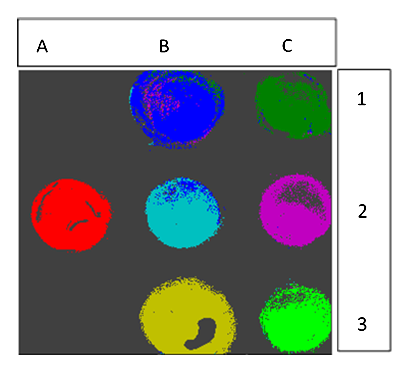
\includegraphics[width=.6\linewidth]{sample}}
% % \caption{False-color image, where each pixel is assigned to one of seven reference spectra.}
% % \label{fig:false-color}
% % \end{figure}

% % \subsection{Sample Table}

% % Table \ref{tab:shape-functions} shows an example table. 

% % \begin{table*}[htbp]
% % \centering
% % \caption{\bf Shape Functions for Quadratic Line Elements}
% % \begin{tabular}{ccc}
% % \hline
% % local node & $\{N\}_m$ & $\{\Phi_i\}_m$ $(i=x,y,z)$ \\
% % \hline
% % $m = 1$ & $L_1(2L_1-1)$ & $\Phi_{i1}$ \\
% % $m = 2$ & $L_2(2L_2-1)$ & $\Phi_{i2}$ \\
% % $m = 3$ & $L_3=4L_1L_2$ & $\Phi_{i3}$ \\
% % \hline
% % \end{tabular}
% %   \label{tab:shape-functions}
% % \end{table*}

% % \section{Sample Equation}

% % Let $X_1, X_2, \ldots, X_n$ be a sequence of independent and identically distributed random variables with $\text{E}[X_i] = \mu$ and $\text{Var}[X_i] = \sigma^2 < \infty$, and let
% % \begin{equation}
% % S_n = \frac{X_1 + X_2 + \cdots + X_n}{n}
% %       = \frac{1}{n}\sum_{i}^{n} X_i
% % \label{eq:refname1}
% % \end{equation}
% % denote their mean. Then as $n$ approaches infinity, the random variables $\sqrt{n}(S_n - \mu)$ converge in distribution to a normal $\mathcal{N}(0, \sigma^2)$.

% % \section{Sample Algorithm}

% % Algorithms can be included using the commands as shown in algorithm \ref{alg:euclid}.

% % \begin{algorithm}
% % \caption{Euclid's algorithm}\label{alg:euclid}
% % \begin{algorithmic}[1]
% % \Procedure{Euclid}{$a,b$}\Comment{The g.c.d. of a and b}
% % \State $r\gets a\bmod b$
% % \While{$r\not=0$}\Comment{We have the answer if r is 0}
% % \State $a\gets b$
% % \State $b\gets r$
% % \State $r\gets a\bmod b$
% % \EndWhile\label{euclidendwhile}
% % \State \textbf{return} $b$\Comment{The gcd is b}
% % \EndProcedure
% % \end{algorithmic}
% % \end{algorithm}

% % \section*{Media}

% % The supplemental document may contain linked objects such as video, 2D, 3D, and machine-readable data files. Please see the \href{https://opg.optica.org/submit/style/supplementary_materials.cfm}{Author Guidelines for Supplementary Materials} for more information. Such files should be cited in the supplementary document as in the primary document but using the naming convention described above.

% % \section*{References} 

% % The supplementary materials document may contain a reference list. The reference list should follow our citation style and should be checked carefully, since staff will not be performing any copyediting. You may add citations manually or use BibTeX. See \cite{Zhang:14}.

% % Citations that are relevant to the primary manuscript and the supplementary document may be included in both places.

% % Bibliography
\clearpage
\bibliography{sample}
\bibliographystyle{icml2025}

% %Manual citation list
% %\begin{thebibliography}{1}
% %\bibitem{Zhang:14}
% %Y.~Zhang, S.~Qiao, L.~Sun, Q.~W. Shi, W.~Huang, %L.~Li, and Z.~Yang,
%  % \enquote{Photoinduced active terahertz metamaterials with nanostructured
%   %vanadium dioxide film deposited by sol-gel method,} Opt. Express \textbf{22},
%   %11070--11078 (2014).
% %\end{thebibliography}
% \appendix

\clearpage
\newpage
\section*{NeurIPS Paper Checklist}

%%% BEGIN INSTRUCTIONS %%%
The checklist is designed to encourage best practices for responsible machine learning research, addressing issues of reproducibility, transparency, research ethics, and societal impact. Do not remove the checklist: {\bf The papers not including the checklist will be desk rejected.} The checklist should follow the references and follow the (optional) supplemental material.  The checklist does NOT count towards the page
limit. 

Please read the checklist guidelines carefully for information on how to answer these questions. For each question in the checklist:
\begin{itemize}
    \item You should answer \answerYes{}, \answerNo{}, or \answerNA{}.
    \item \answerNA{} means either that the question is Not Applicable for that particular paper or the relevant information is Not Available.
    \item Please provide a short (1–2 sentence) justification right after your answer (even for NA). 
   % \item {\bf The papers not including the checklist will be desk rejected.}
\end{itemize}

{\bf The checklist answers are an integral part of your paper submission.} They are visible to the reviewers, area chairs, senior area chairs, and ethics reviewers. You will be asked to also include it (after eventual revisions) with the final version of your paper, and its final version will be published with the paper.

The reviewers of your paper will be asked to use the checklist as one of the factors in their evaluation. While "\answerYes{}" is generally preferable to "\answerNo{}", it is perfectly acceptable to answer "\answerNo{}" provided a proper justification is given (e.g., "error bars are not reported because it would be too computationally expensive" or "we were unable to find the license for the dataset we used"). In general, answering "\answerNo{}" or "\answerNA{}" is not grounds for rejection. While the questions are phrased in a binary way, we acknowledge that the true answer is often more nuanced, so please just use your best judgment and write a justification to elaborate. All supporting evidence can appear either in the main paper or the supplemental material, provided in appendix. If you answer \answerYes{} to a question, in the justification please point to the section(s) where related material for the question can be found.

IMPORTANT, please:
\begin{itemize}
    \item {\bf Delete this instruction block, but keep the section heading ``NeurIPS Paper Checklist"},
    \item  {\bf Keep the checklist subsection headings, questions/answers and guidelines below.}
    \item {\bf Do not modify the questions and only use the provided macros for your answers}.
\end{itemize} 
 

%%% END INSTRUCTIONS %%%


\begin{enumerate}

\item {\bf Claims}
    \item[] Question: Do the main claims made in the abstract and introduction accurately reflect the paper's contributions and scope?
    \item[] Answer: \answerYes{} % Replace by \answerYes{}, \answerNo{}, or \answerNA{}.
    \item[] Justification: The main claims made in the abstract and introduction accurately reflect the
paper’s contributions and scope.
    \item[] Guidelines:
    \begin{itemize}
        \item The answer NA means that the abstract and introduction do not include the claims made in the paper.
        \item The abstract and/or introduction should clearly state the claims made, including the contributions made in the paper and important assumptions and limitations. A No or NA answer to this question will not be perceived well by the reviewers. 
        \item The claims made should match theoretical and experimental results, and reflect how much the results can be expected to generalize to other settings. 
        \item It is fine to include aspirational goals as motivation as long as it is clear that these goals are not attained by the paper. 
    \end{itemize}

\item {\bf Limitations}
    \item[] Question: Does the paper discuss the limitations of the work performed by the authors?
    \item[] Answer: \answerYes{} % Replace by \answerYes{}, \answerNo{}, or \answerNA{}.
    \item[] Justification: We discuss the limitations in the Limitations Section.
    \item[] Guidelines:
    \begin{itemize}
        \item The answer NA means that the paper has no limitation while the answer No means that the paper has limitations, but those are not discussed in the paper. 
        \item The authors are encouraged to create a separate "Limitations" section in their paper.
        \item The paper should point out any strong assumptions and how robust the results are to violations of these assumptions (e.g., independence assumptions, noiseless settings, model well-specification, asymptotic approximations only holding locally). The authors should reflect on how these assumptions might be violated in practice and what the implications would be.
        \item The authors should reflect on the scope of the claims made, e.g., if the approach was only tested on a few datasets or with a few runs. In general, empirical results often depend on implicit assumptions, which should be articulated.
        \item The authors should reflect on the factors that influence the performance of the approach. For example, a facial recognition algorithm may perform poorly when image resolution is low or images are taken in low lighting. Or a speech-to-text system might not be used reliably to provide closed captions for online lectures because it fails to handle technical jargon.
        \item The authors should discuss the computational efficiency of the proposed algorithms and how they scale with dataset size.
        \item If applicable, the authors should discuss possible limitations of their approach to address problems of privacy and fairness.
        \item While the authors might fear that complete honesty about limitations might be used by reviewers as grounds for rejection, a worse outcome might be that reviewers discover limitations that aren't acknowledged in the paper. The authors should use their best judgment and recognize that individual actions in favor of transparency play an important role in developing norms that preserve the integrity of the community. Reviewers will be specifically instructed to not penalize honesty concerning limitations.
    \end{itemize}

\item {\bf Theory assumptions and proofs}
    \item[] Question: For each theoretical result, does the paper provide the full set of assumptions and a complete (and correct) proof?
    \item[] Answer: \answerYes{} % Replace by \answerYes{}, \answerNo{}, or \answerNA{}.
    \item[] Justification: We provide theoretical proofs in the supplementary material.
    \item[] Guidelines:
    \begin{itemize}
        \item The answer NA means that the paper does not include theoretical results. 
        \item All the theorems, formulas, and proofs in the paper should be numbered and cross-referenced.
        \item All assumptions should be clearly stated or referenced in the statement of any theorems.
        \item The proofs can either appear in the main paper or the supplemental material, but if they appear in the supplemental material, the authors are encouraged to provide a short proof sketch to provide intuition. 
        \item Inversely, any informal proof provided in the core of the paper should be complemented by formal proofs provided in appendix or supplemental material.
        \item Theorems and Lemmas that the proof relies upon should be properly referenced. 
    \end{itemize}

    \item {\bf Experimental result reproducibility}
    \item[] Question: Does the paper fully disclose all the information needed to reproduce the main experimental results of the paper to the extent that it affects the main claims and/or conclusions of the paper (regardless of whether the code and data are provided or not)?
    \item[] Answer: \answerYes{} % Replace by \answerYes{}, \answerNo{}, or \answerNA{}.
    \item[] Justification: We have clearly detailed the architecture and training methodology in the Methodology section. We attach the data, benchmark and code as a part of the supplementary material.
    \item[] Guidelines:
    \begin{itemize}
        \item The answer NA means that the paper does not include experiments.
        \item If the paper includes experiments, a No answer to this question will not be perceived well by the reviewers: Making the paper reproducible is important, regardless of whether the code and data are provided or not.
        \item If the contribution is a dataset and/or model, the authors should describe the steps taken to make their results reproducible or verifiable. 
        \item Depending on the contribution, reproducibility can be accomplished in various ways. For example, if the contribution is a novel architecture, describing the architecture fully might suffice, or if the contribution is a specific model and empirical evaluation, it may be necessary to either make it possible for others to replicate the model with the same dataset, or provide access to the model. In general. releasing code and data is often one good way to accomplish this, but reproducibility can also be provided via detailed instructions for how to replicate the results, access to a hosted model (e.g., in the case of a large language model), releasing of a model checkpoint, or other means that are appropriate to the research performed.
        \item While NeurIPS does not require releasing code, the conference does require all submissions to provide some reasonable avenue for reproducibility, which may depend on the nature of the contribution. For example
        \begin{enumerate}
            \item If the contribution is primarily a new algorithm, the paper should make it clear how to reproduce that algorithm.
            \item If the contribution is primarily a new model architecture, the paper should describe the architecture clearly and fully.
            \item If the contribution is a new model (e.g., a large language model), then there should either be a way to access this model for reproducing the results or a way to reproduce the model (e.g., with an open-source dataset or instructions for how to construct the dataset).
            \item We recognize that reproducibility may be tricky in some cases, in which case authors are welcome to describe the particular way they provide for reproducibility. In the case of closed-source models, it may be that access to the model is limited in some way (e.g., to registered users), but it should be possible for other researchers to have some path to reproducing or verifying the results.
        \end{enumerate}
    \end{itemize}


\item {\bf Open access to data and code}
    \item[] Question: Does the paper provide open access to the data and code, with sufficient instructions to faithfully reproduce the main experimental results, as described in supplemental material?
    \item[] Answer: \answerYes{} % Replace by \answerYes{}, \answerNo{}, or \answerNA{}.
    \item[] Justification: We will release the training data, code and benchmark. 
    \item[] Guidelines:
    \begin{itemize}
        \item The answer NA means that paper does not include experiments requiring code.
        \item Please see the NeurIPS code and data submission guidelines (\url{https://nips.cc/public/guides/CodeSubmissionPolicy}) for more details.
        \item While we encourage the release of code and data, we understand that this might not be possible, so “No” is an acceptable answer. Papers cannot be rejected simply for not including code, unless this is central to the contribution (e.g., for a new open-source benchmark).
        \item The instructions should contain the exact command and environment needed to run to reproduce the results. See the NeurIPS code and data submission guidelines (\url{https://nips.cc/public/guides/CodeSubmissionPolicy}) for more details.
        \item The authors should provide instructions on data access and preparation, including how to access the raw data, preprocessed data, intermediate data, and generated data, etc.
        \item The authors should provide scripts to reproduce all experimental results for the new proposed method and baselines. If only a subset of experiments are reproducible, they should state which ones are omitted from the script and why.
        \item At submission time, to preserve anonymity, the authors should release anonymized versions (if applicable).
        \item Providing as much information as possible in supplemental material (appended to the paper) is recommended, but including URLs to data and code is permitted.
    \end{itemize}


\item {\bf Experimental setting/details}
    \item[] Question: Does the paper specify all the training and test details (e.g., data splits, hyperparameters, how they were chosen, type of optimizer, etc.) necessary to understand the results?
    \item[] Answer: \answerYes{} % Replace by \answerYes{}, \answerNo{}, or \answerNA{}.
    \item[] Justification: We have detailed the exact hyperparameters, training and test details in the appendix.
    \item[] Guidelines:
    \begin{itemize}
        \item The answer NA means that the paper does not include experiments.
        \item The experimental setting should be presented in the core of the paper to a level of detail that is necessary to appreciate the results and make sense of them.
        \item The full details can be provided either with the code, in appendix, or as supplemental material.
    \end{itemize}

\item {\bf Experiment statistical significance}
    \item[] Question: Does the paper report error bars suitably and correctly defined or other appropriate information about the statistical significance of the experiments?
    \item[] Answer: \answerYes{} % Replace by \answerYes{}, \answerNo{}, or \answerNA{}.
    \item[] Justification: We have provided error bars in appropriate figures and tables.
    \item[] Guidelines:
    \begin{itemize}
        \item The answer NA means that the paper does not include experiments.
        \item The authors should answer "Yes" if the results are accompanied by error bars, confidence intervals, or statistical significance tests, at least for the experiments that support the main claims of the paper.
        \item The factors of variability that the error bars are capturing should be clearly stated (for example, train/test split, initialization, random drawing of some parameter, or overall run with given experimental conditions).
        \item The method for calculating the error bars should be explained (closed form formula, call to a library function, bootstrap, etc.)
        \item The assumptions made should be given (e.g., Normally distributed errors).
        \item It should be clear whether the error bar is the standard deviation or the standard error of the mean.
        \item It is OK to report 1-sigma error bars, but one should state it. The authors should preferably report a 2-sigma error bar than state that they have a 96\% CI, if the hypothesis of Normality of errors is not verified.
        \item For asymmetric distributions, the authors should be careful not to show in tables or figures symmetric error bars that would yield results that are out of range (e.g. negative error rates).
        \item If error bars are reported in tables or plots, The authors should explain in the text how they were calculated and reference the corresponding figures or tables in the text.
    \end{itemize}

\item {\bf Experiments compute resources}
    \item[] Question: For each experiment, does the paper provide sufficient information on the computer resources (type of compute workers, memory, time of execution) needed to reproduce the experiments?
    \item[] Answer: \answerYes{} % Replace by \answerYes{}, \answerNo{}, or \answerNA{}.
    \item[] LLAMIA models (7B, 13B) were trained on five nodes of 80GB A100 GPUs, totaling approximately eight days of computational budget. More details on training and compute can be found in the appendix.
    \item[] Guidelines:
    \begin{itemize}
        \item The answer NA means that the paper does not include experiments.
        \item The paper should indicate the type of compute workers CPU or GPU, internal cluster, or cloud provider, including relevant memory and storage.
        \item The paper should provide the amount of compute required for each of the individual experimental runs as well as estimate the total compute. 
        \item The paper should disclose whether the full research project required more compute than the experiments reported in the paper (e.g., preliminary or failed experiments that didn't make it into the paper). 
    \end{itemize}
    
\item {\bf Code of ethics}
    \item[] Question: Does the research conducted in the paper conform, in every respect, with the NeurIPS Code of Ethics \url{https://neurips.cc/public/EthicsGuidelines}?
    \item[] Answer: \answerYes{} % Replace by \answerYes{}, \answerNo{}, or \answerNA{}.
    \item[] Justification: Yes, we conform with the NeurIPS Code of Ethics.
    \item[] Guidelines:
    \begin{itemize}
        \item The answer NA means that the authors have not reviewed the NeurIPS Code of Ethics.
        \item If the authors answer No, they should explain the special circumstances that require a deviation from the Code of Ethics.
        \item The authors should make sure to preserve anonymity (e.g., if there is a special consideration due to laws or regulations in their jurisdiction).
    \end{itemize}


\item {\bf Broader impacts}
    \item[] Question: Does the paper discuss both potential positive societal impacts and negative societal impacts of the work performed?
    \item[] Answer: \answerNA{} % Replace by \answerYes{}, \answerNo{}, or \answerNA{}.
    \item[] Justification: This work has no direct societal impact because it describe on architectural improvements and internal agents. The proposed method can be used to equip LLMs with specialized reasoning abilities.
    \item[] Guidelines:
    \begin{itemize}
        \item The answer NA means that there is no societal impact of the work performed.
        \item If the authors answer NA or No, they should explain why their work has no societal impact or why the paper does not address societal impact.
        \item Examples of negative societal impacts include potential malicious or unintended uses (e.g., disinformation, generating fake profiles, surveillance), fairness considerations (e.g., deployment of technologies that could make decisions that unfairly impact specific groups), privacy considerations, and security considerations.
        \item The conference expects that many papers will be foundational research and not tied to particular applications, let alone deployments. However, if there is a direct path to any negative applications, the authors should point it out. For example, it is legitimate to point out that an improvement in the quality of generative models could be used to generate deepfakes for disinformation. On the other hand, it is not needed to point out that a generic algorithm for optimizing neural networks could enable people to train models that generate Deepfakes faster.
        \item The authors should consider possible harms that could arise when the technology is being used as intended and functioning correctly, harms that could arise when the technology is being used as intended but gives incorrect results, and harms following from (intentional or unintentional) misuse of the technology.
        \item If there are negative societal impacts, the authors could also discuss possible mitigation strategies (e.g., gated release of models, providing defenses in addition to attacks, mechanisms for monitoring misuse, mechanisms to monitor how a system learns from feedback over time, improving the efficiency and accessibility of ML).
    \end{itemize}
    
\item {\bf Safeguards}
    \item[] Question: Does the paper describe safeguards that have been put in place for responsible release of data or models that have a high risk for misuse (e.g., pretrained language models, image generators, or scraped datasets)?
    \item[] Answer: \answerNA{} % Replace by \answerYes{}, \answerNo{}, or \answerNA{}.
    \item[] Justification: We do not release any pretrained language model or image generator or any
other model. All data that is used in this paper is curated from publicly available sources.
    \item[] Guidelines:
    \begin{itemize}
        \item The answer NA means that the paper poses no such risks.
        \item Released models that have a high risk for misuse or dual-use should be released with necessary safeguards to allow for controlled use of the model, for example by requiring that users adhere to usage guidelines or restrictions to access the model or implementing safety filters. 
        \item Datasets that have been scraped from the Internet could pose safety risks. The authors should describe how they avoided releasing unsafe images.
        \item We recognize that providing effective safeguards is challenging, and many papers do not require this, but we encourage authors to take this into account and make a best faith effort.
    \end{itemize}

\item {\bf Licenses for existing assets}
    \item[] Question: Are the creators or original owners of assets (e.g., code, data, models), used in the paper, properly credited and are the license and terms of use explicitly mentioned and properly respected?
    \item[] Answer: \answerYes{} % Replace by \answerYes{}, \answerNo{}, or \answerNA{}.
    \item[] Justification: We cite and abide by the license of each of the assets
    \item[] Guidelines:
    \begin{itemize}
        \item The answer NA means that the paper does not use existing assets.
        \item The authors should cite the original paper that produced the code package or dataset.
        \item The authors should state which version of the asset is used and, if possible, include a URL.
        \item The name of the license (e.g., CC-BY 4.0) should be included for each asset.
        \item For scraped data from a particular source (e.g., website), the copyright and terms of service of that source should be provided.
        \item If assets are released, the license, copyright information, and terms of use in the package should be provided. For popular datasets, \url{paperswithcode.com/datasets} has curated licenses for some datasets. Their licensing guide can help determine the license of a dataset.
        \item For existing datasets that are re-packaged, both the original license and the license of the derived asset (if it has changed) should be provided.
        \item If this information is not available online, the authors are encouraged to reach out to the asset's creators.
    \end{itemize}

\item {\bf New assets}
    \item[] Question: Are new assets introduced in the paper well documented and is the documentation provided alongside the assets?
    \item[] Answer: \answerYes{} % Replace by \answerYes{}, \answerNo{}, or \answerNA{}.
    \item[] Justification: We release the data, code and benchmark.The new assets will be well documented when being released.
    \item[] Guidelines:
    \begin{itemize}
        \item The answer NA means that the paper does not release new assets.
        \item Researchers should communicate the details of the dataset/code/model as part of their submissions via structured templates. This includes details about training, license, limitations, etc. 
        \item The paper should discuss whether and how consent was obtained from people whose asset is used.
        \item At submission time, remember to anonymize your assets (if applicable). You can either create an anonymized URL or include an anonymized zip file.
    \end{itemize}

\item {\bf Crowdsourcing and research with human subjects}
    \item[] Question: For crowdsourcing experiments and research with human subjects, does the paper include the full text of instructions given to participants and screenshots, if applicable, as well as details about compensation (if any)? 
    \item[] Answer: \answerNA{} % Replace by \answerYes{}, \answerNo{}, or \answerNA{}.
    \item[] Justification: We don’t involve human subjects
    \item[] Guidelines:
    \begin{itemize}
        \item The answer NA means that the paper does not involve crowdsourcing nor research with human subjects.
        \item Including this information in the supplemental material is fine, but if the main contribution of the paper involves human subjects, then as much detail as possible should be included in the main paper. 
        \item According to the NeurIPS Code of Ethics, workers involved in data collection, curation, or other labor should be paid at least the minimum wage in the country of the data collector. 
    \end{itemize}

\item {\bf Institutional review board (IRB) approvals or equivalent for research with human subjects}
    \item[] Question: Does the paper describe potential risks incurred by study participants, whether such risks were disclosed to the subjects, and whether Institutional Review Board (IRB) approvals (or an equivalent approval/review based on the requirements of your country or institution) were obtained?
    \item[] Answer: \answerNA{} % Replace by \answerYes{}, \answerNo{}, or \answerNA{}.
    \item[] Justification: We don’t involve human subjects.
    \item[] Guidelines:
    \begin{itemize}
        \item The answer NA means that the paper does not involve crowdsourcing nor research with human subjects.
        \item Depending on the country in which research is conducted, IRB approval (or equivalent) may be required for any human subjects research. If you obtained IRB approval, you should clearly state this in the paper. 
        \item We recognize that the procedures for this may vary significantly between institutions and locations, and we expect authors to adhere to the NeurIPS Code of Ethics and the guidelines for their institution. 
        \item For initial submissions, do not include any information that would break anonymity (if applicable), such as the institution conducting the review.
    \end{itemize}

\item {\bf Declaration of LLM usage}
    \item[] Question: Does the paper describe the usage of LLMs if it is an important, original, or non-standard component of the core methods in this research? Note that if the LLM is used only for writing, editing, or formatting purposes and does not impact the core methodology, scientific rigorousness, or originality of the research, declaration is not required.
    %this research? 
    \item[] Answer: \answerYes{} % Replace by \answerYes{}, \answerNo{}, or \answerNA{}.
    \item[] Justification: We use LLMs in our architecture
    \item[] Guidelines:
    \begin{itemize}
        \item The answer NA means that the core method development in this research does not involve LLMs as any important, original, or non-standard components.
        \item Please refer to our LLM policy (\url{https://neurips.cc/Conferences/2025/LLM}) for what should or should not be described.
    \end{itemize}

\end{enumerate}
\clearpage
\appendix

\section*{Appendix}
\section{Dataset}
\label{app:data_stats}
\vspace{-2mm}
In this section, we describe the datasets and on which we train LLAMIA. Extensive research from Flan, LLaVA, QLora \cite{longpre2023flan,dettmers2024qlora,liu2024improved,liu2023visual} demonstrate that joint training across diverse tasks, modalities, and instructions enhances model generalization and zero-shot reasoning. Motivated by this, we train LLAMIA on interleaved datasets that combine agent states, actions, and language instructions. Our approach integrates three objectives: (1) aligning pretrained agents with LLM representations, (2) cloning diverse decision making behaviors, and (3) predicting human explanations. Below we outline the datasets used.

\subsection{Agent-Projector Pretraining}
The pretraining phase aligns the agent’s latent state representations with the LLM’s embedding space. We extract the \textbf{top moves} and their \textbf{pawn evaluations} from the lichess evaluation database \footnote{\url{https://database.lichess.org/\#evals}}. We filter out weaker evaluations to obtain 50 million evaluations. Further, we augment these with positional features such as legal moves, tactical motifs (e.g., pins, forks), and strategic annotations (e.g., king safety, pawn structure) extracted from Chevy\footnote{\url{https://github.com/int8/chevy}}. Listing \ref{listing:pretraining_instruction_format} shows the exact conversation format.

\subsection{Language-Action Fine-Tuning}
\label{subsec:language_action }
\subsubsection{Behavior Cloning}
Behavior cloning is the process of learning policies by mimicking demonstrations. In chess it is used to replicate human-like playstyles, engine strategies, and grandmaster tactics making gameplay more relatable, instructive, and diverse. This dataset is crucial for training LLAMIA to adapt its internal agent’s policy across varying expertise level.

We curate chess games from diverse sources, spanning human and engine play across skill levels. The Lichess dataset includes 12 million rapid and blitz games with Elo ratings between 1000 and 2500. For superhuman play, we incorporate 3 million CCRL games sourced from \cite{feng2024chessgpt},  played by engines like Stockfish and Leela Zero, which have Elo ratings between 2800 and 3700. Additionally, we include 158,000 elite grandmaster tournament games \cite{gmchessgames2022}, providing insights into expert human strategy. Where available, metadata such as player Elo, time control, and annotations are included. Listing \ref{listing:lichess_instruction_format} shows the exact conversation formats. 
During testing, we evaluate behavior cloning on the MAIA-KDD test set \cite{mcilroy2020aligning}.

\subsubsection{Commentary Prediction}
\label{sec:commentary}
While chess engines surpass human play, they lack the ability to provide meaningful, human-like commentary or rationales. Most engines offer numerical evaluations (e.g., `+0.39') but fail to contextualize these values in strategic or positional terms. In contrast, expert commentators interpret engine outputs to articulate insights such as, ``Your isolated pawns outweigh the advantage of a bishop pair and safer king'' transforming raw evaluations into actionable knowledge. Commentary not only enhances understanding but also democratizes learning, making high-level insights accessible to a broader audience. To train LLAMIA in explanatory reasoning over decisions we collect:

\paragraph{State Commentary}: We include 90k annotated games, primarily sourced from Lichess, filtered to include only English annotations \cite{jhamtani-etal-2018-learning}. These annotations provide insights into
various aspects of the game, including move explanations,
game summaries, alternative lines, thematic insights, in-
structional content, and evaluative comments (Listing~\ref{listing:state_annotation_format}).

\paragraph{Game Commentary:} We introduce the first large-scale dataset for game-level commentary with time- and move-stamped explanations, comprised of 2000 narrated games from Agadmator’s YouTube channel. We extract paired commentary from the transcripts by aligning video clips with natural language transcripts based on timestamps. Listing \ref{listing:commentary_format}. Since move segmented commentary is not available we detail our algorithm for creating this, we maintain a move by move buffer over segments of moves to track the commentated game so far. Then for each segment of the game we ask GPT-4o to annotate the moves that are in the PGN of the game as well as transcript (extracted using whisper-v3-large) in square brackets. Next we match the moves in PGN and eliminate retry where the move order is not same as PGN and annotated commentary. 

\subsubsection{Puzzle Understanding}
Chess puzzles have long been used to assess understanding in both humans and engines. These puzzles consist of specific board positions with an objectively winning sequence of moves (typically only one solution) and are characterized by themes, difficulty, and interestingness.

We curate a dataset of 4 million puzzles from Lichess \footnote{\url{https://database.lichess.org/lichess_db_puzzle.csv.zst}}, each sourced from real gameplay and enriched with metadata such as popularity, opening tags (for puzzles within the first 20 moves), and difficulty ratings. The interestingness score, ranging from -100 (worst) to 100 (best), is computed from upvotes and downvotes, weighted by solver performance. Puzzle difficulty is determined using a Glicko-2 rating system, where each solving attempt is treated as a rated match between the solver and the puzzle. 

\subsection{Language and Conversational Data}
Recent work by \citet{feng2024chessgpt} attempts bridging language and policy by fine-tuning solely on language data. Additionally, training on diverse web-scale content has improved generalization in prior foundation models \cite{liu2024improved}. Since curating high-quality action fine-tuning datasets is challenging, we also incorporate diverse chess-related language-only datasets from the web, including

\textbf{Chess Stack Exchange}: Expert discussions and Q\&A threads sourced from \cite{feng2024chessgpt}.We use 9k StackExchange questions.

\textbf{Web}: Extracted chess-related content from the RedPajama-v2 dataset \cite{weber2024redpajama} .To extract chess-related language corpus, we filter using the header for the keyword ’chess’.

\textbf{Transcripts}: 100 hours of chess commentary from Chess24 and chess.com streams. \cite{feng2024chessgpt} also uses books, chessable forums, and transcripts that are not publicly available. To ensure fair experimental comparisons, we exclude these.

\textbf{Chat Dataset}:
To preserve the multi-turn conversational structure and general textual reasoning capabilities, we augment our fine-tuning dataset with 70k ShareGPT conversations, aligning with the dataset used in the base chat model Vicuna \cite{zheng2023judging}.


% \begin{enumerate}
%     \item Results and Discussion: Baselines and Ablations are not clear \somesh{Summary Table?}, due to which people did not understand ChessGPT and other baselines. SFT without TC, SFT with TC, Verbalization \somesh{Results added in individual tables}
%     \item Add baseline for SFT + Tool-Calling \somesh{Added}
%     \item Results and Discussion: Table in main paper\somesh{Summary Table?}, Figure 6 Janus label is wrong and unreferenced \somesh{XXX}
%     \item Behavior Cloning table: Peaking Behavior, Explain the buckets from \cite{jacob2022modeling}. \somesh{Updated Buckets will remove 2250/2500 and rename}
%     \item Related work: Unified-IO2 comments, \somesh{XXX} 
%     \item How representative is the example in Fig. 4, @Harini: Put the cherry picking rationale \somesh{XXX}
%     \item Explain table 7 in detail, add paragraph in results and discussion \somesh{XXX}
%     \item Improve the qualitative example. \somesh{XXX}
%     \item Data Appendix \somesh{XXX}
%     \item Explain LLAMIA Bench \somesh{XXX}
%     \item Introduction: Lora adapters / Task expertise + Results \somesh{XXX Will strip off main text in case of reviews, was a one off concern}
%     \item Input vs Output vs State in Architecture \somesh{XXX}
%     \item Extending to other envs \somesh{XXX}
%     \item Output Projections as a part, as thinking chains \somesh{XXX}
%     \item Stylometry: Explain why some of the results are not good \somesh{Removed}
%     \item Metrics explanation for Commentary \somesh{Will update to G-eval + Highlights}
%     \item Instruct Conditioned Planning: When is the engine swapped \somesh{XXX Eval sections}
%     \item Qualitiative and Quant results on Image aesthetics and Behavior \somesh{XXX Adding figures}
% \end{enumerate}


\section{Tables, Figures and Evaluation Setup}
Here we describe the quantitative results, baselines and evaluation setups comprehensively.
\subsection{Baselines} First we detail the baselines we use for the experiments.
\paragraph{ICL: Few Shot LLM} We follow the standard LLM few shot technique. For each task we calibrate the number of shots using 50 examples on a held out test set.
\paragraph{ICL + Tool Calling: Few Shot LLM + Tool Calling}
Here we use ReACT \cite{wu2023autogen} and Autogen \cite{wu2023autogen} to implement tool calling and ICL.
\paragraph{IFT: ChessGPT}
Here we use \cite{feng2024chessgpt} for the 3B models to test the improvement compared to only IFT with text tokens as described in \cref{eq:llm_agent_objective}. However, the complete dataset was not made public, and they only provide checkpoints for 2b and 3b model, so for a fair comparison we finetune 7B and 13B models with our dataset. To replace the agent, we add the FEN, the complete verbalization as shown in \cref{listing:pretraining_instruction_format}, and next best moves and evaluations alongside while finetuning and doing inference.
\paragraph{LoRA: LLAMIA LoRA models} We use LoRA with Rank 32 for our experiments.


\label{sec:addl-results}
\FloatBarrier
\subsection{Gameplay}
\label{app:gameplay_eval}
We use the following metrics to evaluate our models and/or measure pretraining (stage-1) progress on their competitive gameplay.

\paragraph{Action ranking (Kendall's $\tau$)}
The average test set rank correlation of the predicted action distribution with the ground truth given by our agent Lc0-BT4. Kendall's $\tau$ ranges from -1 (exact inverse order) to 1 (exact same order), with 0 indicating no rank correlation. The ground-truth ranking is given by evaluating $\pi^\text{G}(s,a)$ for all legal actions. The predicted ranking is obtained by evaluating the probability for all valid actions $F(a|s, \text{prompt})$ through greedy decoding.

\paragraph{Puzzle accuracy}
We evaluate LLAMIA on its capability to solve puzzles from a collection of Lichess puzzles that are rated by Elo difficulty from $399$ to $2867$ based on how often each puzzle has been solved correctly. We use \emph{puzzle accuracy} as the percentage of puzzles where the action sequence exactly matches the \emph{entire} solution action sequence. We use $1$K puzzles for our results. Compared to \cite{ruoss2024grandmaster}, we have 0\% overlap in the train and test distributions of puzzles.

\paragraph{Game playing strength (Elo)}
We evaluate the playing strength (measured as an Elo rating) of the policies by running an internal tournament between all the agents from \cref{tab:gameplay-performance}, except for GPT-4o. The majority of the results are obtained from \cite{ruoss2024grandmaster}; we only evaluate LLAMIA against each of the agents, with $1000$ games per pair, and compute the Elo with BayesElo~\citep{coulom2008whole} using the default confidence parameter of $0.5$. To ensure variability in the games, we use the openings from the Encyclopaedia of Chess Openings~(ECO)~\citep{matanovic1978eco}.


\begin{table*}[!h]
    \centering
    \begin{adjustbox}{max width=1.05\textwidth}
    \begin{tabular}{lcccrrcc}
    \toprule[1.2pt]
    \textbf{Agent} & \textbf{Train} & \textbf{Search} & \textbf{\#FEN} & \textbf{\#Params} & \textbf{Tournament Elo} & \textbf{Puzzle(\%)} \\
    \midrule
    LLAMIA-7B [Ours] & SALT & & 30M & 7B & 2171~($\pm31$) & 90.1 \\
    LLAMIA-13B [Ours] & SALT(LoRA) & & 30M & 8M & 2058~($\pm41$) & 88.9 \\
    LLAMIA-13B [Ours] & SALT & & 30M & 13B & \valgood{2279~($\pm45$)} & 92.9 \\
    \midrule[1pt]
    Transformer-9M  & SL & & 15B & 9M & 2025~($\pm18$) & 88.9 \\
    Transformer-136M & SL & & 15B & 136M & 2259~($\pm16$) & \valgood{94.5} \\
    Transformer-270M & SL & & 15B & 270M & \valbest{2299~($\pm15$)} & \valbest{95.4} \\
    \midrule
    GPT-4o & ICL & & - & - & 1310$(\pm92)$ & 51.9 \\
    AlphaZero (policy only) & RL & & ~300M & 65M & 1777~($\pm25$) & 56.1 \\
    AlphaZero (value only) & RL & & ~300M & 65M & 1992~($\pm19$) & 82.0 \\
    AlphaZero ($400$ MCTS) & RL & \checkmark & ~300M & 65M & 2470~($\pm16$) & 95.6 \\
    \midrule
    Lc0 T82 (policy only) & RL & & 2.87B & 109M & 2292~($\pm16$) & 88.6 \\
    Lc0 T82 (value only) & RL & & 2.87B & 109M & 2418~($\pm16$) & 95.9 \\
    Lc0 T82 ($400$ MCTS) & RL & \checkmark & 2.87B & 109M & 2858~($\pm20$) & 99.6 \\
    \midrule
    SF-16 ($50$ms per move) & SL & \checkmark & 20B & 10.5M & 2711~($\pm18$) & 99.8 \\
    SF-16 ($1.5$s per move) & SL & \checkmark & 20B & 10.5M & 2935~($\pm23$) & 100.0 \\
    \bottomrule[1.2pt]
    \end{tabular}
    \end{adjustbox}
    \caption{\textbf{Gameplay:} We evaluate LLAMIA's performance in competitive chess by comparing its gameplay strength and puzzle-solving. LLAMIA fares better or matches the performance of well established agents like Lc0/AlphaZero and the recent transformer based models \cite{ruoss2024grandmaster} despite training on \underline{100-500x} lesser positions demonstrating stronger generalization and data efficiency. We follow \citet{ruoss2024grandmaster}'s evaluation protocol for tournament Elos.}
    % \yaman{1 liner about the task. Remove Lichess Elo column - if needed, add as another table in appendix - not here. Use colors to denote better, best. Training params should come next to \#training FEN, } LLAMIA shows much stronger or comparable strength generalization matches the gameplay strength of larger Transformers and RL agents while using no search and training on just 30M positions—over 50x fewer than other agents—demonstrating stronger generalization and data efficiency. Comparison of LLAMIA against SF-16 (Stockfish 16), Lc0 (Leela Chess Zero), AlphaZero, (\cite{ruoss2024grandmaster}Deepmind) Chess Transformers, and GPT-3.5-turbo-instruct (following \cite{carlini2023chess}). 270M Transformer exhibits a 2895 Blitz Elo against humans. Lichess (blitz) Elo ratings result from playing against either human opponents or bots on Lichess. Tournament Elo ratings are obtained by making the agents (except GPT3.5 and Deepmind) play against each other and cannot be directly compared but are proportional to the Lichess Elo. Unlike previous engines LLAMIA and Chess Transformers use no test time optimization or search. Further LLAMIA shows a comparable performance in less than 0.2\% of training FENs compared to the latter, this indicates a much higher scope of generalization as opposed to memorization.}
    \label{tab:gameplay-performance}
\end{table*}

\subsection{Game Level Commentary}
From our game commentary dataset described in \cref{sec:commentary}, we extract 100 unpopular games (sorted by views) to avoid overlap with LLM pretraining datasets. We split the entire commentary into segments with a maximum of 25 moves and 2048 tokens, enabling faithful evaluation from GPT-4o. We then evaluate the ground truth and generated commentary using the following metrics:

\paragraph{G-eval}
Our evaluation approach mirrors GCC-Eval \cite{kim2024bridging} to ensure accurate chess commentary evaluation, focusing on informativeness and linguistic quality. However, we do not use Chess.com commentaries, as we already have expert-level commentaries extracted from Agadmator's channel\footnote{\url{https://www.youtube.com/@agadmator}}. The evaluation covers four dimensions: relevance, completeness, clarity, and fluency. While clarity and fluency are general linguistic measures, relevance and completeness require an understanding of chess. We employ GPT-4o with Lc0-BT4 tool calling alongside the ground truth commentary.

\paragraph{Quality}
To measure how accurately the generated commentary explains the state or the value of a position to a novice listener, we first note that GPT-4o demonstrates amateur-level understanding in \cref{tab:gameplay-performance}. Given a commentary segment, we ask GPT-4o to predict the centipawn evaluation and measure the RMSE between the predicted and actual evaluations of the board position at that point. We follow the prompting setup given in \cref{listing:pretraining_instruction_format}, with the commentary appended as described in \cref{tab:game_commentary_annotation}.

\paragraph{Highlight}
To assess how well the commentary addresses audience interest, we prompt GPT-4o to predict audience engagement on a scale from 0 to 100. We extract the ground truth engagement from YouTube using replay graphs and evaluate the RMSE, following the same setup as \citet{singh2024teaching}.

\paragraph{BLEU-2}
We follow the standard NLG BLEU-2 evaluation between each commentary segment.

\begin{table*}[!h]
    \centering
    \begin{adjustbox}{max width=0.98\textwidth}
    \begin{tabular}{lcc|cccc}
    \toprule[1.2pt]
    \textbf{Model} & \textbf{\#Param} & \textbf{Method} & \textbf{G-eval $\uparrow$} & \makecell{\textbf{Quality}\\(RMSE) $\downarrow$} & \makecell{\textbf{Highlight}\\(RMSE) $\downarrow$} & \textbf{BLEU-2 $\uparrow$} \\
    \midrule
    ChessGPT-7B & 7B & IFT & 0.37 & 8.17 & 21.97 & 31.03 \\
    ChessGPT-13B & 13B & IFT & 0.42 & 7.11 & 19.10 & 35.90 \\
    ChessGPT-7B + Lc0 & 7B & IFT + Tool & 0.43 & 7.85 & 20.10 & 33.50 \\
    \midrule
    GPT-4o & - & 1-shot ICL & 0.41 & 4.13 & 19.30 & 20.75 \\
    GPT-4o + Lc0 & - & 1-shot + Tool & \valgood{0.52} & - & 12.31 & 21.03 \\
    LLaMA-3.1 & 405B & 1-shot ICL & 0.41 & 3.99 & 17.10 & 23.90 \\
    LLaMA-3.1 + Lc0 & 405B & 1-shot + Tool & 0.44 & - & 14.47 & 25.07 \\
    \midrule
    LLAMIA-7B & 7B & SALT & 0.49 & \valgood{1.83} & \valgood{8.13} & \valgood{44.93} \\
    LLAMIA-13B & 13B & SALT & \valbest{0.61} & \valbest{0.91} & \valbest{5.09} & \valbest{57.03} \\
    \bottomrule[1.2pt]
    \end{tabular}
    \end{adjustbox}
    \caption{
    \textbf{LLAMIA-Bench game level commentary evaluation}  
    We introduce a new benchmark task for game-level commentary generation, which includes over \(\sim\)500 hours of annotated chess gameplay. This task evaluates not only the coherence and fluency (BLEU-2, G-eval\cite{liu2023g}) but also its measure of correctness and audience impact. We employ G-eval similar to \cite{kim2024bridging}
    \textbf{Quality (Eval RMSE)} assesses how accurately the commentary communicates the game’s progression to a novice listener—estimated by prompting GPT-4o to infer final game evaluation given the commentary segment.  
    \textbf{Highlight (Replay RMSE)} reflects human interest by predicting YouTube replay graph averages from the commentary (0–100 scale) and computing RMSE versus ground-truth.  
    LLAMIA-13B significantly outperforms all baselines, achieving 0.61 G-eval and 57.03 BLEU, while reducing highlight RMSE to 5.09 suggesting it generates not only fluent but strategically informative and attention-worthy narratives. 
    }
    \label{tab:game_commentary_annotation}
\end{table*}

\subsection{Behavior Cloning}
We evaluate behavior cloning on the MAIA-KDD test set \cite{mcilroy2020aligning}. To test the generalization capabilities of models in behavior cloning, we construct the LLAMIA-Bench Behavior Cloning benchmark, which includes three well-known and popular policies or behaviors that are limited in the abundance of available samples. We follow the MAIA evaluation setup of move-matching accuracy for both the test set and the LLAMIA-Bench splits.

\paragraph{GM-25}
The top 25 rated grandmasters in the history of chess\footnote{\url{https://en.wikipedia.org/wiki/List_of_chess_players_by_peak_FIDE_rating}}. We evaluate the capability of LLMs to clone the playing styles of individual grandmasters such as Magnus Carlsen and Viswanathan Anand. The highest number of games played (4641) by an individual is by Viktor Korchnoi\footnote{\url{https://www.365chess.com/top-chess-players-games.php}}, which is less than 3% of the training data required for current state-of-the-art models \cite{mcilroy2020aligning}.

\paragraph{Low-Time}
Time management is one of the key concepts in chess, especially in Rapid and Blitz formats. A player’s style and strategies can change drastically under time pressure—whether it’s the player, the opponent, or both—since moves must be made within a limited time regardless of material or positional advantage. We extract positions where either player had very low time (as defined by Lichess) or there was more than a 50% total time difference between the two players. We stratify the positions by opening, middlegame, and endgame and sample equally, resulting in 129k positions across all time formats.

\paragraph{Elo}
Players also adapt their strategies based on their opponents’ skill levels, especially when there is a significant skill gap. Such matchups typically occur in tournaments or exhibitions. To capture playing styles in these conditions, we filter games where players had an Elo difference greater than 500. This yields only 34k games in total.

    \begin{table*}[!h]
        \centering
        \begin{adjustbox}{max width=0.99\textwidth}
        \centering
    \begin{tabular}{c|ccc|ccccc|ccc}
    \toprule[1.2pt]
        \textbf{Model} & \textbf{Method} & \textbf{N} & \textbf{\#Train} & \multicolumn{5}{c}{\textbf{Maia Benchmark Elo Buckets}} & \multicolumn{3}{c}{\textbf{ LLAMIA-Bench}}\\ \toprule
        & & & & \textbf{1100} & \textbf{1300} & \textbf{1500} & \textbf{1700} & \textbf{1900} & \textbf{GM-25} & \textbf{Low-Time} & \textbf{$\Delta$Elo} \\
        \toprule
        \textbf{Random Legal Move} & - & 1 & - & 0.03 & 0.03 & 0.03 & 0.03 & 0.03 & 0.04 & 0.05 & 0.04\\\midrule
        \textbf{Lc0 (depths 10-25)} & - & 5 &-& 0.25 & 0.26 & 0.27 & 0.28 & 0.29 & 0.44 & 0.40 & 0.23 \\
        \textbf{Stockfish (depths 10-25)} & - & 5 &-& 0.40 & 0.40 & 0.41 & 0.42 & 0.43 & 0.40 & 0.39 & 0.25 \\ \midrule
        \textbf{GPT-4o + Lc0} & 5-shot, Tool & 3 &-& 0.17 & 0.14 & 0.16 & 0.16 & 0.20 & 0.23 & 0.36 & 0.24 \\
        \textbf{LLaMA-3.1 405B + Lc0} & 5-shot, Tool & 3 &-& 0.18 & 0.13 & 0.15 & 0.19 & 0.21 & 0.29 & 0.40 & 0.26 \\\midrule
        \textbf{Vicuna-7B} & 2-shot & 1 & - & 0.05 & 0.06 & 0.05 & 0.06 & 0.05 & 0.05 & 0.04 & 0.06 \\
        \textbf{Vicuna-13B} & 2-shot & 1 & - & 0.07 & 0.08 & 0.07 & 0.08 & 0.06 & 0.05 & 0.05 & 0.07 \\
        \textbf{GPT-4o} & 5-shot & 1 & - & 0.12 & 0.10 & 0.09 & 0.13 & 0.14 & 0.21 & 0.19 & 0.15 \\
        \textbf{LLaMA-3.1 405B} & ICL, 5-shot & 1 & - & 0.14 & 0.12 & 0.11 & 0.14 & 0.15 & 0.17 & 0.13 & 0.20\\
        \textbf{ChessGPT-13B\textsuperscript{\textdagger}} & IFT, 2-shot & 1 & 10M & 0.13 & 0.11 & 0.08 & 0.11 & 0.12 & 0.11 & 0.11 & 0.16\\
        \textbf{ChessGPT-7B\textsuperscript{\textdagger}} & IFT, 2-shot & 1 & 10M & 0.11 & 0.09 & 0.06 & 0.09 & 0.10 & 0.21 & 0.12 & 0.09\\
    \textbf{ChessGPT-7B + Lc0\textsuperscript{\textdagger}} & IFT, 2-shot, Tool & 1 & 10M & 0.15 & 0.13 & 0.10 & 0.13 & 0.14 & 0.13 & 0.13 & 0.18\\
        \textbf{ChessGPT-3B\cite{feng2024chessgpt}} & IFT, 2-shot & 1 & 10M & 0.1 & 0.1 & 0.05 & 0.07 & 0.09 & 0.23 & 0.1 & 0.07\\\midrule
        \textbf{Maia\cite{mcilroy2020aligning}} & SL & 5 & 12M & 0.46 & 0.48 & 0.50 & 0.51 & 0.52 & 0.31 & 0.38 & 0.40 \\
        \textbf{Maia+MCTS\cite{jacob2022modeling}} & SL+Search & 3 & 12M & 0.50 & 0.51 & 0.53 & 0.54 & \valbest{0.55} & 0.42 & 0.42 & 0.37 \\\midrule
        \multirow{4}{*}{\textbf{LLAMIA-7B}} & PT, 2-shot & 1 & - & 0.14 & 0.15 & 0.19 & 0.21 & 0.27 & 0.4 & 0.36 & 0.31\\
        & SALT, 0-shot & 1 & 1M & 0.35 & 0.39  & 0.40 & 0.43 & 0.42 & 0.41 & 0.40 & 0.41 \\
         & SALT, 1-shot & 1 & 1M & 0.45 & 0.46  & 0.47 & 0.52 & 0.51 & 0.44 & 0.42 & 0.43 \\
        & SALT, 2-shot & 1 & 1M & \valgood{0.51} & \valgood{0.53}  & \valgood{0.54} & \valgood{0.55} & 0.53 & 0.46 & \valgood{0.44} & \valgood{0.50} \\\midrule
        \multirow{5}{*}{\textbf{ LLAMIA-13B}} & PT, 2-shot & 1 & - & 0.16 & 0.18 & 0.21 & 0.20 & 0.29 & 0.43 & 0.39 & 0.36\\
         & LoRA SALT, 2-shot & 1 & - & 0.38 & 0.37 & 0.39 & 0.46 & 0.43 & 0.39 & 0.40 & 0.37\\
        & SALT, 0-shot & 1 & 1M & 0.40 & 0.40  & 0.41 & 0.42 & 0.43 & 0.44 & 0.41 & 0.44 \\
         & SALT, 1-shot & 1 & 1M & 0.47 & 0.48  & 0.52 & 0.52 & 0.53 & \valgood{0.48} & 0.43 & 0.49 \\
        & SALT, 2-shot & 1 & 1M & \valbest{0.52} & \valbest{0.54}  & \valbest{0.55} & \valbest{0.57} & \valbest{0.55} & \valbest{0.51} & \valbest{0.46} & \valbest{0.53} \\
    \bottomrule[1.2pt]
    \end{tabular}
        \end{adjustbox}
        \caption{\textbf{Behavior Cloning:} Move-matching accuracy of different methods on behavior cloning on the MAIA~\cite{mcilroy2020aligning} benchmark and our LLAMIA benchmark. \textbf{Method} refers to the training or fine-tuning method as K-shot (ICL), IFT (Instruction Fine-tuning), SL (Supervised Learning), or SALT (Action Fine-tuning). \textbf{Tool (Tool Calling)} indicates that LLMs can call the Lc0 engines for evaluations, best moves, and principal variation with different hyperparameters including depth, maximum time, pruning, and contempt factors. The number of in context examples for each LLM was decided based on best empirical evaluation. \textbf{N} refers to the best-of-N models used for nearest behavior cloning following~\cite{mcilroy2020aligning,jacob2022modeling}. \textbf{\#Train} refers to the total training dataset size for the Behavior Cloning task. LLAMIA-13B beats or shows equivalent performance compared to state-of-the-art task-specific fine-tuned models in 2-shot settings, and fine-tuning on $<$10\% samples on the MAIA Benchmark, with an average improvement of 14.6\% and 6.9\% over MAIA(best-of-5) and MAIA+MCTS(best-of-3), respectively, with a single model. To further highlight the importance of foundation models, we introduce LLAMIA-Bench, which covers diverse tasks where very limited games are available. }\label{tab:behavior_cloning}
        \end{table*}


\subsection{Move Level commentary}
We follow the same evaluation setup and BLEU-2/ Perplexity metrics as given by \cite{jhamtani-etal-2018-learning}. Each column represents the dataset split.

\begin{table*}[!h]
    \centering
    \begin{adjustbox}{max width=0.99\textwidth}
    \begin{tabular}{lcc|ccccc|c}
    \toprule[1.2pt]
        \textbf{Model}& \textbf{\#Param} & \textbf{Method} & \multicolumn{5}{c}{\textbf{Commentary Task: BLEU-2 $\uparrow$}} & \textbf{Perplexity$\downarrow$}\\ \toprule
        &&&  \textbf{Description} & \textbf{Quality} & \textbf{Planning} & \textbf{Context} & \textbf{Comparative} \\
        \toprule
    \makecell{Baseline\\\cite{jhamtani-etal-2018-learning}} & - & FT & 18.69 & 55.13 & 22.02 & 31.58 & 20.06 & 14.07 \\
    \makecell{SCC\\\cite{zang2019automated}} & $<$10M & FT & 25.98 & 61.62 & 27.48 & 25.82 & 41.59 & -- \\
    \makecell{GAC\\\cite{jhamtani-etal-2018-learning}} & $<$10M & FT & 23.35 & 51.46 & -- & -- & 29.48 & -- \\
    \midrule
    ChessGPT-7B & 7B & IFT, 5-shot & 22.71 & 37.25 & 23.03 & 24.17 & 19.18 & 10.09 \\
    ChessGPT-7B + Lc0 & 7B & IFT, 5-shot + Tool & 23.50 & 39.00 & 24.00 & 25.00 & 20.00 & 9.80 \\
    ChessGPT-13B & 13B & IFT, 5-shot & 24.09 & 41.13 & 24.01 & 28.13 & 22.01 & 9.15 \\
    \midrule
    GPT-4o & - & 5-shot & 25.95 & 58.75 & 24.22 & 36.88 & 38.13 & -- \\
    LLaMA-3.1 & 405B & 5-shot & 26.41 & 60.13 & 25.79 & 37.23 & 39.13 & 9.85 \\
    GPT-4o + Lc0 & - & 5-shot + Tool & 29.03 & 62.31 & 30.13 & 44.71 & 42.29 & -- \\
    LLaMA-3.1 + Lc0 & 405B & 5-shot + Tool & 28.97 & 61.34 & 29.10 & 41.23 & 40.12 & 8.53 \\
    \midrule
    LLAMIA-7B & 7B & SALT, 0-shot & 28.93 & 66.23 & 30.05 & 39.31 & 40.99 & 7.13 \\
    LLAMIA-13B (LoRA) & 13B & SALT, 0-shot & 31.51 & 65.31 & 28.22 & 39.21 & 42.11 & 6.44 \\
    LLAMIA-13B & 13B & SALT, 0-shot & \valbest{32.05} & \valbest{67.11} & \valbest{38.13} & \valbest{45.12} & \valbest{49.13} & \valbest{5.66} \\
    \bottomrule[1.2pt]
    \end{tabular}
    \end{adjustbox}
    \caption{\textbf{State Annotation:} Measures the move level explanation capability. The moves are annotated in the categories (1) \textbf{Description} describing the move or position \textbf{Quality} measuring the quality of the move is it a blunder or best move, \textbf{Planning} describing the rationale behind a move, \textbf{Context} contextual info across moves, and \textbf{Comparative} suggesting a better move. Following the benchmark from \cite{jhamtani-etal-2018-learning} we measure the BLEU-2 scores and preplexity following \cite{lee2022improving}. However these methods assume that it is known which move is to be annotated, which creates a bias, for e.g. all LLMs are biased to generate lengthy explanation for moves that could be following a simple opening. Larger LLMs and even smaller finetuned models do very well on description and context, however LLAMIA shows significant improvements of 10\% and upto 50\% in planning and quality over 30x larger. Being trained on puzzle difficulty, interest and game level commentary LLAMIA exhibits significant improvement in annotation relevance as well.}
    \label{tab:state_commentary_annotation}
    \end{table*}




% \begin{table}[!h]
%     \centering
%     \begin{adjustbox}{max width=0.5\textwidth}
%     \centering
%     \begin{tabular}{cc|ccc}
%     \toprule[1.2pt]
%         \textbf{Model} & \textbf{Ablation} & \textbf{Task} & \textbf{$\Delta$ Performance}\\ \midrule
%         LLAM-7B & Without BC & 0-shot behavior Cloning & \valbad{-51.3\%}\\
%         LLAM-7B & Without BC & 5-shot behavior Stylometry & \valbad{-48.6\%}\\
%         LLAM-7B & Without BC & 1-shot Annotation: Planning & \valbad{-43.1\%}\\
%         LLAM-7B & Without BC & 1-shot Annotation: All-Planning & \valbad{-9.21\%}\\ 
%         LLAM-7B & Without BC & LLM Elo & \valgood{+13}\\ \midrule
%         LLAM-7B & Without COT-FT & 0-shot behavior Cloning & \valgood{+4.9\%} \\
%         LLAM-7B & Without COT-FT & 5-shot behavior Stylometry & \valmid{+0.1\%} \\
%         LLAM-7B & Without COT-FT & 1-shot Annotation: All & \valbad{-20.9\%} \\
%         LLAM-7B & Without COT-FT & Puzzle: Difficulty & \valbad{-30.1\%} \\
%         %XXX - put numbers instead of Delta performance and compare with baselines, remaining numbers
%         LLAM-7B & Without PT\\
%         LLAM-13B\\
%         Vicuna-7B\\
%     \bottomrule[1.2pt]
%     \end{tabular}
%     \end{adjustbox}
%     \caption{Ablation on Cloning and RL finetuning\somesh{Size of agent, number of projection tokens, with and without inference projection}}
%     \label{tab:ablation_cloning_rl}
%     \end{table}
% \subsection{Chess Understanding - Environment Understanding}
% \subsubsection{ChessGPT Benchmark}
\subsection{Puzzle Understanding}
Here we aim to measure the puzzle understanding ablities of LLAMIA, Accuracy is same as defined in \cref{app:gameplay_eval}. 

\paragraph{Difficulty and Interest} We use the Spearman correlation between predicted and ground truth puzzle interest and difficulty.

\paragraph{Themes}: We report Micro-F1 scores for multilabel classification, between predicted and annotated puzzle themes across 65 themes.

\begin{table*}[]
    \centering
    \begin{adjustbox}{max width=0.95\textwidth}
    \centering
    \begin{tabular}{cc|cccccc}
    \toprule[1.2pt]
        \textbf{Model} & \textbf{Method} & \textbf{\#Train} & \textbf{Solved (Acc)} & \textbf{Difficulty $\rho$} & \textbf{Interest $\rho$} & \textbf{Themes (F1)}\\\midrule
        CF-270M & SFT &  4M & \valbest{93.5\%} & 0.46 & 0.35 & 0.61\\
        Lc-0 BT4 & SFT & 4M & \valgood{97.9\%} & 0.39 & 0.31 & 0.59 \\\midrule
        GPT-4o+Lc0 & ICL,Tool & 10 & - & 0.53 & 0.42 & 0.59 \\
        ChessGPT-7B+Lc0 & ICL,Tool & 10 & - & 0.52 & 0.44 & 0.64 \\
        LLaMA-405B+Lc0 & ICL, Tool & 1M & - & 0.50 & 0.39 & 0.59 \\\midrule
        LLAMIA-7b & SALT&1M &89.2\% & \valgood{0.61} & 0.42 & \valgood{0.73}\\
        LLAMIA-13b & LoRA SALT &1M &87.2\%  & 0.57 & \valgood{0.44} & 0.71\\
        LLAMIA-13b & SALT &1M &91.2\%  & \valbest{0.70} & \valbest{0.50} & \valbest{0.75}\\
    \bottomrule[1.2pt]
    \end{tabular}
    \end{adjustbox}
    \caption{
\textbf{LLAMIA-Bench Puzzle Understanding.}  This benchmark assesses whether models trained to solve tactical chess puzzles can generalize to higher-level behavioral judgments such as \emph{how difficult} or \emph{interesting} a puzzle is to humans. LLAMIA is trained on 1M puzzle–solution pairs using the SALT framework and evaluated in zero-shot on both difficulty and interest prediction. We report \textbf{Solved (Accuracy)} on unseen puzzles, and measure human alignment via:  (1)~\textbf{Difficulty} ($\rho$): the Spearman correlation between the model’s predicted difficulty and Glicko-2 ratings inferred from aggregated player attempts (viewed as matches);  (2)~\textbf{Interest} ($\rho$): correlation with user upvote/downvote signals from Lichess;   (3)~\textbf{Themes (F1)}: classification accuracy on latent puzzle types (e.g., forks, skewers). LLAMIA-13B achieves strong alignment with human judgment (\(\rho = 0.70\) difficulty, \(\rho = 0.50\) interest) and solves puzzles nearly on par with supervised experts, despite being trained on 4× fewer samples. It also achieves the best thematic F1 score (0.75), suggesting its internalized agent state supports both tactical accuracy and abstract reasoning over latent puzzle structure.
}

    \label{tab:puzzle_understanding}
    \end{table*}

\subsection{Conditional Planning Evaluation} 
\begin{figure}[!h]
    \centering
    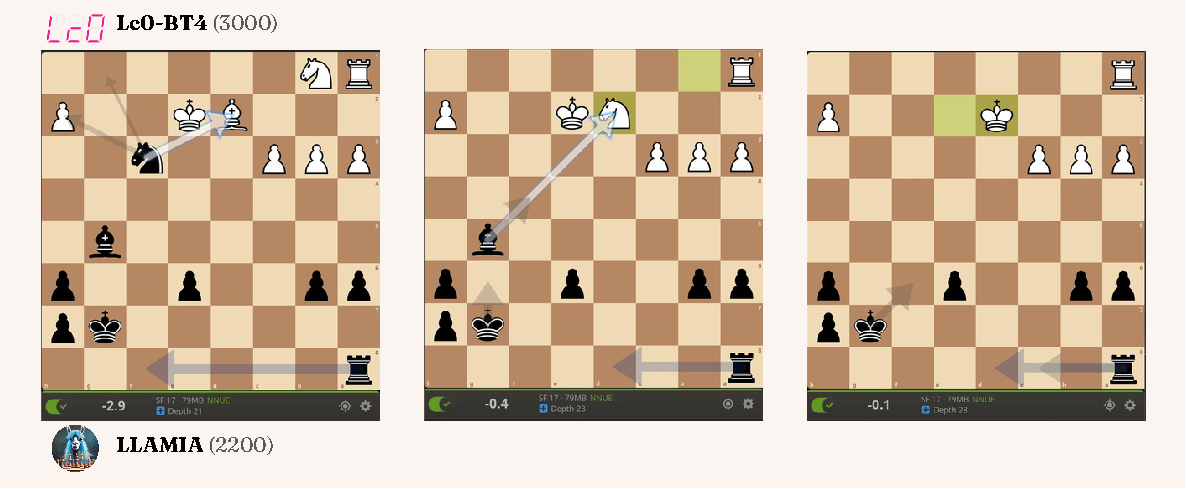
\includegraphics[width=0.95\linewidth]{tcp2.pdf}
    \caption{\textbf{Instruction Conditioned Planning:} LLAMIA is playing against an 800 higher-rated opponent. Note that played moves are indicated with white arrows, and the best moves are shown by blue arrows (size is ordered by the strength of the move). The following instruction is passed: ``your opponent is significantly weaker in endgames''. Orange and yellow moves indicate Mistakes and inaccuracies below. LLAMIA, in this position, plays the move \textbf{\textcolor{orange}{1... Nxd2??}} which is a mistake as it loses its advantage but creates a forced move sequence \textbf{[2. Nxd2 \textcolor{yellow}{Bxd2?} 3. Kxd2]} where it ends with a slightly better position in a rook endgame. Since our task design switches the Elo of Lc0 with a weaker policy here (1500) it ends up winning the game smoothly 19 moves later. LLAMIA was able to plan the forced exchange to trade down in an endgame where it knew it was better, demonstrating its superior planning. \textbf{FEN:[r7/6kp/pp2p2p/6b1/8/PPP2n2/3BK2P/RN6 b - - 0 1]}
}
    \vspace{-3mm}
    \label{fig:tcp}

\end{figure}

\label{app:conditional_planning_eval}
Players exhibit varying strategic strengths and weaknesses across different positional motifs, tactical patterns, and structural imbalances. To evaluate LLAMIA's ability to condition its policy on open-ended natural language directives—e.g., "target opponent’s endgame weaknesses"—we construct a benchmark to test LLAMIA’s ability to exploit such information when provided as a string.

We curate a set of 25 strategic motifs, selected based on: (a) their presence across all skill levels, (b) detectability via automated board heuristics or engine rollouts, and (c) coverage of diverse planning scenarios. Each motif category reflects a distinct type of strategic adaptation. We categorize them as follows:

\begin{enumerate}
    \item \textbf{Endgames:} Detected by material thresholds examples including.
    \begin{itemize}
        \item King and pawn vs. king
        \item Queen endgames
        \item Rook endgames
        \item Opposite-colored bishops
        \item Lucena and Philidor positions
        \item Minor piece vs. pawn endgames
    \end{itemize}
    
    \item \textbf{Pawn Structures:} Detected via relative pawn geometry:
    \begin{itemize}
        \item Isolated pawns
        \item Doubled pawns
        \item Backward pawns
        \item Passed pawns
        \item Pawn chains
        \item Hanging pawns
    \end{itemize}
    
    \item \textbf{Tactical Blunders:} Identified via engine rollouts revealing "only move" sequences leading to significant evaluation shifts (atleast a change of 400 centipawn evaluation):
    \begin{itemize}
        \item Knight Forks
        \item King Pins
        \item Overloaded defenders
        \item Mate in K$(K<5)$
        \item King Security
    \end{itemize}
    
    \item \textbf{Piece Coordination:} Defined via characteristic imbalances or pairwise dynamics:
    \begin{itemize}
        \item Two rooks vs. queen
        \item Knight and bishop vs. rook
        \item Queen and knight vs. queen and bishop
        \item Bishop pair vs. bishop and knight
        \item Rook on open file vs. unconnected rooks
    \end{itemize}
    
    \item \textbf{Repetition Traps:} Detected via rollout parsing for forced threefold repetitions
\end{enumerate}

Each game in the benchmark starts with an instruction (e.g. "Your opponent is signifcantly stronger than you, but has the following weakness ..., plan the moves to reach such positions to win even if it leads to a temporary disadvantage") and is played against a strong engine. If the model succeeds in steering the position toward the instructed motif, the engine is dynamically downgraded to a weaker engine. The win-rate differential serves as a proxy for strategic alignment and planning competence. The initial engine is Lc0-BT4 with search (>2500 ELO), if the weakness is reached we replace it with MAIA-1900 (emulates a 1900 Elo), note that LLAMIA's playing strength is $>2200$, essentially even at a significant disadvantage it can win over an engine rated more than 300 Elo lesser than it.

\begin{table*}[h]
    \centering
    \begin{adjustbox}{max width=1.05\textwidth}
    \begin{tabular}{c|ccccc|c}
    \toprule[1.2pt]
        \textbf{Model} 
        & \makecell{\textbf{End}\\\textbf{games}} 
        & \makecell{\textbf{Pawn}\\\textbf{Structures}} 
        & \makecell{\textbf{Tactical}\\\textbf{Blunders}} 
        & \makecell{\textbf{Piece}\\\textbf{Coordination}} 
        & \textbf{Repetition} 
        & \makecell{\textbf{Overall}\\\textbf{Improvement}} \\ 
    \midrule
        \textbf{ChessGPT-3B} 
        & 1\% & 1\% & 0\% & 0\% & 2\% 
        & 1.3\% \\
        \textbf{ChessGPT-7B} 
        & 2\% & 2\% & 1\% & 1\% & 3\% 
        & 2.5\% \\
        \textbf{ChessGPT-13B} 
        & 4\% & 4\% & 3\% & 3\% & 5\% 
        & 4.6\% \\\midrule
        \textbf{GPT-4o} 
        & 6\% & 7\% & 5\% & 4\% & 8\% 
        & 6.1\% \\
        \textbf{LLaMA-3.1 405B} 
        & 7\% & 8\% & 6\% & 5\% & 9\% 
        & 7.0\% \\
    \midrule
        \textbf{GPT-4o + Lc0 (Tool-Calling)} 
        & 10\% & 11\% & 9\% & 7\% & 12\% 
        & 9.2\% \\
        \textbf{LLaMA-3.1 405B + Lc0 (Tool-Calling)} 
        & \valgood{11.5\%} & 11.5\% & \valgood{11\%} & 7\% & \valgood{13\%} 
        & 10\% \\
    \midrule
        \textbf{LLAMIA-7B LoRA} 
        & 7\% & 8\% & 6\% & 5\% & 9\% 
        & 7.0\% \\
        \textbf{LLAMIA-7B} 
        & 11\% & \valgood{12\%} & 10\% & \valgood{8\%} & \valgood{13\%} 
        & \valgood{14\%} \\
        \textbf{LLAMIA-13B LoRA} 
        & 8\% & 9\% & 7\% & 6\% & 10\% 
        & 8.0\% \\
        \textbf{LLAMIA-13B} 
        & \valbest{17\%} & \valbest{19\%} & \valbest{14\%} & \valbest{11\%} & \valbest{20\%} 
        & \valbest{17\%} \\
    \bottomrule[1.2pt]
    \end{tabular}
    \end{adjustbox}
    \caption{
\textbf{LLAMIA-Bench Instruct-Conditioned Planning.}  
We evaluate whether models can adapt their strategy in response to explicit instructions about opponent weaknesses an ability crucial for flexible, human-aligned planning. This benchmark measures win-rate improvement when the model is informed that its opponent is vulnerable in specific areas, such as \emph{endgames}, \emph{pawn structure}, or \emph{tactical oversight}. Models play against a stronger engine; if they steer the game into the designated weakness domain, the engine is swapped with a weaker version, allowing the model to capitalize on its plan. While traditional engines (e.g., Stockfish, Lc0) remain invariant and show no improvement (0\%), and large tool-augmented models like GPT-4o + Lc0 achieve moderate gains (9–11\%), LLAMIA-13B delivers the strongest adaptation with a 16.2\% average win-rate gain across five weakness categories. Notably, smaller LoRA-adapted LLAMIA variants outperform much larger LLMs, demonstrating that internalizing structured planning signals via latent-state projection leads to more efficient and interpretable adaptation than external tool-calling or scale alone. Detailed evaluation setup is describe in \cref{app:conditional_planning_eval} \textbf{Overall Improvement} is the weighted average win rate over the subtasks. 
}

    \label{tab:instruct_conditioned_planning}
\end{table*}



% \begin{figure}[!h]
%     \centering
%     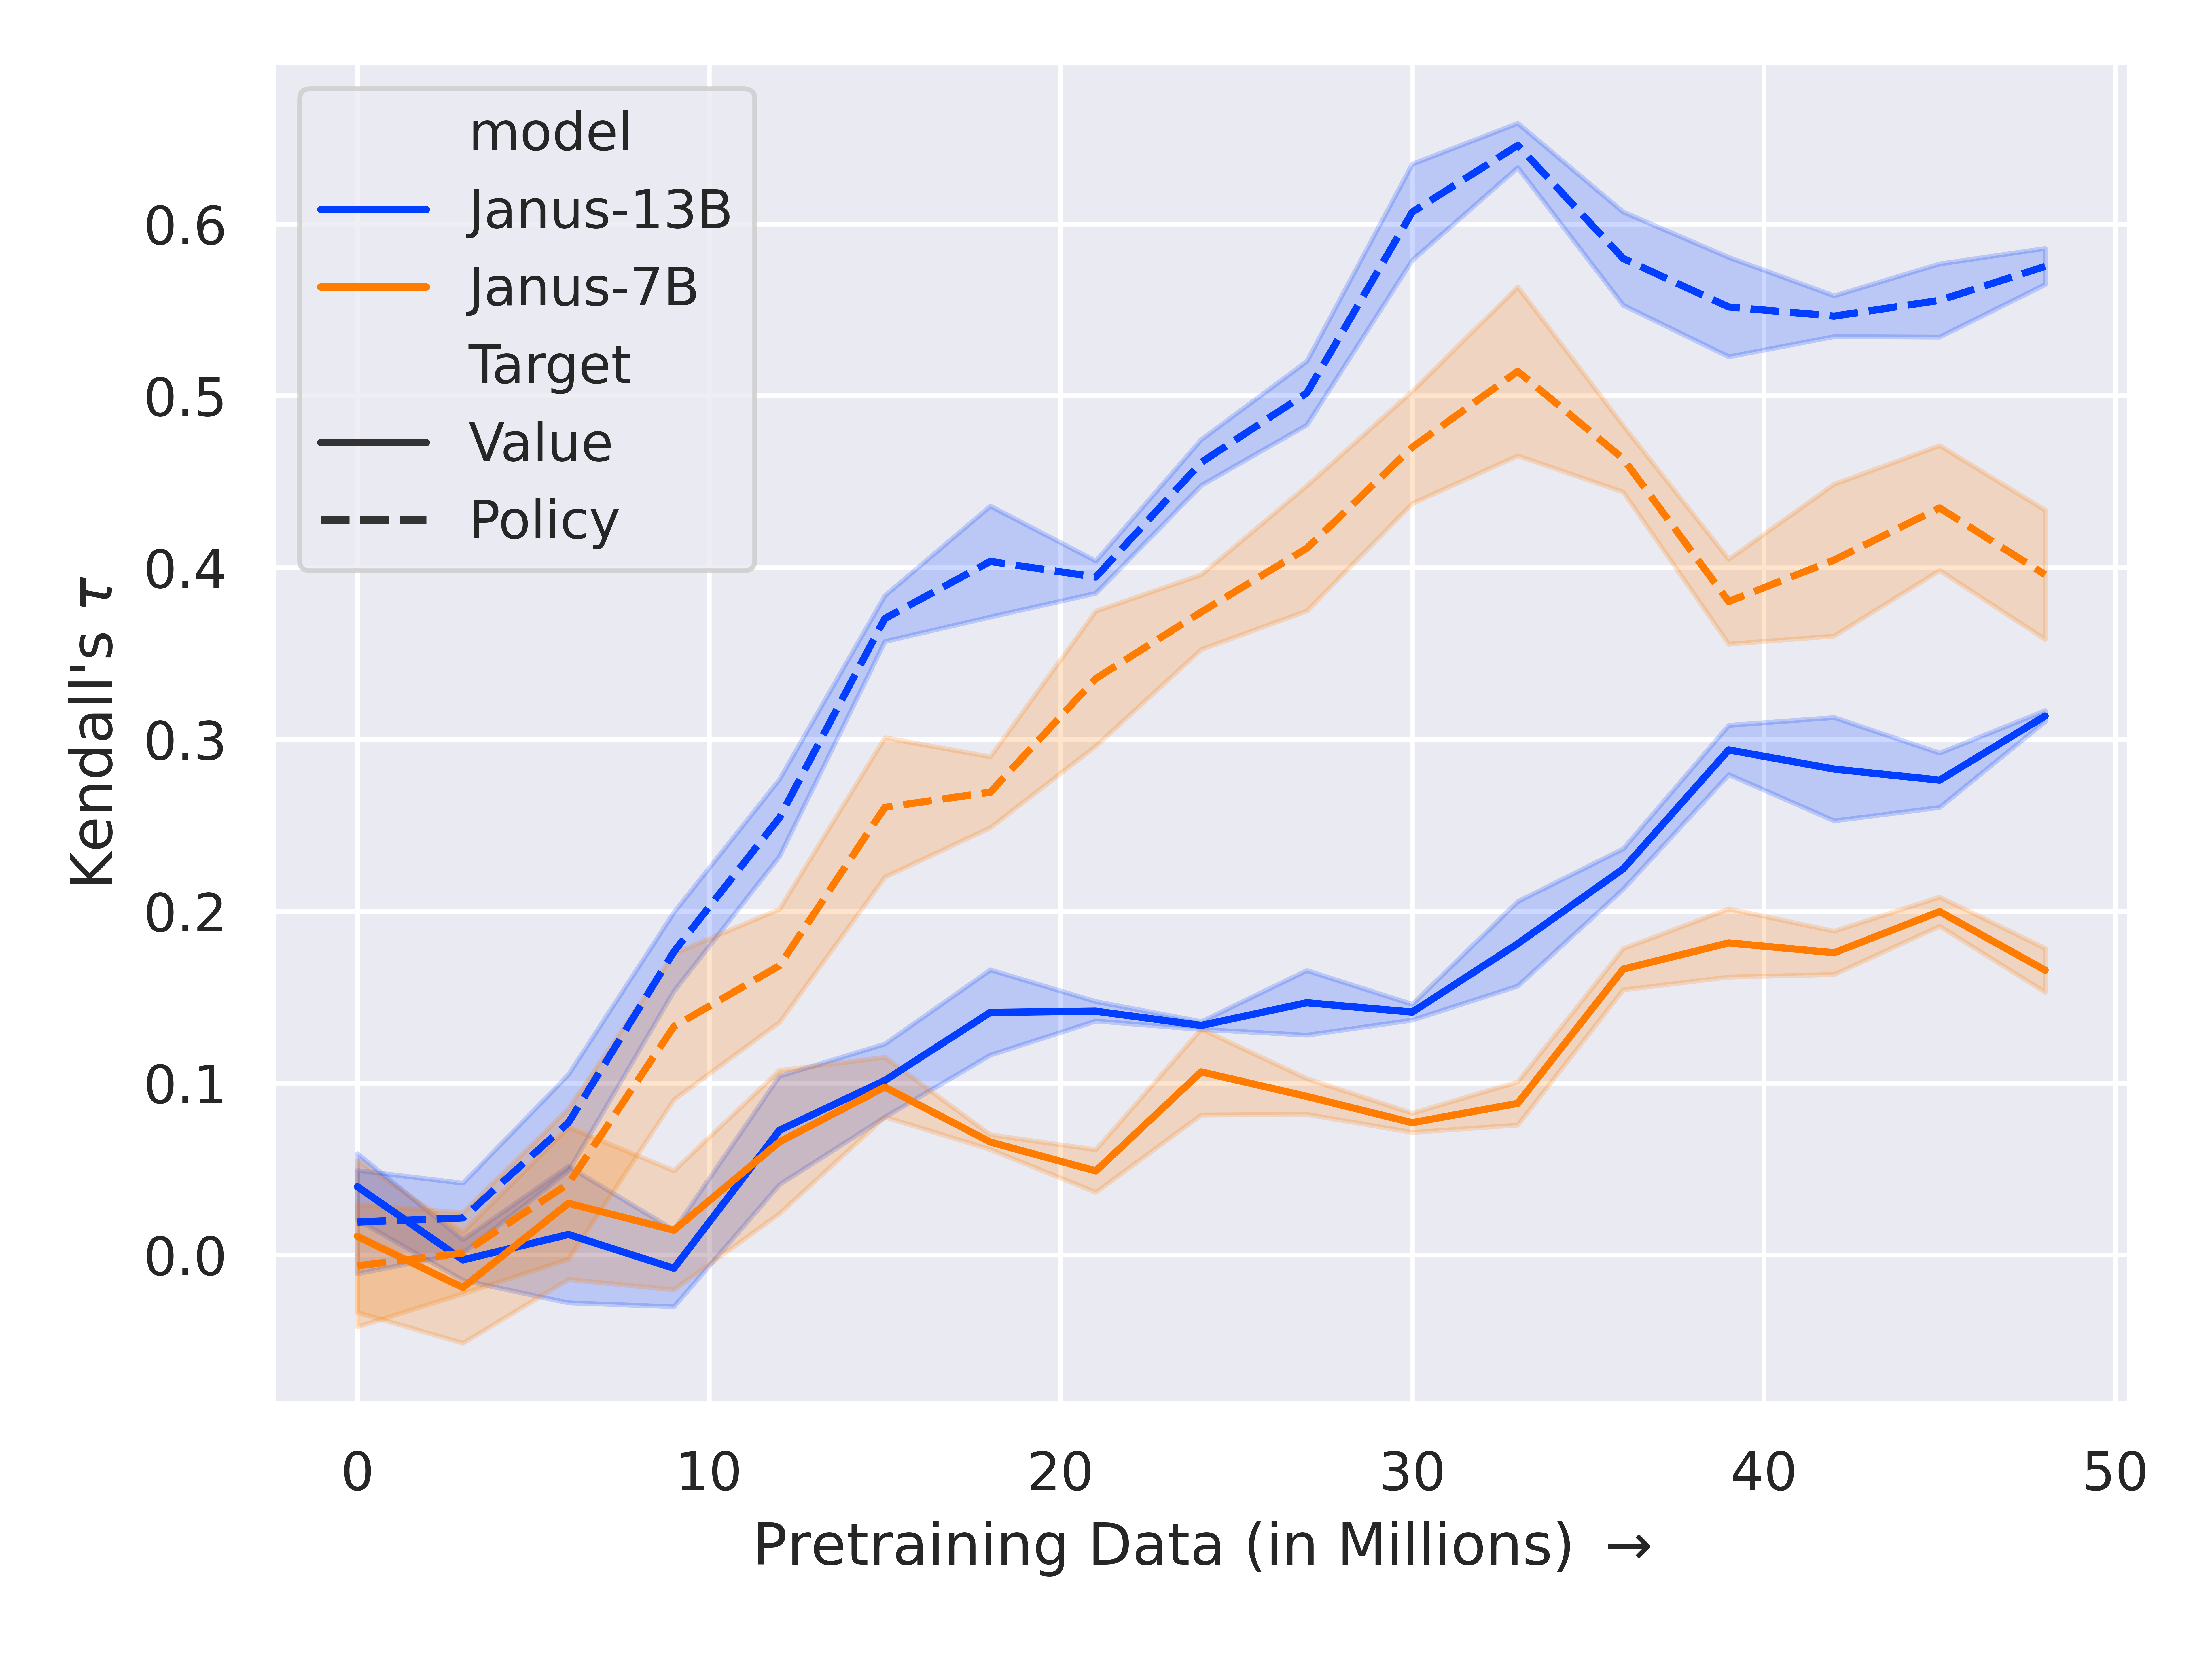
\includegraphics[width=\linewidth]{KendalTau_Alignment.png}
%     \vspace{-8mm}
%     \caption{\textbf{Kendall-$\tau$ alignment} scaling with data and parameters. The alignment between the LLM's policy and Agent's Value (Q-values post search) and Policy (Base policy). Over 30 million points the alignment with both policy and value improves, interestingly both 13B and 7B models exhibit an area (30M-40M) where they start deviating from policy to value, we call this the shallow ``internal search''}.
%     \label{fig:pretraining-curve}
% \end{figure}
\subsection{Environment Extension}
To evaluate the extensibility of our framework we extend our approach to two new tasks, \textbf{Text-to-Image Preference Alignment} to predict and improve alignment of image generation models and goal directed language through \textbf{PersuasionBench}. We follow the exact same setup, training data, and evaluation protocol as \cite{xu2025visionrewardfinegrainedmultidimensionalhuman} and \cite{singh2024measuring}.

\begin{table*}[h]
    \centering
    \begin{adjustbox}{max width=1.05\textwidth}
    \begin{tabular}{l|c|cccc|c}
    \toprule[1.2pt]
    \textbf{Model} & \textbf{Method} & \textbf{Composition} & \textbf{Quality} & \textbf{Fidelity} & \textbf{Emotion} & \textbf{HPDv2 (Tau*)} \\
    \midrule
    GPT-4o & ICL & 73.1 & 62.7 & 61.9 & 70.1 & 77.5 \\
    Gemini & ICL & 69.4 & 59.9 & 59.7 & 74.9 & 60.7 \\
    CogVLM2 & ICL & 65.8 & 67.1 & 53.1 & 74.7 & 64.5 \\
    LLaVA & ICL & 59.9 & 65.7 & 59.8 & 64.4 & 61.0 \\
    VisionReward-19B & IFT & \valbest{78.8} & \valgood{81.1} & \valgood{80.9} & \valgood{83.9} & \valgood{81.7} \\
    GPT-4o + ImageReward & ICL + ToolCalling & 75.5 & 65.0 & 64.0 & 72.5 & 79.5 \\
    \midrule
    LLAMIA-19B (Ours) & SALT & \valgood{76.5} & \valbest{85.0} & \valbest{82.0} & \valbest{84.2} & \valbest{85.8} \\
    \bottomrule[1.2pt]
    \end{tabular}
    \end{adjustbox}
    \caption{\textbf{Image Generation Evaluation.} We evaluate LLAMIA-13B and prior vision-language models across perceptual axes (composition, quality, fidelity, emotion) from VisionReward \cite{xu2025visionrewardfinegrainedmultidimensionalhuman} and preference alignment via HPDv2\cite{wu2023human}. Despite having the same underlying base VLM (CogVLM2-llama3-chat\cite{hong2024cogvlm2}) LLAMIA internally integrates ImageReward\cite{xu2023imagereward} and outperforms all baselines in HPDv2 alignment (\valbest{85.7}), improving over GPT-4o (\valgood{77.5}) by \textbf{+8.2} and over VisionReward by \textbf{+4.1} with the same amount of training data for this task. We follow the same evaluation as \cite{xu2025visionrewardfinegrainedmultidimensionalhuman} However due to unavailability of Monet-Bench we could not include it.}
    \label{tab:image_generation}
\end{table*}

\begin{table}[!h]
\centering
\adjustbox{max width=0.95\textwidth}{
\begin{tabular}{l|c|c|c|c}
\toprule[1.2pt]
\textbf{Model} & \textbf{Size} & \textbf{Method} & \textbf{\makecell{Behavior\\Simulation}} & \textbf{\makecell{Comparative\\Transsuasion}} \\
\midrule
GPT-4o & * & ICL & 43.2 & 57.3 \\
GPT-4 & * & ICL & 39.2 & 55.7 \\
GPT-3.5 & * & ICL & 35.6 & 50.6 \\
LLaMA-3-70B & 70B & ICL & 37.4 & 52.6 \\
\midrule
Transsuasion-13B & 13B & IFT & 59.8 & 77.0 \\
\midrule
LLAMIA (Self-only) & 13B & SALT & \valgood{61.0} & 77.5 \\
LLAMIA (Industry-only) & 13B & SALT & 60.1 & \valgood{79.2} \\
LLAMIA (Self \& Industry) & 13B & SALT & \valbest{63.4} & \valbest{80.1} \\
\bottomrule
\end{tabular}}
\vspace{2mm}
\caption{\textbf{Simulative Persuasion Performance on PersuasionBench.} 
We evaluate models on behavior simulation (BS) predicting tweet engagement levels and comparative transsuasion (TS) choosing the more engaging of two tweets. LLAMIA outperforms all baselines with a \textbf{6\% gain} in BS and \textbf{4\% in TS} over Transsuasion-13B, despite using only 50\% of the training data. LLAMIA internalizes a time-series critic, \texttt{chronos-bolt-base}\cite{ansari2024chronos}, trained to forecast engagement trends over a 14-day horizon using both post-author (self) and brand-level (industry) temporal signals. Ablations show that self-only and industry-only variants individually improve over the IFT baseline, but their combination yields the best generalization. This highlights the synergistic benefit of modeling both personalized and group-level engagement dynamics within the SALT framework.}
\label{tab:persuasion_llamia}
\end{table}


\begin{figure}[!h]
    \centering
    \includegraphics[width=\linewidth]{aesth (2).pdf}
    \vspace{-2mm}
    \caption{
\textbf{Qualitative Examples: Image Preference Alignment via Internalized Rewards.}  
We compare images generated using VisionReward (left), LLAMIA-ImageReward (middle), and human-preferred selections (right) across diverse prompts involving aesthetic composition, product photography, and stylistic variation. LLAMIA-ImageReward yields more coherent framing, superior lighting consistency, and better adherence to prompt-specific constraints, as also reflected in human preference studies (+5 pp). Notably, these improvements emerge with half the fine-tuning data, demonstrating LLAMIA’s capacity to internalize domain-specific reward functions and generalize stylistic priors across prompts.
}.
    \label{fig:image_grid}
\end{figure}
\FloatBarrier

\begin{figure}[htbp]
    \centering
    \begin{subfigure}[b]{0.5\linewidth}
        \centering
        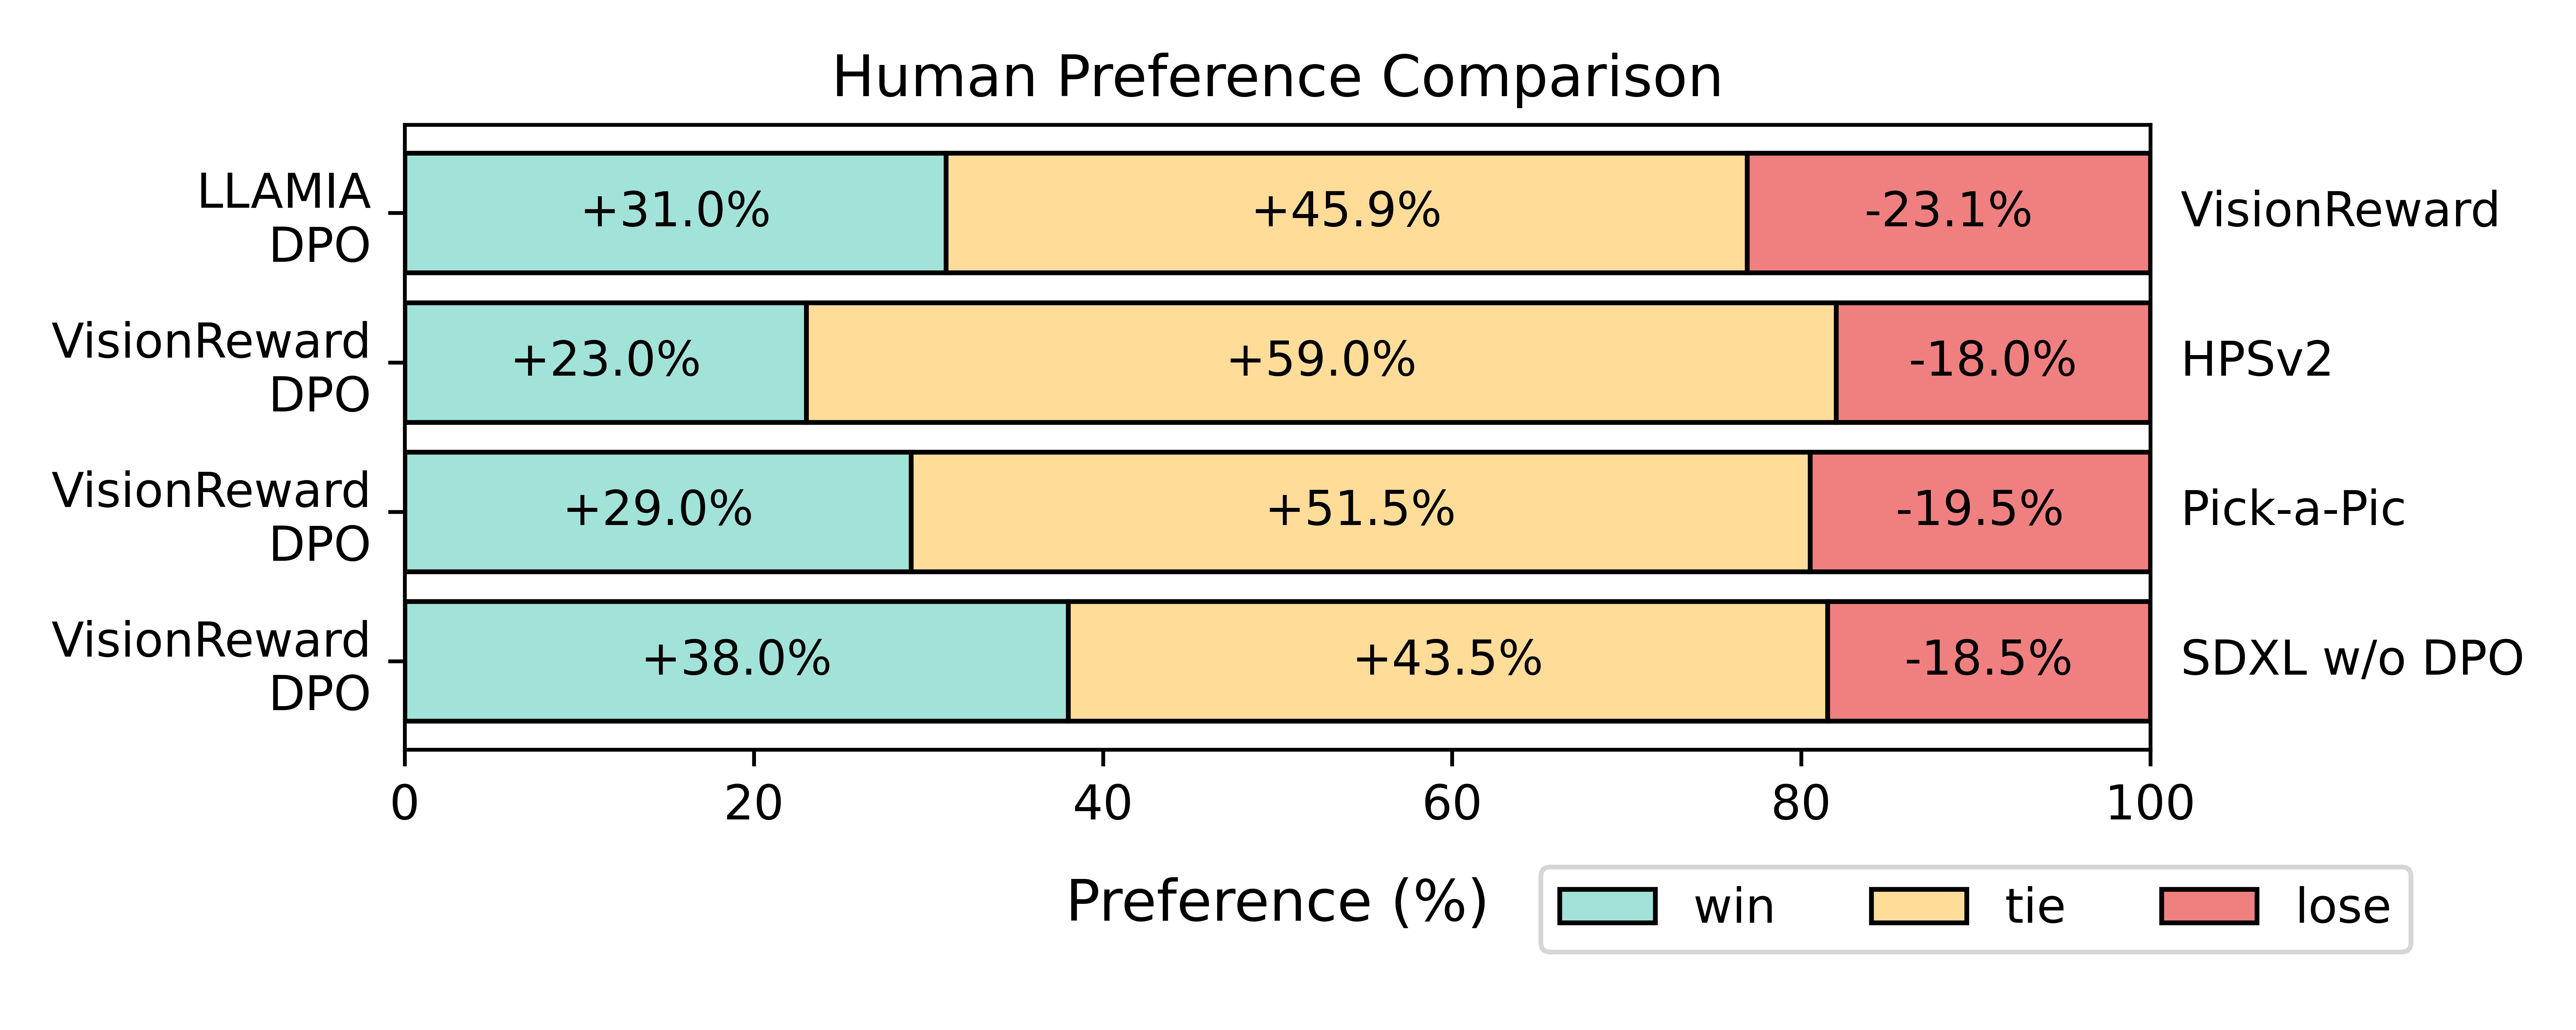
\includegraphics[width=\linewidth]{human_preference_comparison.png}
        \caption{\textbf{Human Preference Comparison:} Human raters prefer LLAMIA’s SDXL generations over VisionReward’s by a margin of +7.9\%. While VisionReward improves significantly over raw SDXL (e.g., +19.5\% win rate), LLAMIA’s internal reward alignment improves sample-level aesthetics and relevance further, as reflected in Pick-a-Pic and HPSv2 gains.}
        \label{fig:subfig-human-preference}
    \end{subfigure}
    \hfill
    \begin{subfigure}[b]{0.48\linewidth}
        \centering
        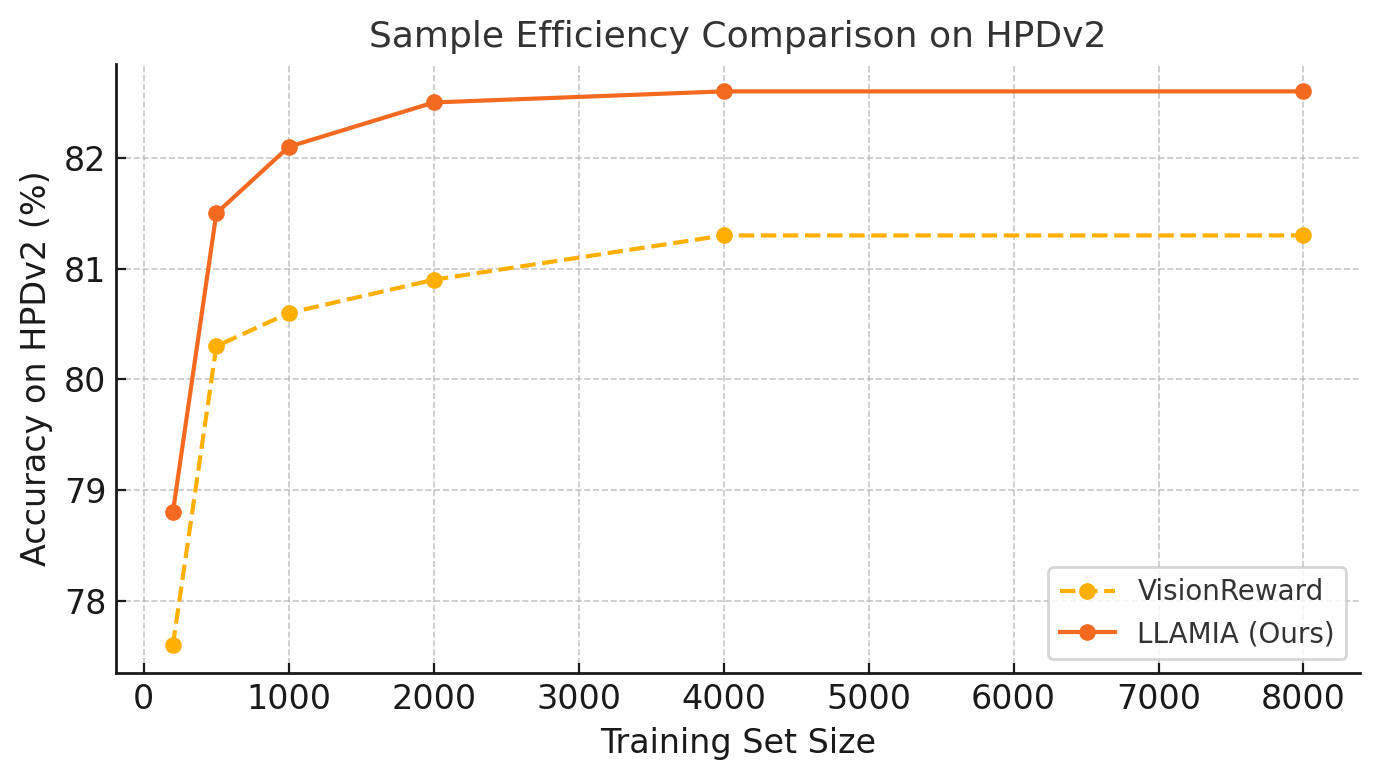
\includegraphics[width=\linewidth]{output (7).png}
        \caption{\textbf{Sample Efficiency on HPDv2:} LLAMIA shows significantly better sample efficiency over VisionReward on the HPDv2 benchmark. It achieves 81.3\% accuracy with just 2k samples, matching VisionReward’s peak accuracy with 8k samples. This highlights that internalizing ImageReward within the generation process yields more data-efficient preference modeling.}
        \label{fig:subfig-model-output}
    \end{subfigure}
\caption{\textbf{Quantitative Analysis of Visual Reward Alignment.} We compare LLAMIA to VisionReward across two axes: (a) sample efficiency of preference prediction and (b) human preference studies on DPO-enhanced SDXL generations. LLAMIA consistently achieves higher accuracy and win rates with fewer samples.}
    \label{fig:comparison}
\end{figure}

\clearpage
\section{Prompt listings}
\subsection{Pretraining}
\label{listing:pretraining_instruction_format}
      
\begin{tcolorbox}[
  colback=white,
  colframe=black!75!white,
  colbacktitle=black!75!white,
  title=Pretraining instruction format,
  enhanced,
  before upper={% Insert the figure at the top-left
    \begin{minipage}{0.3\textwidth} % Adjust width as needed
      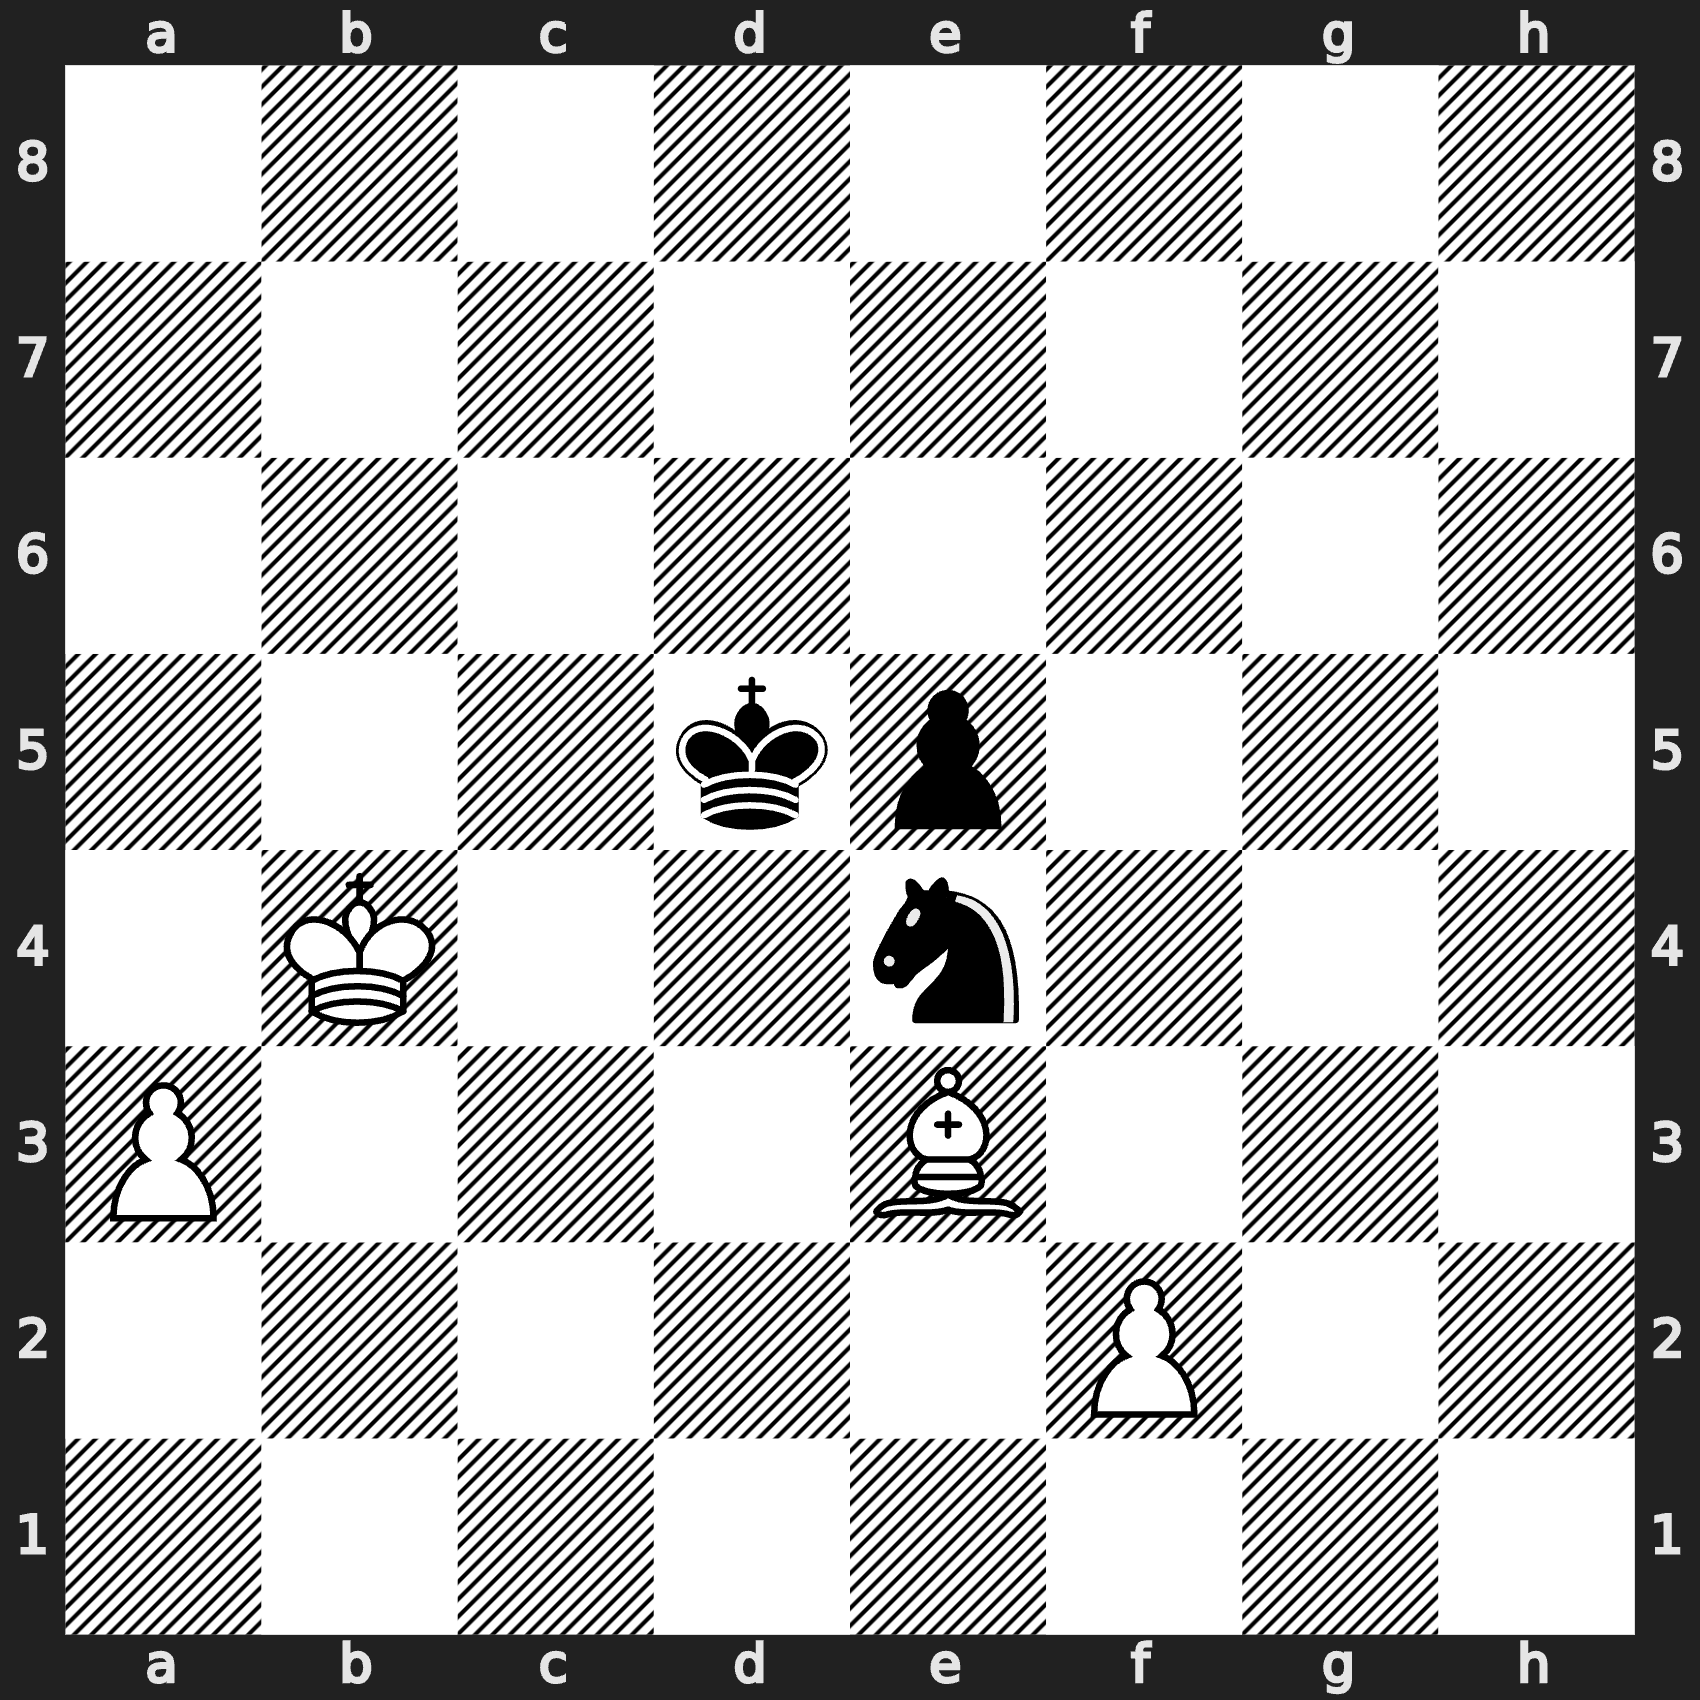
\includegraphics[width=\textwidth]{boards/pretrain_board.png}
    \end{minipage}\\[10pt]
  }
]
FEN: \textbf{8/8/8/3kp3/1K2n3/P3B3/5P2/8 b - - 0 1} \\ \\
\textbf{Human}
\texttt{<state>}
What is the evaluation of the following position? Describe the evaluation followed by the continuation in UCI format e.g. if the evaluation is +1.5 and the best continuation is e2e4 e7e5, you should write "Evaluation is +1.5, Advantage for White, e2e4 e7e5"

\tcbline
\textbf{LLAMIA} \\
Evaluation is +0.5, white has a slight advantage, d5c6 b4c4 e4d6 c4d3 d6e8 d3e4 e8d6 e4d3 c6d5

\tcbline
\textbf{Human} \\
Give me the principal variation(s), just give me the evaluation(s) and the line(s)

\tcbline
\textbf{LLAMIA} \\
+0.4, e4d6 a3a4 d5c6 b4c3 c6d5 c3d3

\tcbline
\textbf{Human} \\
What are the legal moves in this position? Give me up to 10 comma-separated UCI moves and nothing else

\tcbline
\textbf{LLAMIA} \\
e4f2 d5e6 e4c3 e4g3 e4d6 e4g5 e4d2 e4f6 d5d6 e4c5

\tcbline
\textbf{Human} \\
Describe the current position briefly

\tcbline
\textbf{LLAMIA} \\
It is black's turn, the current position is: \\
- White's King is somewhat exposed, with threats from Black's Knight and Pawn.\\
- Black has a centralized active Knight and Pawn.\\
- Both sides have pawns on the board but White has a central pawn that could potentially become mobile.\\
This position appears as a complex endgame with white on slight advantage due to their extra pawn.
\end{tcolorbox}
\vspace{-3mm}
% \captionof{figure}{\textbf{Pre-training Instruction Format:} We use SAN and UCI move notations with 30/70 probabilities, all evaluations are in pawn evaluations. The legal moves are automatically generated based on the UCI protocol and position description is generated using LLaMA-405B from feature verbalizations }

\subsection{Puzzles}
\label{listing:puzzle_instruction_format}
\begin{tcolorbox}[
  colback=white,
  colframe=black!75!white,
  colbacktitle=black!75!white,
  title=Puzzle instruction,
  enhanced,
  before upper={% Insert the figure at the top-left
    \begin{minipage}{0.3\textwidth} % Adjust width as needed
      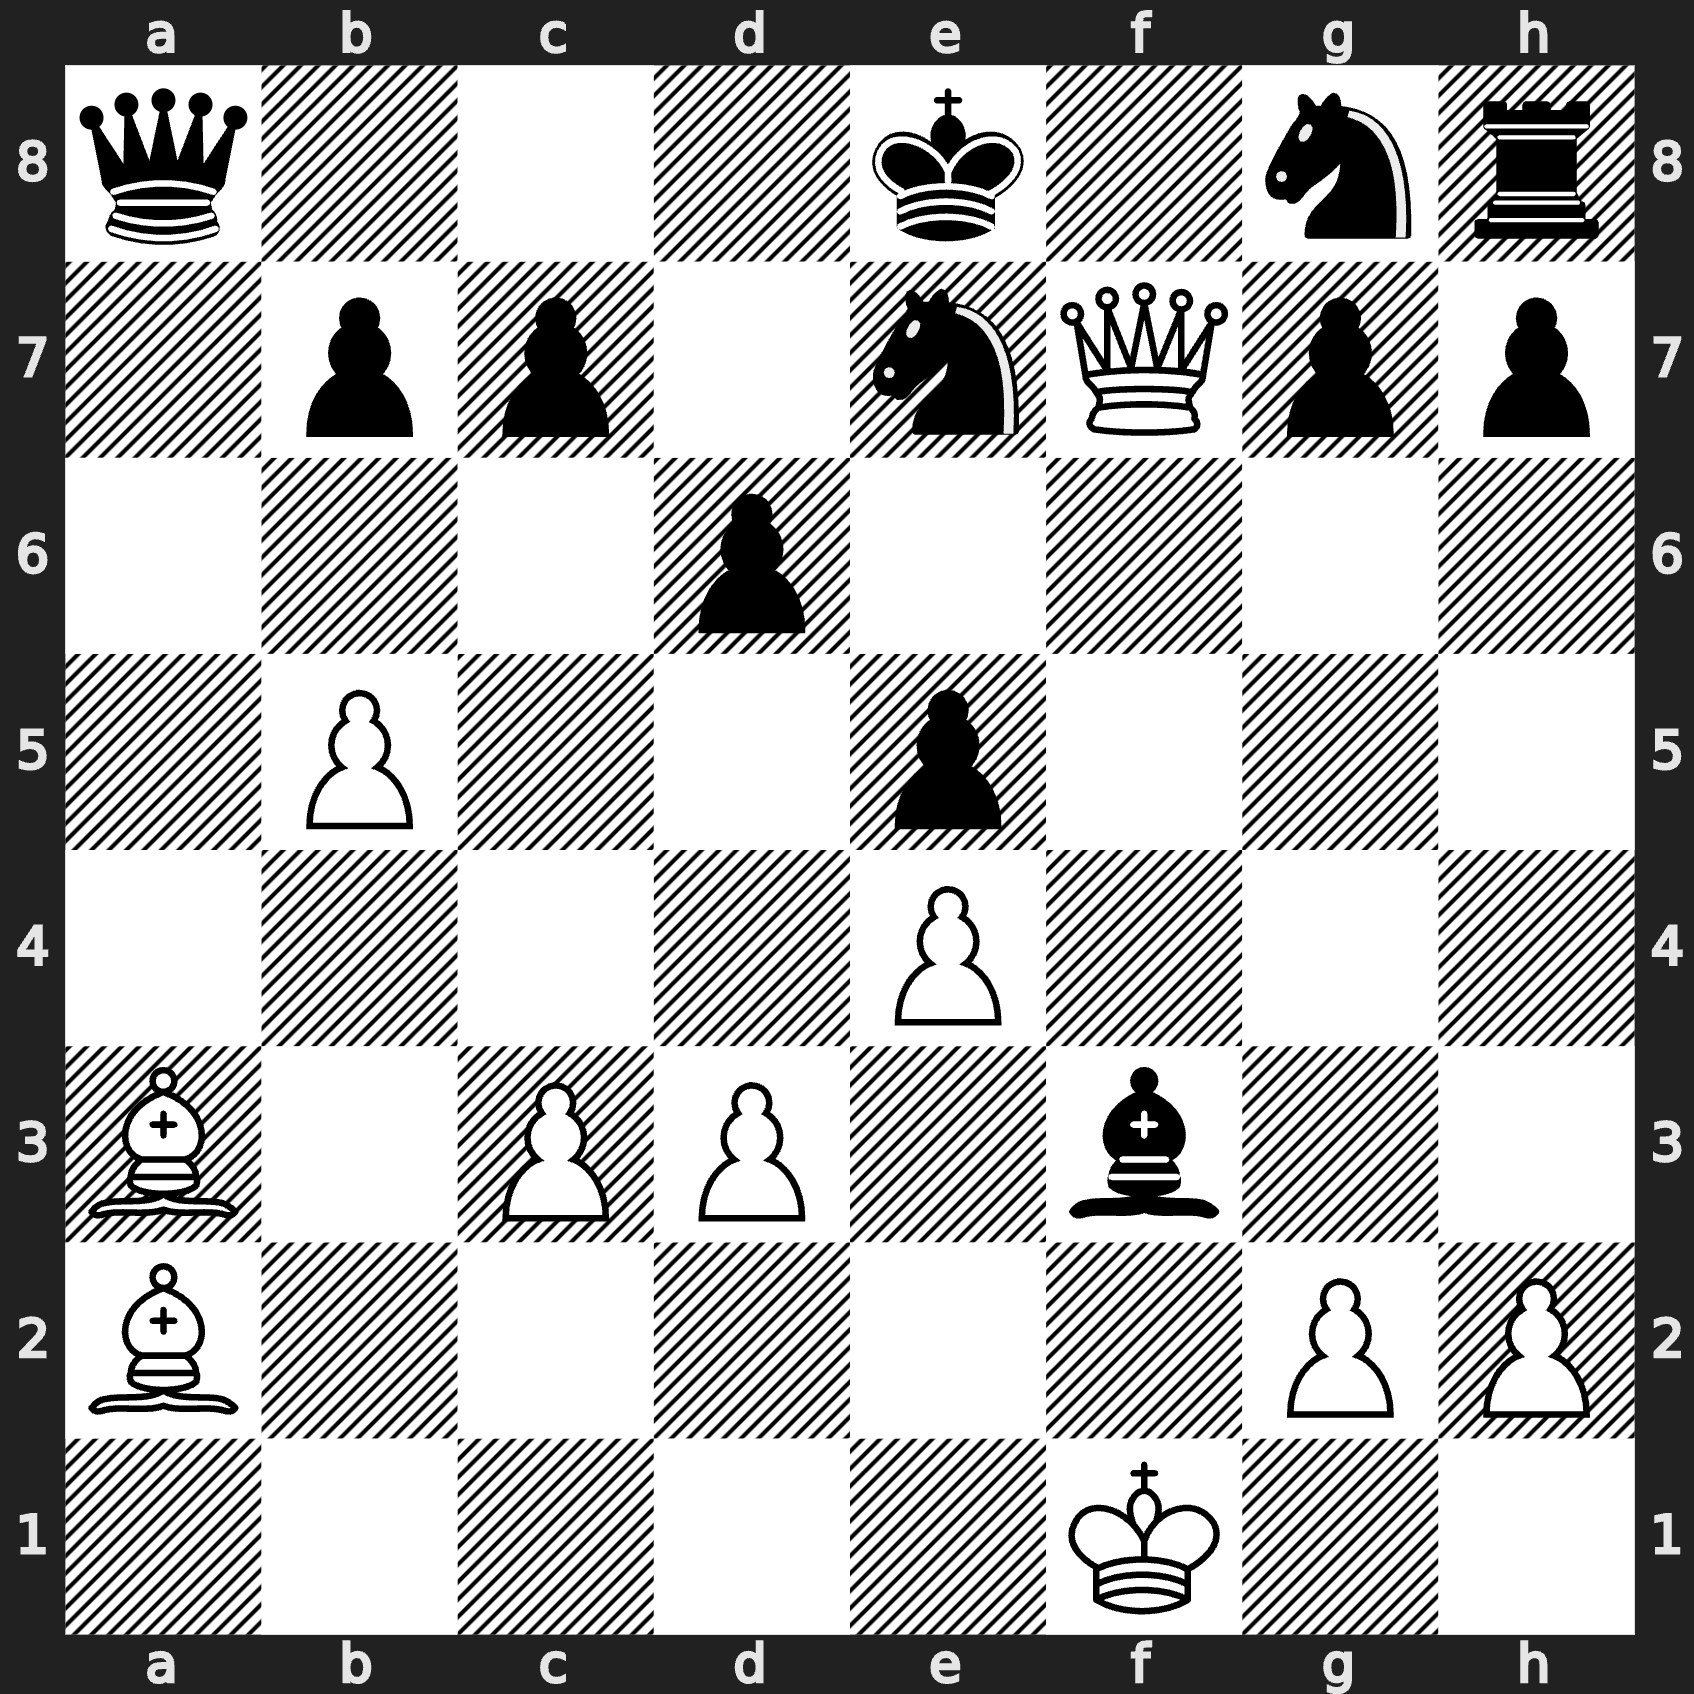
\includegraphics[width=\textwidth]{1.png}
      
    \end{minipage}\\[10pt]
  }
]
FEN: \textbf{q3k1nr/1pp1nQpp/3p4/1P2p3/4P3/B1PP1b2/B5PP/5K2 b k - 0 17}
\tcbline
\textbf{Human} \\
Your task is to describe and then solve the given puzzle \texttt{<state>}.
What are the themes for this puzzle? Only give me the comma separated themes and nothing else.

\tcbline
\textbf{LLAMIA} \\
mate, mateIn2, middlegame, short

\tcbline
\textbf{Human} \\
What is the solution to the puzzle? Answer must be in UCI notation.

\tcbline
\textbf{LLAMIA} \\
e8d7 a2e6 d7d8 f7f8

\tcbline
\textbf{Human} \\
What would be the popularity and the Elo of the puzzle. Popularity is a number between 100 (best) and -100 (worst).

\tcbline
\textbf{LLAMIA} \\
The popularity is 88 and the Elo is 1904
\end{tcolorbox}

\noindent\begin{minipage}{0.5\textwidth}
\vspace{-10pt}
% \captionof{figure}{\textbf{Puzzle Instruction Format}}

\end{minipage}

\subsection{Behavior Cloning}

\begin{tcolorbox}[
  colback=white,
  colframe=black!75!white,
  colbacktitle=black!75!white,
  title=CCRL instruction,
  enhanced,
  before upper={% Insert the figure at the top-left
    \begin{minipage}{0.3\textwidth} % Adjust width as needed
      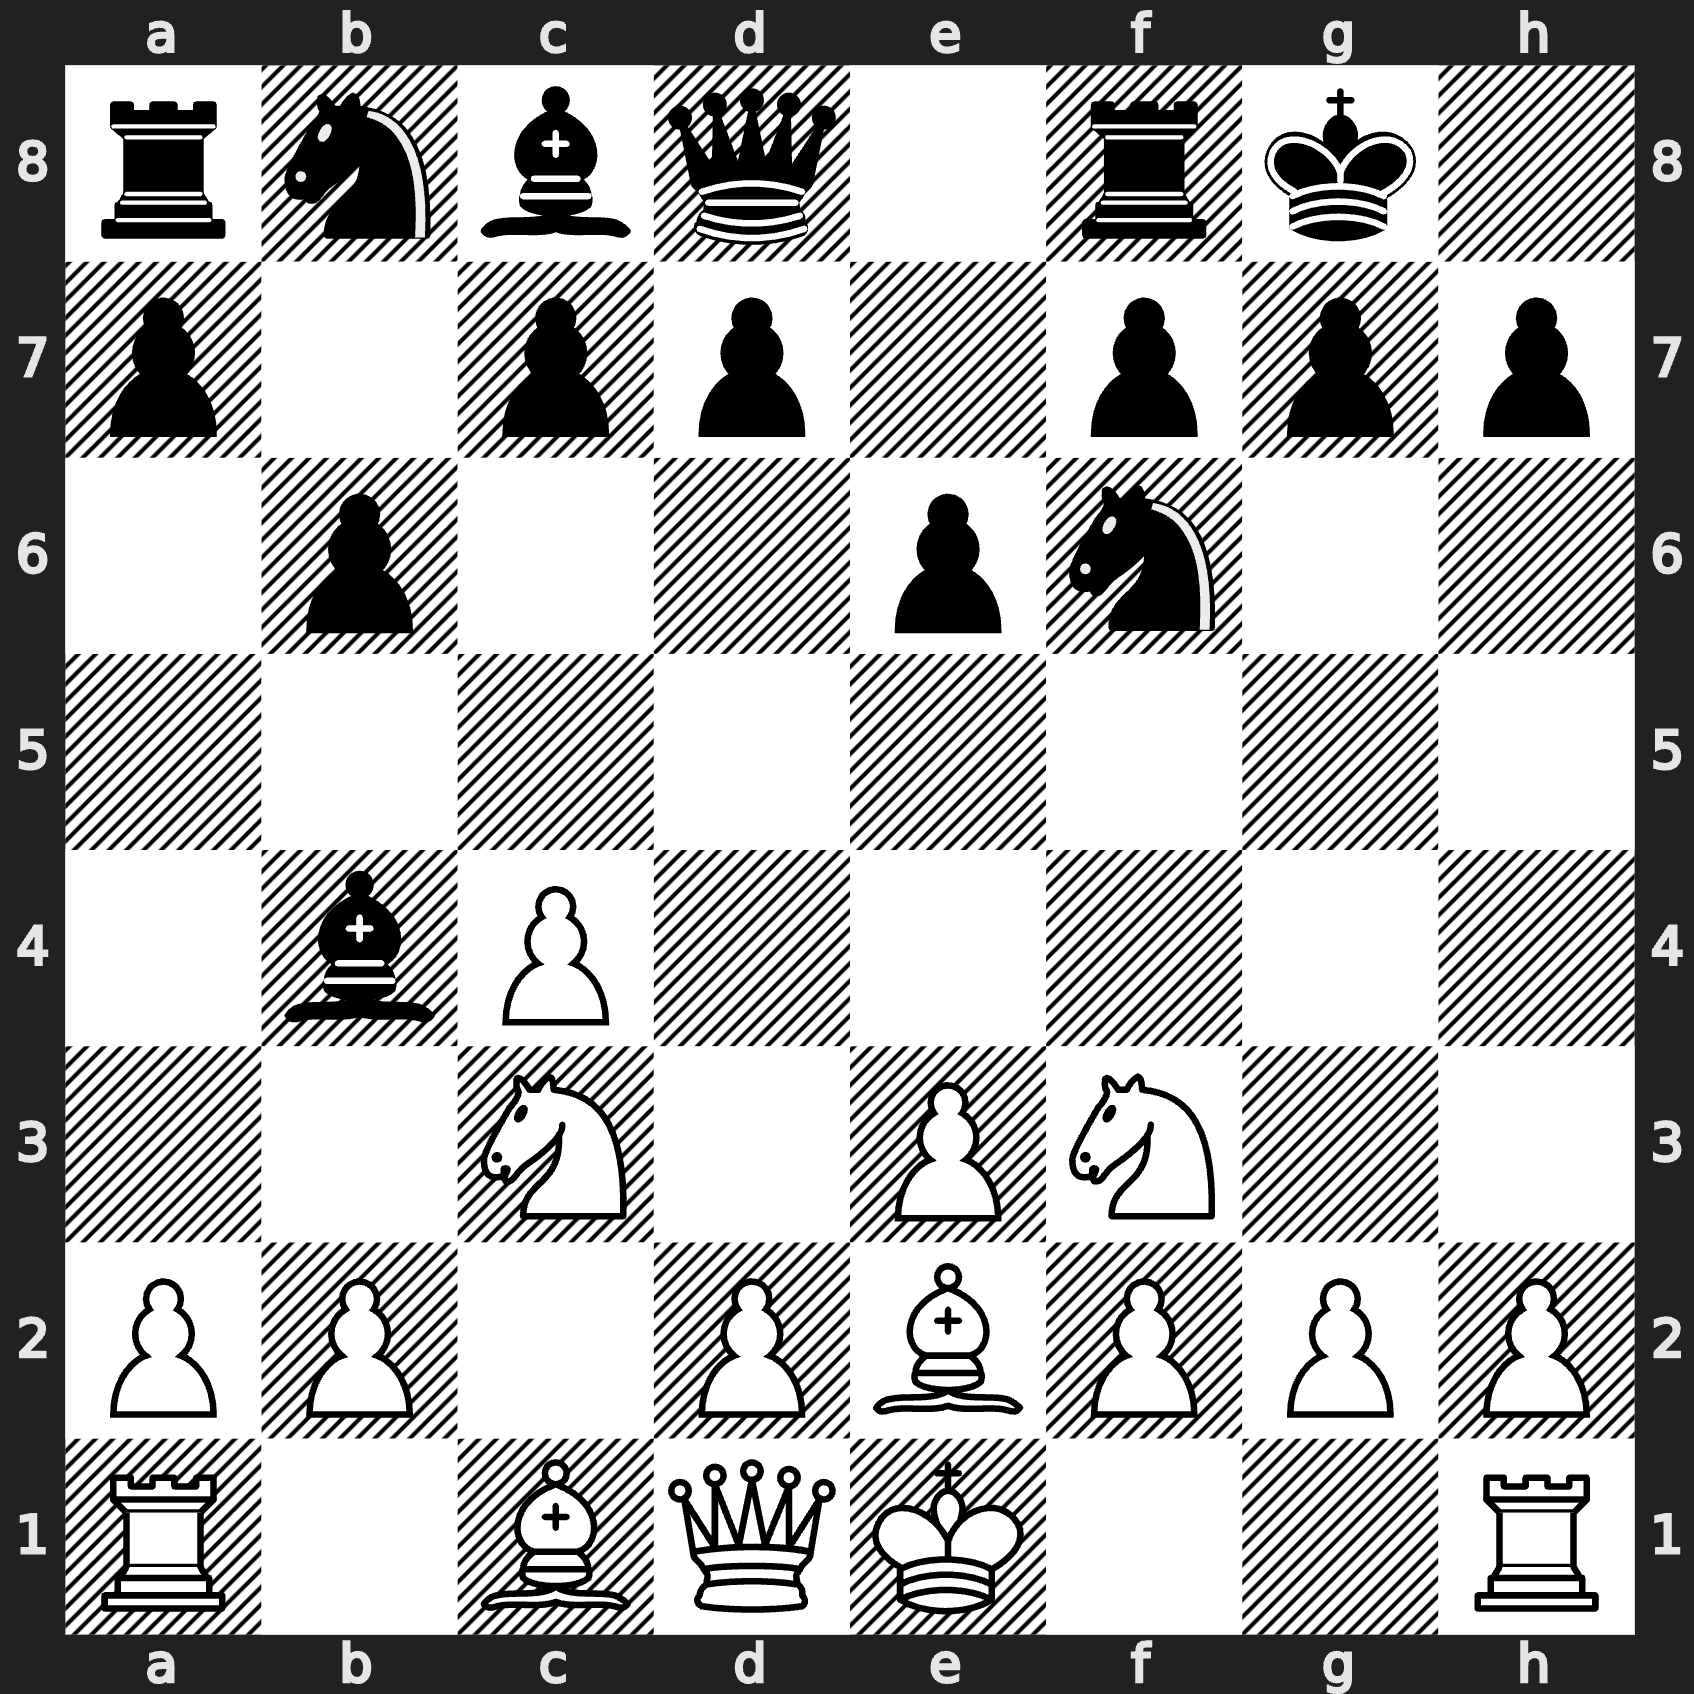
\includegraphics[width=\textwidth]{2.png}
  
    \end{minipage}\\[10pt]
  }
]
FEN: \textbf{rnbq1rk1/p1pp1ppp/1p2pn2/8/1bP5/2N1PN2/PP1PBPPP/R1BQK2R w KQ - 0 6}
\tcbline
\textbf{Human} \\
You have to simulate the following game: \\
Engine (2754) - Engine (2710)\\
Rating Difference = 44\\
Event: Computer Chess Rating List 40/15\\
ECO: A17\\
Opening: English\\
Variation: Nimzo-English opening\\
The last 3 moves were e8g8 f1e2 b7b6 \texttt{<state>}\\
Analyze the position and predict what would be the next 9 moves. Provide your response as a list of UCI moves.

\tcbline
\textbf{LLAMIA} \\
The next moves are: e1g1 c8b7 d2d4 d7d6 c1d2 b8d7 c3b5 b4d2 f3d2

\tcbline
\textbf{Human} \\
The last 3 moves were f3d2 e6e5 d1c2 \texttt{<state>}\\
Analyze the position and predict what would be the next 5 moves.

\tcbline
\textbf{LLAMIA} \\
The next moves are: a7a6 b5c3 d8e7 d4d5 a8e8

\tcbline
\textbf{Human} \\
The last move was a2a3 \texttt{<state>}\\
Analyze the position and predict what would be the next 3 moves.

\tcbline
\textbf{LLAMIA} \\
The next moves are: f8e8 f1e1 d7f8

\tcbline
\textbf{Human} \\
The last move was d2f1 \texttt{<state>}\\
Analyze the position and predict what would be the next 8 moves.

\tcbline
\textbf{LLAMIA} \\
The next moves are: h6h5 f1e3 b7c8 e2f3 h5h4 c2d2 h4h3 e3f5
\label{listing:ccrl_instruction_format}
\end{tcolorbox}

\begin{tcolorbox}[
  colback=white,
  colframe=black!75!white,
  colbacktitle=black!75!white,
  title=Lichess instruction,
  enhanced,
  before upper={% Insert the figure at the top-left
    \begin{minipage}{0.3\textwidth} % Adjust width as needed
      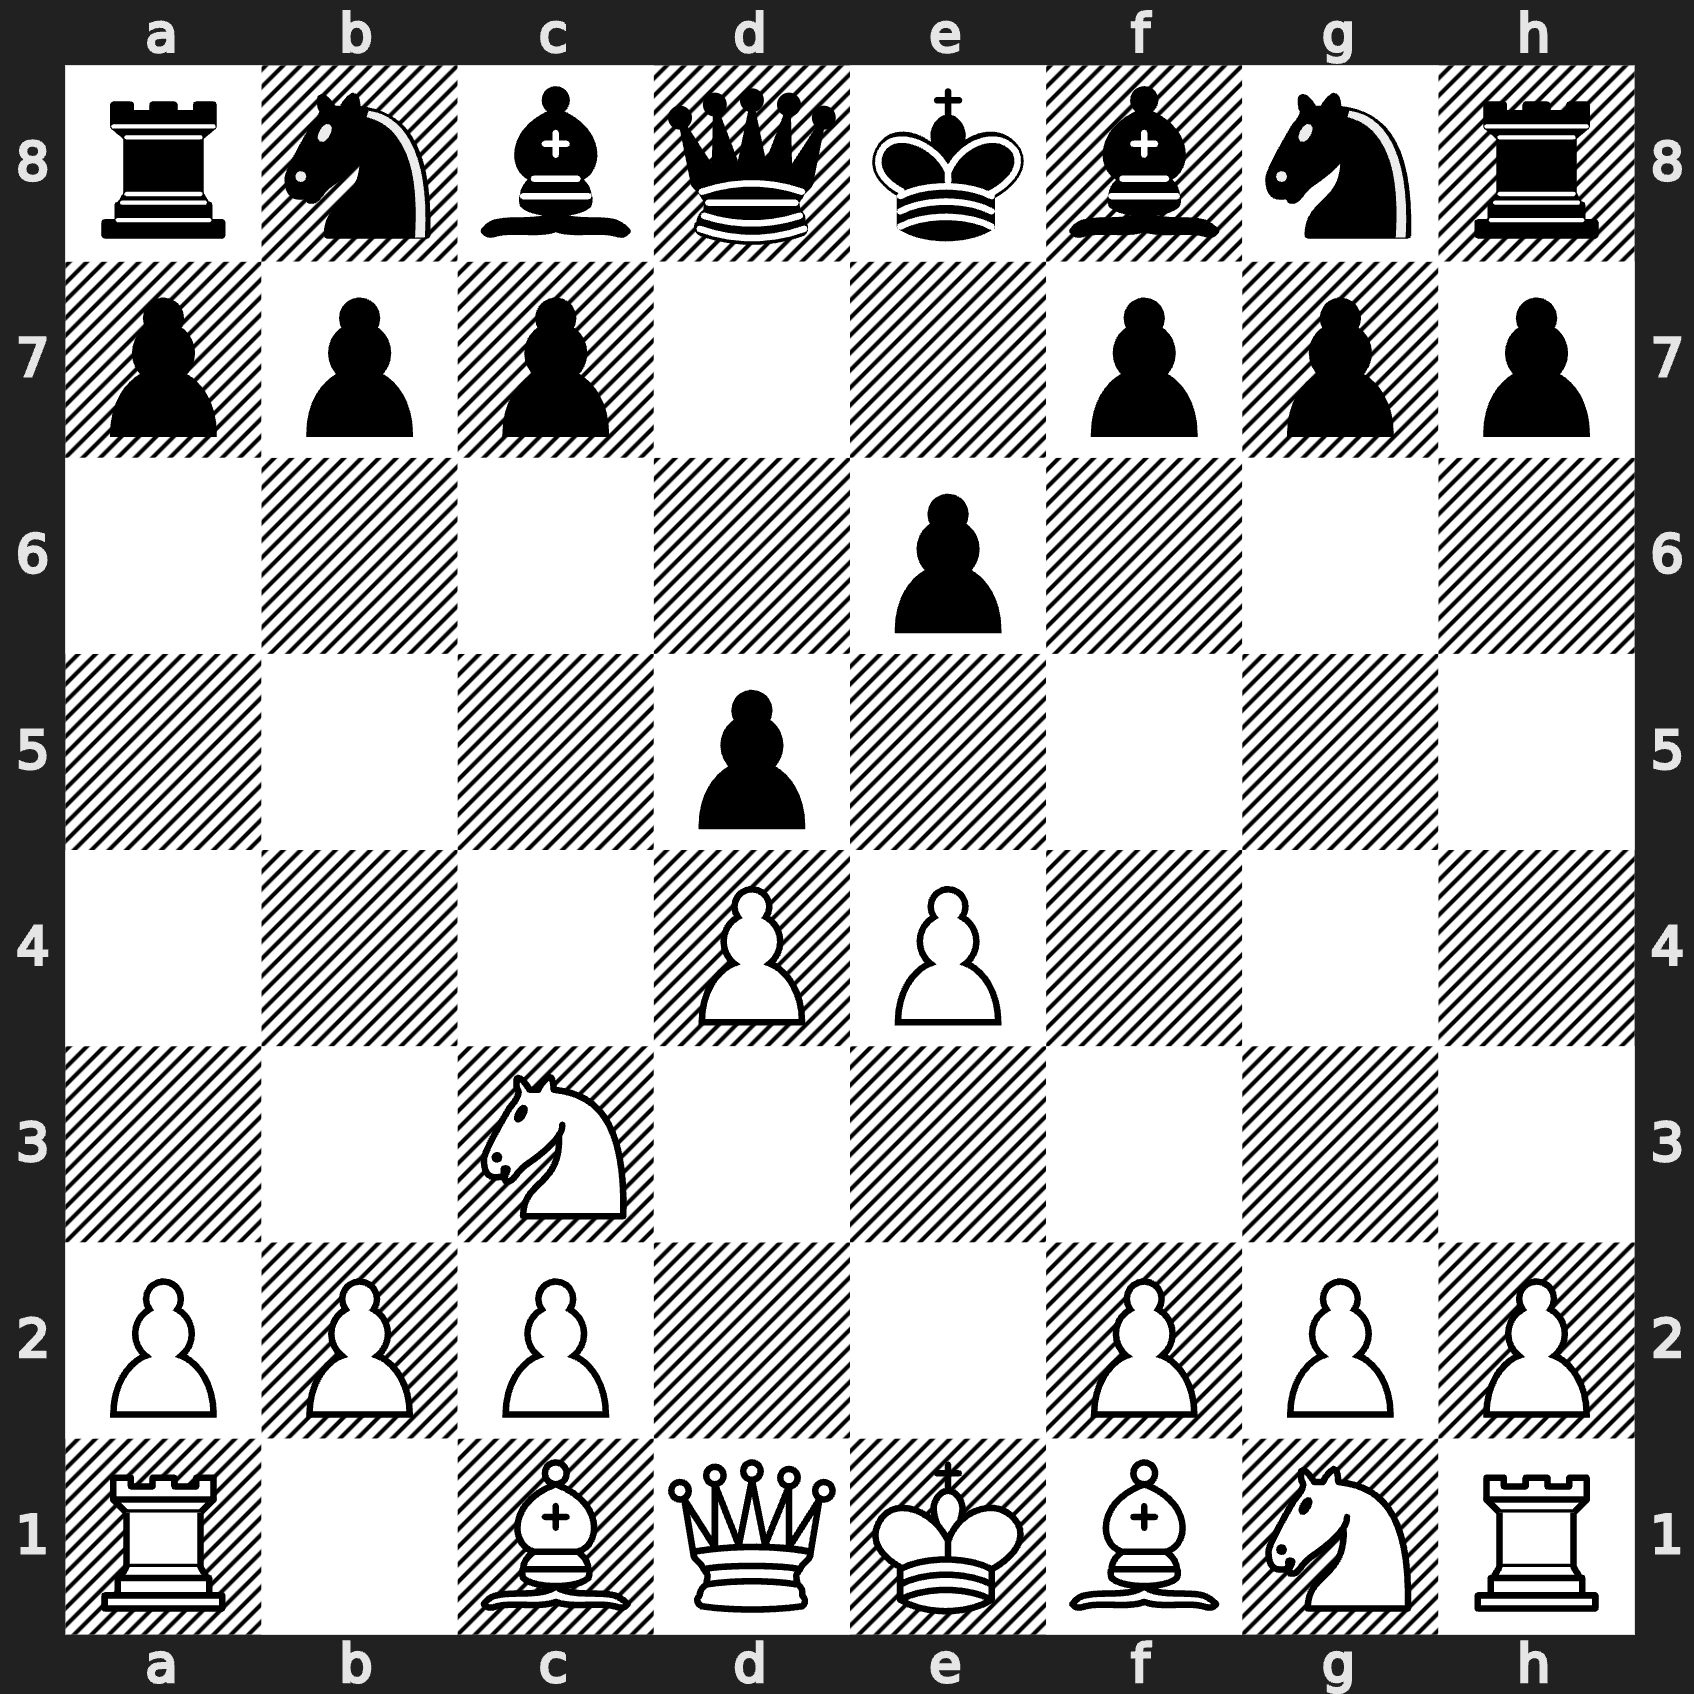
\includegraphics[width=\textwidth]{3.png}
   
    \end{minipage}\\[10pt]
  }
]
FEN: \textbf{rnbqkbnr/ppp2ppp/4p3/3p4/3PP3/2N5/PPP2PPP/R1BQKBNR b KQkq - 1 3}
\tcbline
\textbf{Human} \\
You have to simulate the following game: \\
Lichess Player (1713) vs Lichess Player (1668)\\
Time Control: 300+3\\
Time left: 5:04(Black) vs 5:02(White)\\
The last 2 moves were d7d5 b1c3 \texttt{<state>}\\
It is White's turn. Analyze the position and predict what would be the next 8 moves and the time taken for each of them? Provide your response in this format: (time taken) move1, (time taken) move2, (time taken) move3.

\tcbline
\textbf{LLAMIA} \\
Moves: (1) g8f6, (0) c1g5, (2) f8e7, (0) e4e5, (1) f6d7, (4) g5e3, (2) c7c5, (2) g1f3

\tcbline
\textbf{Human} \\
Time left: 4:55(White) vs 5:07(Black)\\
The last 1 moves were b8c6 \texttt{<state>}\\
It is Black's turn. Evaluate the position and predict what would be the next 10 moves and the time taken for each of them?

\tcbline
\textbf{LLAMIA} \\
Evaluation: -0.81\\
Moves: (1) f1b5, (1) e8g8, (4) b5c6, (0) b7c6, (2) e1g1, (0) c5d4, (28) d1d4, (1) c6c5, (14) d4g4, (8) f7f5

\tcbline
\textbf{Human} \\
Time left: 3:58(White) vs 4:33(Black)\\
The last 3 moves were d5d4\\
f3g5\\
e7g5 \texttt{<state>}\\
It is Black's turn. Evaluate the position and predict what would be the next 4 moves and the time taken for each of them?

\tcbline
\textbf{LLAMIA} \\
Evaluation: -2.09\\
Moves: (2) e3g5, (20) d8c7, (12) g5e7, (12) f8f7
\label{listing:lichess_instruction_format}
\end{tcolorbox}


\begin{tcolorbox}[
  colback=white,
  colframe=black!75!white,
  colbacktitle=black!75!white,
  title=Elite games instruction,
  enhanced,
  before upper={% Insert the figure at the top-left
    \begin{minipage}{0.3\textwidth} % Adjust width as needed
      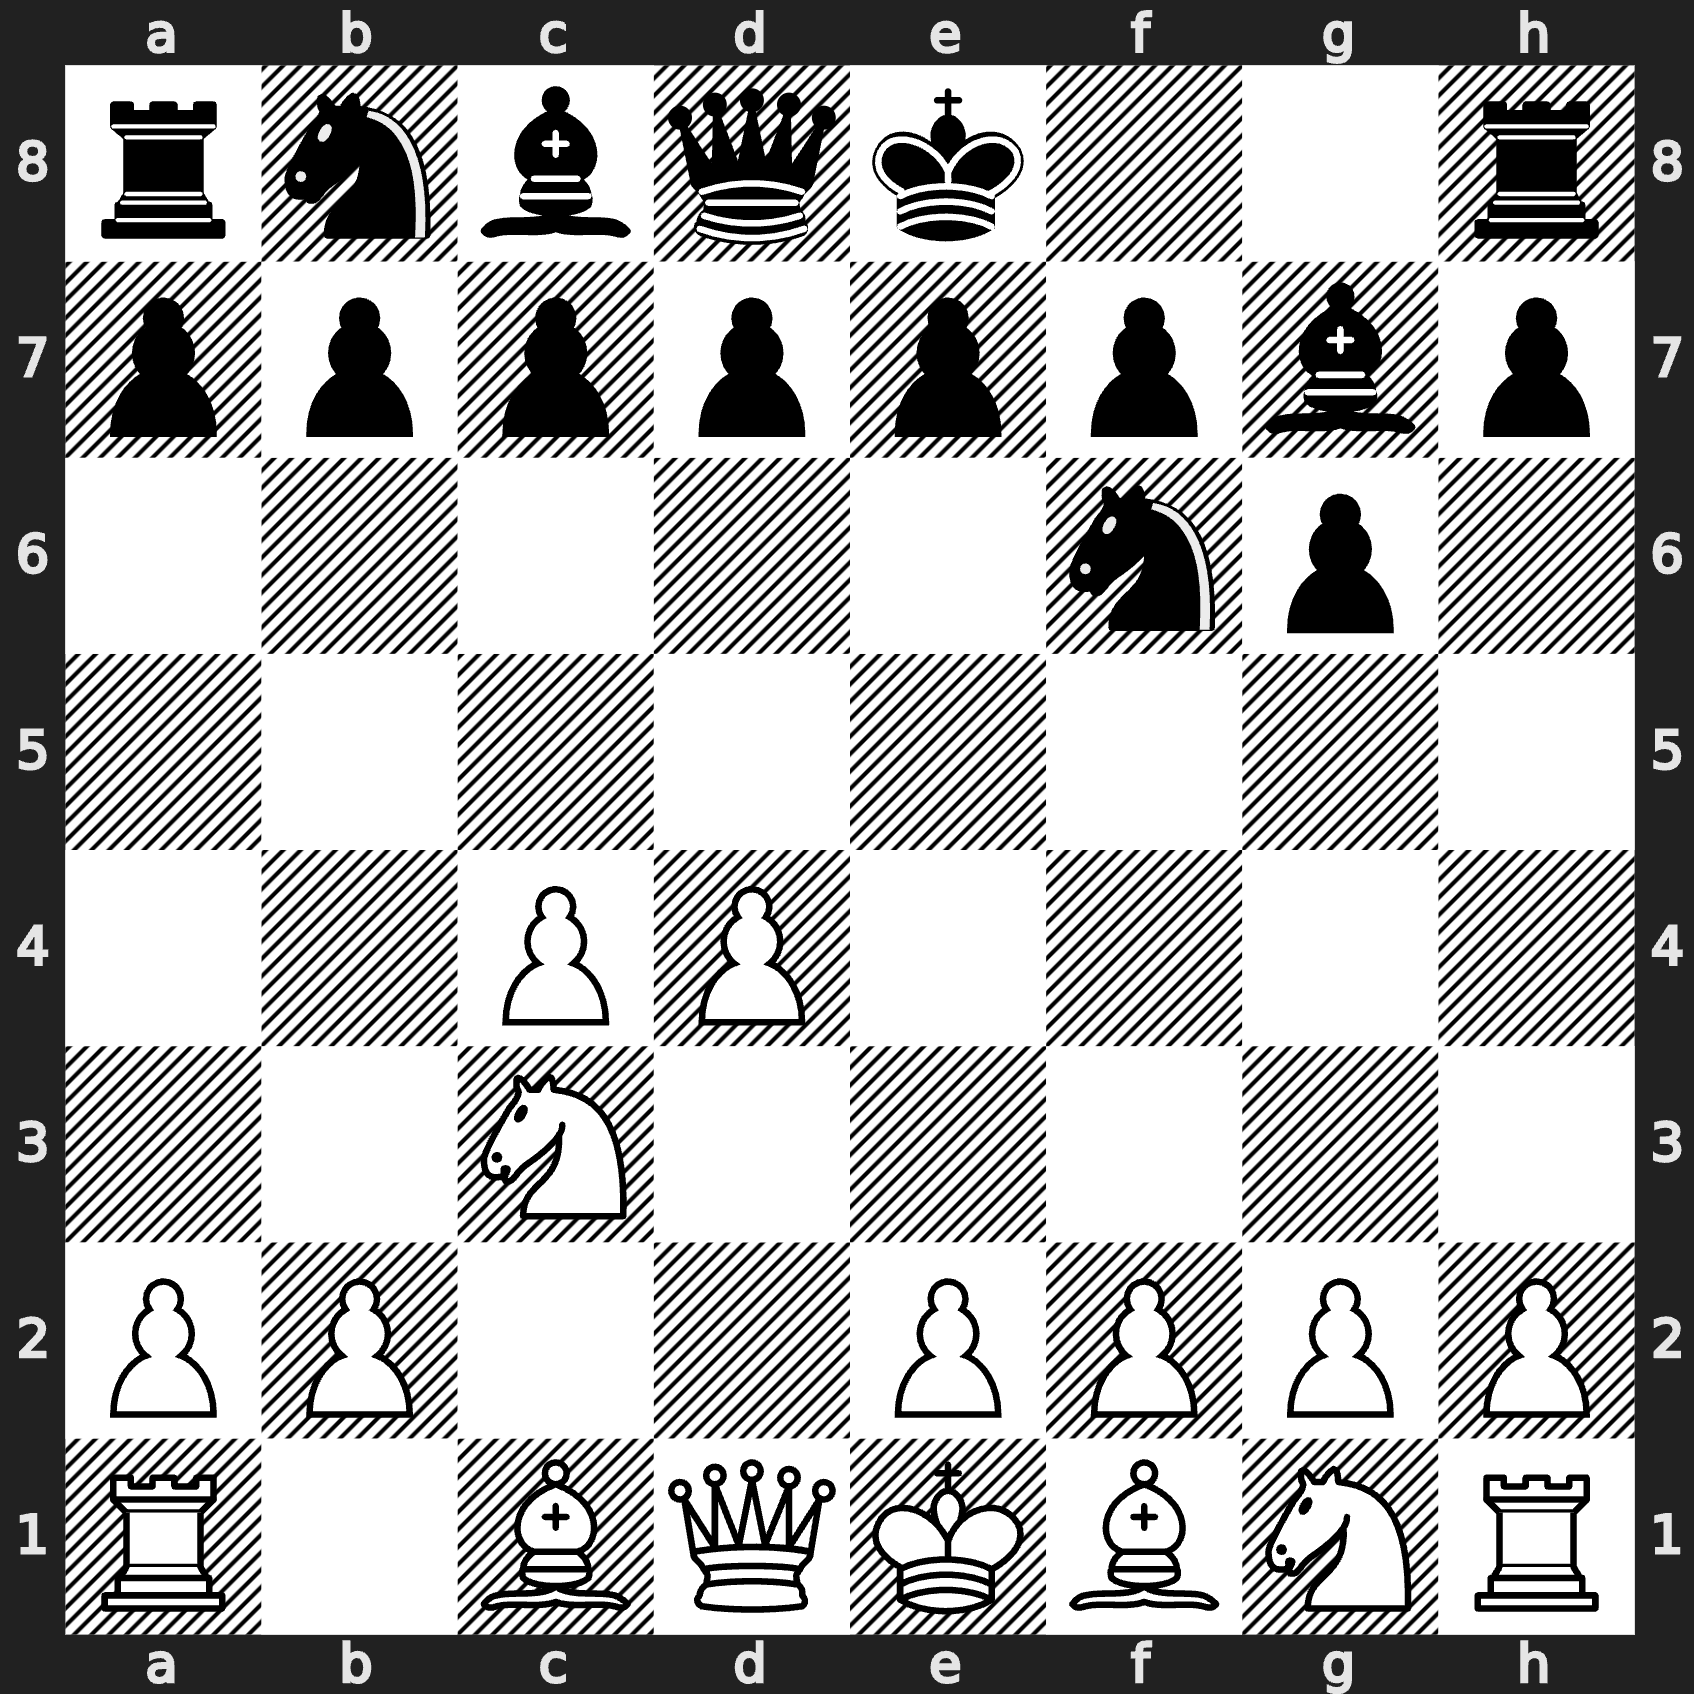
\includegraphics[width=\textwidth]{4.png}
  
    \end{minipage}\\[10pt]
  }
]
FEN: \textbf{rnbqk2r/ppppppbp/5np1/8/2PP4/2N5/PP2PPPP/R1BQKBNR w KQkq - 2 4}
\tcbline
\textbf{Human} \\
You have to simulate the following game: \\
Wang, Hao (2680) - Fedorov, Alexei (2563)\\
Rating Difference = 117\\
Event: TCh-ROU Superliga 2016\\
ECO: E83\\
Opening: King's Indian Defense, Saemisch Variation, Panno Formation\\
The last 2 moves were g7g6 b1c3 \texttt{<state>}\\
Analyze the position and predict what would be the next 3 moves. Provide your response as a list of UCI moves.

\tcbline
\textbf{LLAMIA} \\
The next moves are: f8g7 e2e4 d7d6

\tcbline
\textbf{Human} \\
The last move was d1d2 \texttt{<state>}\\
Analyze the position and predict what would be the next 10 moves.

\tcbline
\textbf{LLAMIA} \\
The next moves are: a8b8 h2h4 h7h5 e2c1 a6a5 f1e2 c8d7 e2d1 b7b6 c1e2

\tcbline
\textbf{Human} \\
Predict the winner of the game and in how many moves will the game end.

\tcbline
\textbf{LLAMIA} \\
Draw in 41 moves.
\label{listing:elite_instruction_format}
\end{tcolorbox}

\subsection{Commentary}
\begin{tcolorbox}[
  colback=white,
  colframe=black!75!white,
  colbacktitle=black!75!white,
  title=State annotation instruction,
  enhanced,
  before upper={% Insert the figure at the top-left

    \begin{minipage}{0.3\textwidth} 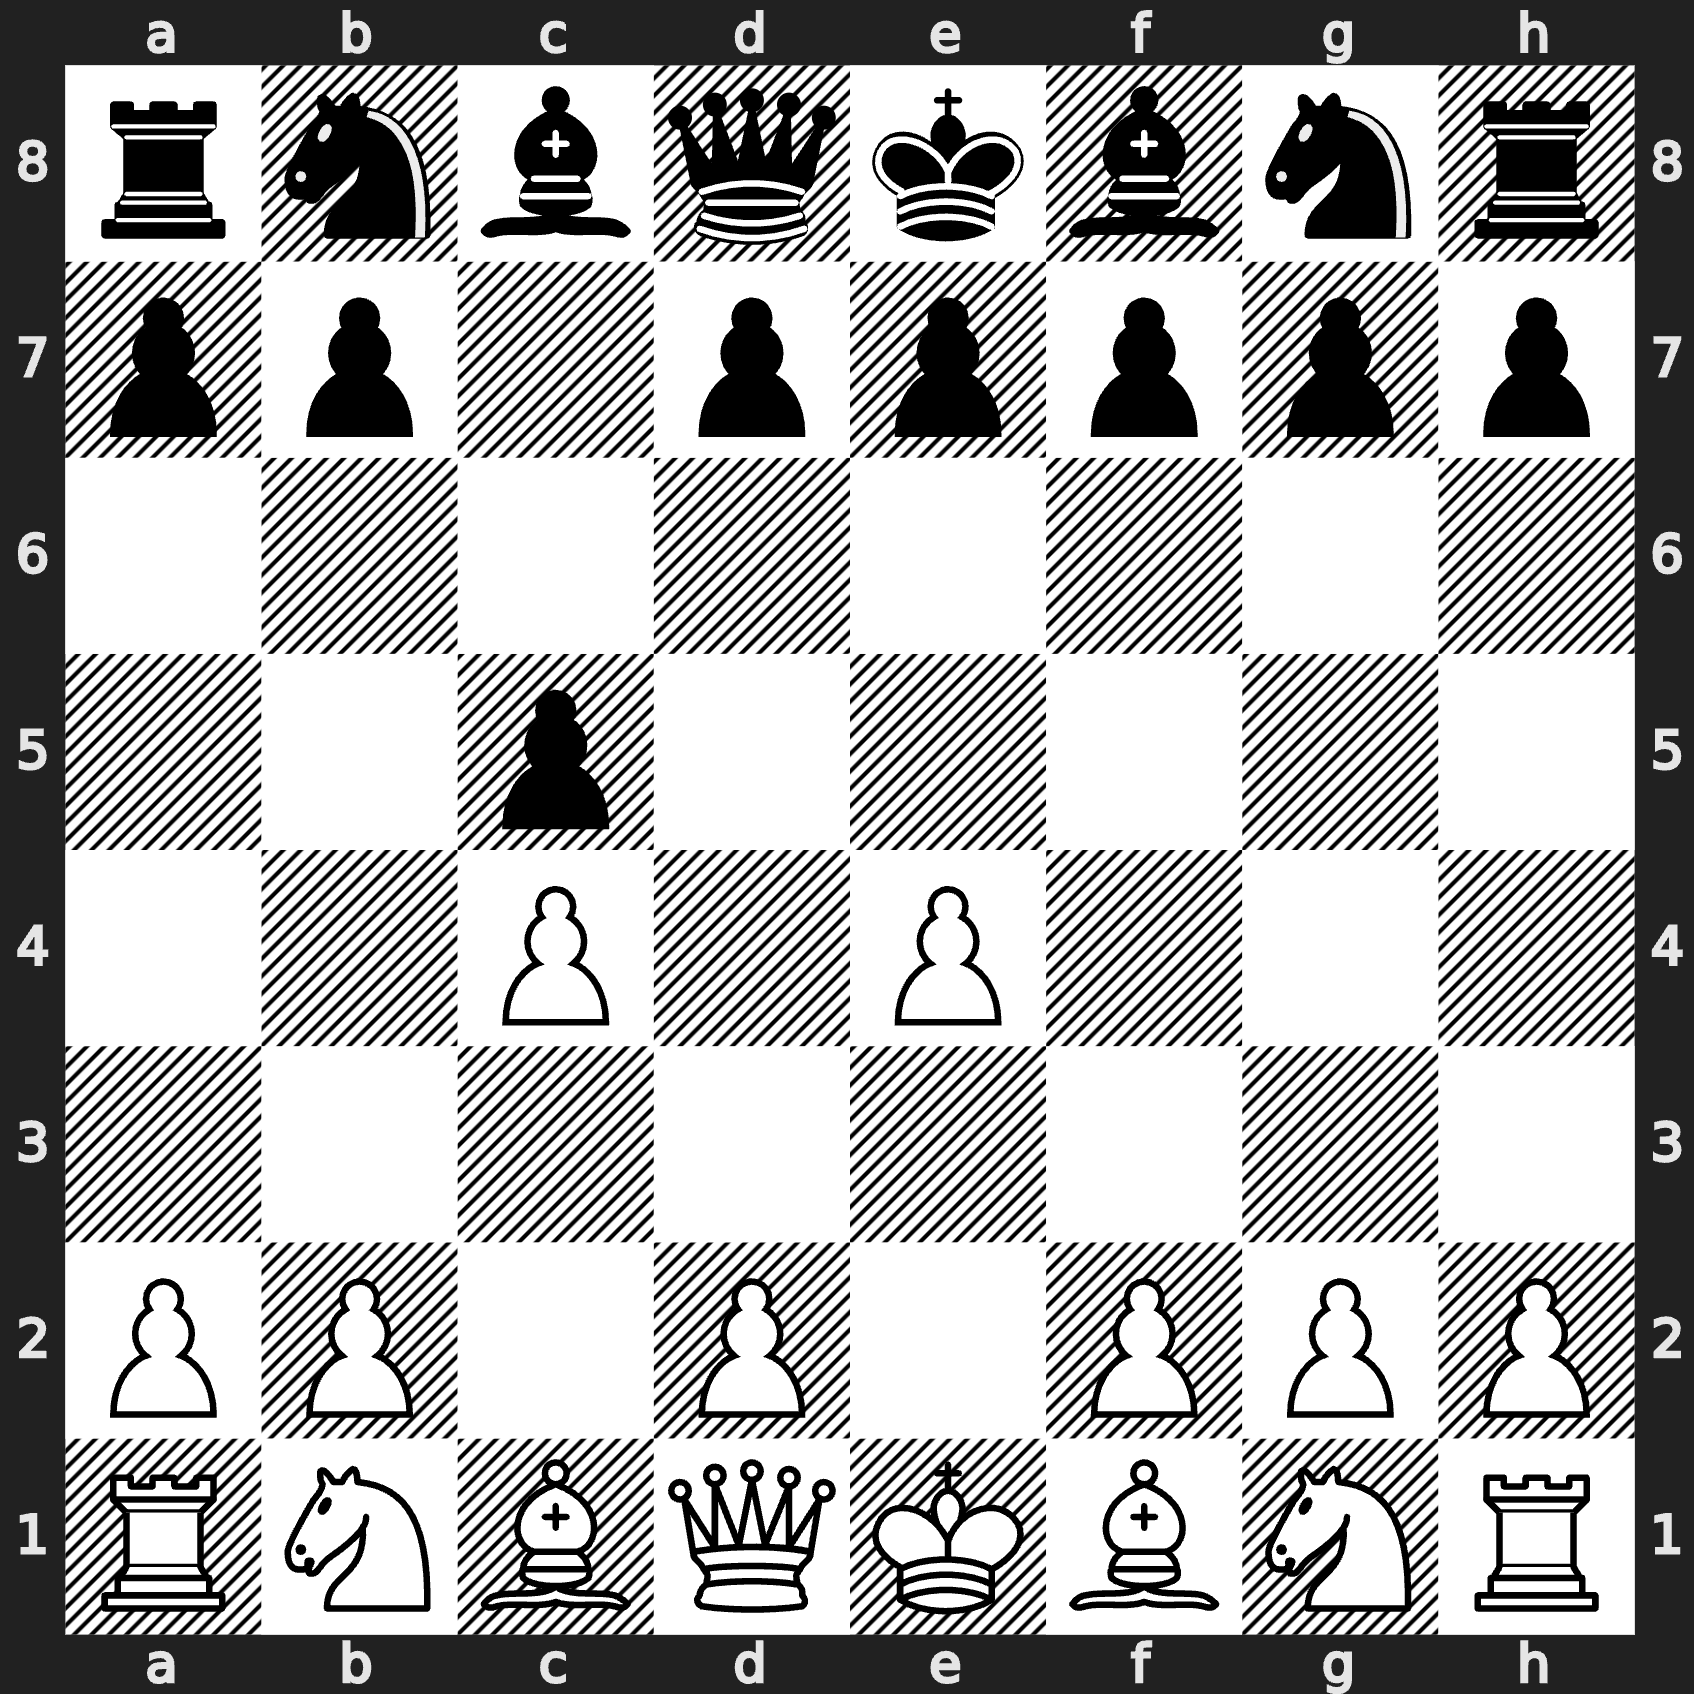
\includegraphics[width=\textwidth]{5.png}
      
    \end{minipage}\\[10pt]
  }
]

FEN: \textbf{rnbqkbnr/pp1ppppp/8/2p5/2P1P3/8/PP1P1PPP/RNBQKBNR b KQkq - 0 2}
\tcbline
\textbf{Human} \\
You have to annotate the following game: \\
OstapSuleimanBender (1784) - galeru (1704)\\
Rating Difference = 80\\
Event: Rated Rapid game\\
ECO: B20\\
Opening: Sicilian Defense: Staunton-Cochrane Variation\\
Time Control: 900+10\\
Game: 1. e4 c5 2. c4 Nc6 3. Nc3 Nf6 4. Nf3 e5 5. d3 Be7 6. a3 Nd4 7. b4 cxb4 8. axb4 Bxb4 9. Bd2 Nxf3+ 10. Qxf3 Be7 11. Qg3 d6 12. Qxg7 Rg8 13. Qh6 Rg6 14. Qh4 h6 15. Be2 Nd5 16. Qh5 Nxc3 17. Bxc3 Kf8 18. h3 Kg7 19. Bd2 Rxg2 20. Bxh6+ Kg8 21. Bg4 Bh4 22. Rf1 Qf6 23. Be3 Bxg4 24. hxg4 Kg7 25. Qf5 a6 26. Rb1 b5 27. cxb5 axb5 28. Rxb5 Qxf5 29. gxf5 Ra1+ 30. Ke2 Ra2+ 31. Kf3 Rh2 32. Rd5 Kf6 33. Rxd6+ Ke7 34. Rd5 Kf6 35. Rb5 Bg5 36. Bxg5+ Kxg5 37. Rxe5 Rh3+ 38. Kg2 Kg4 39. d4 Rg3+ 40. Kh2 Rf3 41. Kg2 Kf4 42. Re7 Rg3+ 43. Kh1 Rd3 44. d5 Kf3 45. Kg1 Rdd2 46. f6 Rxf2 47. Rxf2+ Rxf2 48. d6 Rg2+ 49. Kf1 Rd2 50. d7 Rd1\# \\ 

Annotate the move: 2. c4 \texttt{<state>}

\tcbline
\textbf{LLAMIA} \\
B20 Sicilian Defense: Staunton-Cochrane Variation

\tcbline
\textbf{Human} \\
Annotate the move: 3. Nc6 \texttt{<state>}

\tcbline
\textbf{LLAMIA} \\
Feels like e6 or Nf6 would be more principled, but the d4 square is kind of nice?
\label{listing:state_annotation_format}
\end{tcolorbox}

\begin{tcolorbox}[
  colback=white,
  colframe=black!75!white,
  colbacktitle=black!75!white,
  title=Commentary instruction,
  enhanced,
  before upper={% Insert the figure at the top-left
    \begin{minipage}{0.3\textwidth} % Adjust width as needed
      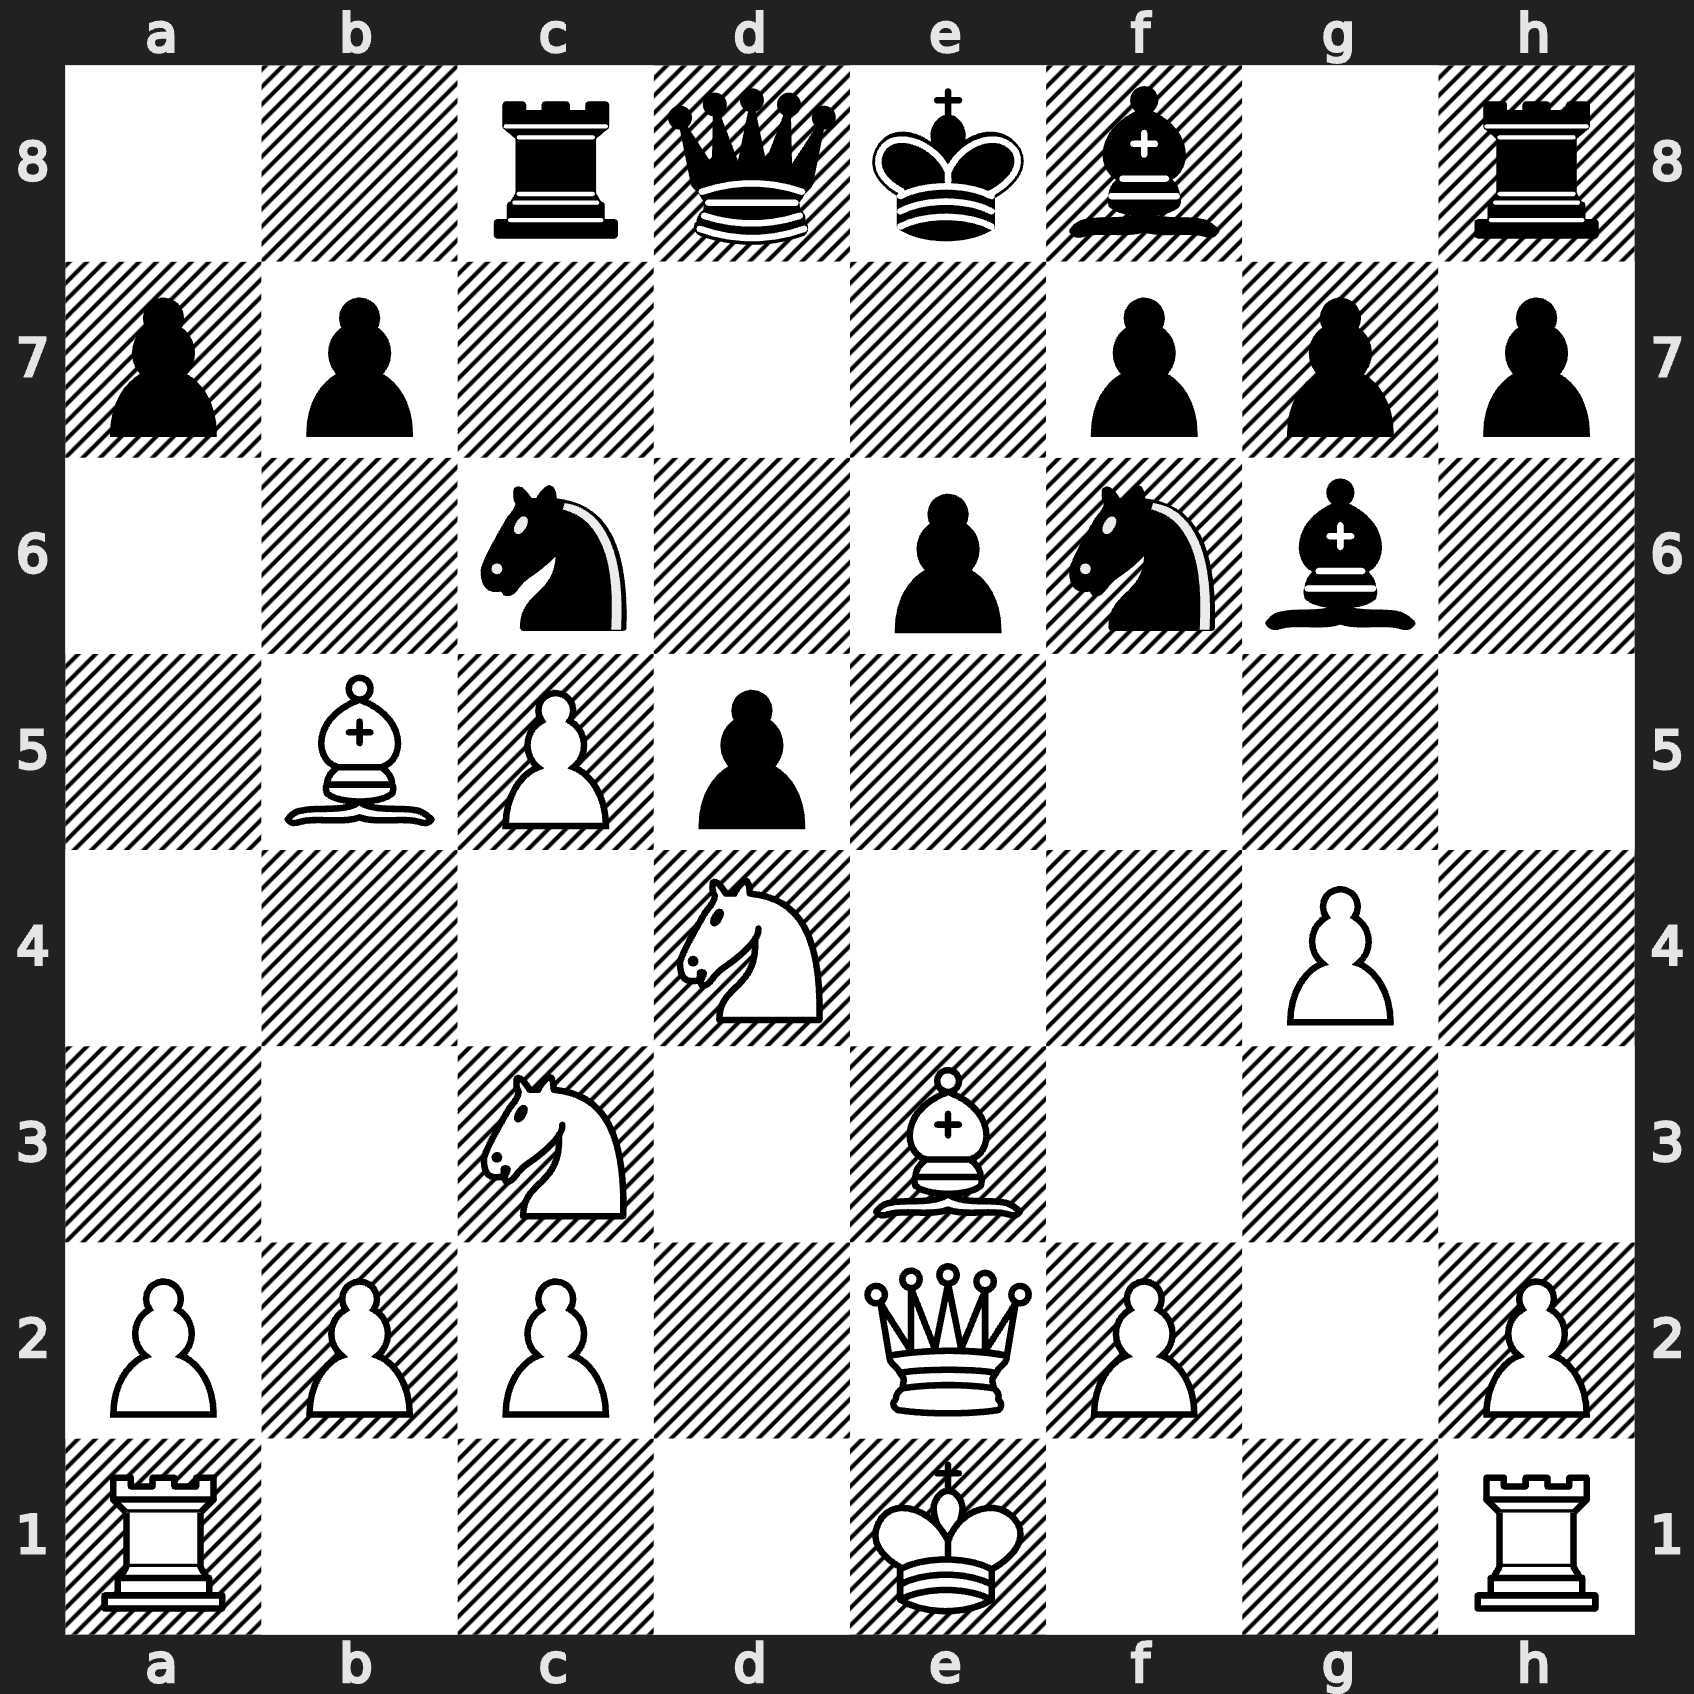
\includegraphics[width=1.0\textwidth]{6.png}
      
    \end{minipage}\\[10pt]
  }
]
FEN: \textbf{2rqkb1r/pp3ppp/2n1pnb1/1BPp4/3N2P1/2N1B3/PPP1QP1P/R3K2R w KQk - 6 12}\\
\tcbline
\textbf{Human} \\
You have to generate commentary for the following game: \\
Geoff Chandler vs Richard Kynoch \\
1.\ e4 c6 2.\ d4 d5 3.\ e5 Bf5 4.\ Nc3 e6 5.\ g4 Bg6 6.\ Nge2 c5 7.\ Be3 Nc6 8.\ dxc5 Nxe5 9.\ Nd4 Rc8 10.\ Bb5+ Nc6 11.\ Qe2 Nf6 12.\ O-O-O Be7 13.\ h4 h5 14.\ f3 Nd7 15.\ gxh5 Rxh5 16.\ Rhg1 Nxd5 17.\ Bxd4 Qc7 18.\ Rxg6 fxg6 19.\ Qxe6 Rf5 20.\ Nxd5 Qd8 21.\ Qxg6+ Rf7 22.\ Re1 Kf8 23.\ Qh7 Ke8 24.\ Qg8+ Rf8 25.\ Qxg7 Rf7 26.\ Qg8+ Rf8 27.\ Nf6\#. \\

You will be provided with segments of moves from this game, one after the other, and your task is to commentate on the segment.\\[3pt]
\texttt{<state>}
\textbf{Moves:} 12.\ O-O-O Be7 13.\ h4 h5 14.\ f3 Nd7 15.\ gxh5 Rxh5 
\tcbline
\textbf{LLAMIA} \\
We have a queenside castle by Chandler [12. O-O-O] and bishop to e7. [12… Be7] h4 [13. h4]  h5 [13… h5] f3 [14. f3], knight to d7 [14… Nd7] and g captures on h5 [15. gxh5] and this is definitely the critical position of the game. If black continued this game with (15… Bxh5) Bishop captures on h5 everything would be perfectly okay, and well black would continue this game being better. But Mr. Kenock decided to play rook captures on h5 [15… Rxh5] and this is where his troubles begin.
\label{listing:commentary_format}
\end{tcolorbox}


\section{Hyperparamaters}
\label{sec:hyperparams}
LLAMIA models (7B, 13B) were trained on five nodes of 80GB A100 GPUs, totaling
approximately eight days of computational budget.


\begin{enumerate}
  \item \textbf{Model Architecture}
  \begin{itemize}
    \item Backbone LLM: \texttt{lmsys/vicuna-13b-v1.5}
    \item Agent Model: \texttt{Lc0-BT4}
    \item Hidden size (LLM): 5120
    \item Agent encoder dimension: 1024
    \item Number of agent encoders: 15
    \item Number of LLM state tokens: 16
    \item Number of agent state tokens: 64
    \item Projector type: \texttt{SimpleMLP}
    \item Projector hidden dimension: 2048
    \item Projector hidden depth: 3
    \item Projector dropout: 0.1
    \item Projection layer: \texttt{encoder[\textbackslash d]+/ln2}
    \item Use state patch token: \texttt{true}
    \item Freeze LLM backbone: \texttt{true}
  \end{itemize}

  \item \textbf{Training Configuration}
  \begin{itemize}
    \item Number of epochs: 1
    \item Per-device train batch size: 70
    \item Per-device eval batch size: 32
    \item Learning rate: 6e-5
    \item Optimizer: AdamW (\(\beta_1 = 0.9, \beta_2 = 0.999, \epsilon = 10^{-8}\))
    \item Max gradient norm: 1
    \item Scheduler: Cosine
    \item Warmup ratio: 0.05
    \item Gradient accumulation steps: 1
    \item Gradient checkpointing: \texttt{true}
    \item Mixed precision: bfloat16 
    \item Quantization: \texttt{nf4}
    \item Double quantization: \texttt{true}
    \item Deepspeed config: Deepspeed Zero2 with Offload
  \end{itemize}

\end{enumerate}


\section{Paper rewrite items}
Neurips
\begin{itemize}
    \item variables unclear in eqn1
    \item 
    
    
\end{itemize}


\end{document}


% This document was modified from the file originally made available by
% Pat Langley and Andrea Danyluk for ICML-2K. This version was created
% by Iain Murray in 2018, and modified by Alexandre Bouchard in
% 2019 and 2021 and by Csaba Szepesvari, Gang Niu and Sivan Sabato in 2022.
% Modified again in 2023 and 2024 by Sivan Sabato and Jonathan Scarlett.
% Previous contributors include Dan Roy, Lise Getoor and Tobias
% Scheffer, which was slightly modified from the 2010 version by
% Thorsten Joachims & Johannes Fuernkranz, slightly modified from the
% 2009 version by Kiri Wagstaff and Sam Roweis's 2008 version, which is
% slightly modified from Prasad Tadepalli's 2007 version which is a
% lightly changed version of the previous year's version by Andrew
% Moore, which was in turn edited from those of Kristian Kersting and
% Codrina Lauth. Alex Smola contributed to the algorithmic style files.
\begin{comment}
    \section{Feedback}
Continous vs Discrete

\begin{enumerate}
    \item What defines a foundational model?
    \begin{enumerate}
        \item (Bommasani et al. 2021). Foundation models constitute large-scale AI models that are pre-trained on vast amounts of general data and that can be adapted for downstream applications (e.g., by fine-tuning them through further training on application-specific data). Through this pre-train and adapt approach they expedite the development of innovative AI products and services and accelerate the accessibility of high-performance AI solutions in various industries (Teubner et al. 2023).
        \item With scaling, foundation models are becoming increasingly good at performing tasks they were not explicitly trained for, thereby broadening the scope of applications achievable by a single model without the need for additional training data or fine-tuning (Brown et al. 2020).When needed, task-specific performance can be further enhanced through fine-tuning or effective prompt engineering techniques; (Liu et al. 2023; Niu et al. 2020).
        \item Following Bommasani et al. (2021, p. 1), we define a foundation model as ``any model that is trained on broad data that can be adapted to a wide range of downstream tasks''. Through this combination of task-agnostic pre-training and subsequent fine-tuning, foundation models enable new approaches to building and deploying AI systems.
        \item Emergent Capabilities The first key feature of foundation models is the emergence of behavioral capabilities that were not explicitly constructed, nor expected, by human developers, which frequently is referred to as in-context learning (Min et al. 2022)
        \item \cite{XXXFlava} a true foundation model in the vision and language space should not only be good at vision, or language, or vision-and language problems–it should be good at all three, at the same time.
    \end{enumerate}
    \item What would characterize a foundational decision model
    \item What constitutes an FDM
    \item Why Chess
    \somesh{P2 @Harini ChessFormer, AlphaZero}
    \begin{itemize}
        \item 
    \end{itemize}
    \item Emergent Properties across Large Decision Models
    \item Why search or runtime compute
    \item Why Language and Decisions
    
\end{enumerate}








Planning is a key task in real-world scenarios whiuch has not been solved in the generality needed by any foundation models [cite: Yann Le Cun tweeted a reference for this]. 

Foundation models for decision making should look like... creation of adapters - one per environment. We provide one approach - RLQA to create foundation models for decision making.

Task specific specialist models have their own disadvantages such as limited generalizability. To get the best of these two approaches, researchers have proposed coupling LLMs with specialist policies using toolformers, agentic models etc. [cite: ].



However, this loose coupling cannot solve tasks which require the LLM to understand the specialist policy. Some concrete examples of such tasks include commentary generation in games, language conditioned policy adaptation, language based behavior generalization etc. To bridge this gap, we propose an approach called RLQA, where we tightly couple the LLM and the specialist policy using a policy-language adapter. In this paper, we present an approach to train this adapter, provide benchmarks to test the efficacy of the coupled LLM and specialist policy and provide demonstrations of tasks where our RLQA approach significantly outperforms other popular approaches in literature either in terms of accuracy or efficiency. In this paper, we restrict attention to chess, but our approach is extensible to any planning problem in general.

Fig-1 with descriptive caption - inference pipeline
One paragraph on approach and motivation, novel tasks, datasets and benchmarks


Generalist agent for a single environment - can generate/simulate multiple behaviors in a text controlled manner. A method to align an agent and an LLM a foundation model in decision making and decision understanding
Emergent properties on unseen tasks
Bridging the gap between specialized agents and LLMs via our own connectors:
1. to solve greater tasks which cannot be solved by these independently or weakly coupled
2. example commentary generation, fine-tuned behavior cloning, conditional decision making - example opponent/environment conditioning


Contributions need to be differentiated - Benchmark vs Algorithm vs Model \somesh{1 Algorithm, 3 Datasets, 4 Benchmarks How should we do this?}

Benchmark: Are we providing an arena for testing other RL agents? \somesh{Yes}


Effectiveness of Generalized Decision Making - needs to be defined... \somesh{Conditional Decision Making - Similar to Behavior, Explanation - Directly state annotation, game analysis. Agent identification- Cheating Detection, Improving search - LLMCTS :P}

\begin{enumerate}
    \item What is a foundational model ? A foundation model is any
model that is trained on broad data (generally using self-supervision at scale) that can be adapted (e.g., fine-tuned) to a wide range of downstream tasks; current examples include BERT [Devlin et al.2019], GPT-3 [Brown et al. 2020], and CLIP [Radford et al. 2021]
\end{enumerate}

\somesh{What to capture: What does a foundational decision making model need, an LLM and a policy or representation learning model, and a generalized method to connect these. What should it be trained on? Large Unsupervised number of decisions, and rewards/evaluation.}
\subsection{Contribution}
1. Foundation Decision models
    1.1 Behaviour cloning in few shots, or IFT with 10\% of the data, one model vs finetunes.  Table 1
    1.2 Behaviour stylometry: Unseen task, Comparable or better results with, 15\% of  shots across 20,40,112,High Ranked, GMs, Bots, Elo identification, Time formats table 1.3 
2. We are able to get the strongest known raw policy 
https://arxiv.org/pdf/2402.04494

2. Comparison against Llama3.1 405B with tool calling to Lc0 + MCTS, and GPT-4o with Evaluation and next best moves from Lc0 + MCTS. (All tables) Projection tokens in FDM perform better than tool calling on more than 30x larger LLMs. (All tables)

3. What can an FDM do? Results breakdown why are FDMs needed
    1. Only LLM tasks: position description
    2. Only Engine tasks: puzzle
    4. One model to all
    3. Neither finetune nor agentic task: commentary, position difficulty, rating,
Breadth of tasks with the star-graph

4. What data goes into an FDM:
    1. Self-supervised large scale data (Existing positions and their evals)
    2. Demonstrations from humans (BC)
    3. Complex Instruction data (small scale, downstream applications)

5. Results and analysis
Appendix Lucena

6. Extend this to other envs.


OPenreview
1. Towards building a foundation decision model



4. Commentary generation, 

5. Decision Understanding
https://aclanthology.org/P18-1154.pdf
https://aclanthology.org/P19-1597.pdf
https://arxiv.org/pdf/2212.08195
5. Emergent Abilities unlocked via jointly training with agent projections: Breadth of tasks
6. Towards fdm ?

1. Using Decisions or Policy as a modality unlocks downstream capabilities. (LLaVA sense - DT is an input as opposed to a competition)
    Relevant Results:
        a. State Value Multi Choice, Annotation, Commentary, BOT classification, Puzzles Understanding, Game Masking
        b. Downstream capabilities such as game or
state commentary generation, we outperform SOTA models and even upto 10x larger LLMs
assisted with super-human engines

2. LLMs with Optimal Policy are effecient 0-shot behavior cloners (simulators)
    a. Behavior cloning all results

3. LLMs are strong and efficient look ahead models
    3.1 LLMs themselves model N-step lookahead better than agent trained on that task (Performance, Data required)
    3.2 LLMs that learn look ahead modelling improve downstream performance (tasks)

4. 
\section{Learning to Look Ahead}
Any problem that requires planning can be described by

\begin{enumerate}
    \item A problem statement or current state (S)
    \item A proposed solution or Action (A)
    \item Approximate feedback (F)
    \item An agent or policy (P) that can generate sub-optimal or near-optimal actions.
\end{enumerate}
Current research solves this task by using (P) obtained from self-supervised learning on large amounts of data, as a heuristic to do a "search", or a chain of intermediate actions, which progressively lead to $max(F)$. The resulting search, the tree of actions, is able to solve the problem statement better.

In this work we try to answer the following questions

\begin{enumerate}
    \item Can LLMs exploit an agent's heuristic to plan N-step ahead? We know that Lc0's NN has a policy of only 2600, + MCTS 3500
    \somesh{Note to self: For general problems the LLM itself is the agent}
    \begin{enumerate}
        \item We further train the agent to predict the optimal actions -> +21
        \item We train RLQA to predict the optimal actions -> +53
        \item We train RLQA to predict the optimal actions and the chain-of-thought (the best path in the tree of actions) to it -> +143
    \end{enumerate}

    \item What is the value of the explicit search (
\end{enumerate}
1. Can LLMs exploit an agent's heuristic to plan N-step ahead?
    1.1. We train an agent to predict the optimal policy -> +21
    1.2. We train Agent+LLM to predict the optimal policy -> +53
    1.3. (Train-time) We train Agent+LLM to predict the ToT + optimal policy -> +143 -> Input: FEN(Board) -> Output: Evaluation and next best moves until 30 depth (3500 Elo)
    1.4. (Train-time) We train Agent+LLM to predict the ToT + optimal policy -> +143 -> 
        Input: FEN(Board)
        Output: Evaluation + (next best moves + environment verbalization) until 30 depth (3500 Elo)
        Ablations 1. Only ground truth 2. Synthetic w Ground truth (Agadmator vs Crowd sourced vs Random Tokens)
    1.5. (Train-time) We train Agent+LLM to predict the ToT + optimal policy -> +143 -> 
        Input: FEN(Board)
        Output: Evaluation + (next best moves + annotation/commentary) until 30 depth (3500 Elo)
    1.6. (Train-time) We train Agent+LLM to predict the ToT + optimal policy -> +143 -> 
        Input: FEN(Board)
        Output: Evaluation + (next best moves) until 30 depth (3500 Elo) + Commentary/Annotation of the 3500 Elo
    1.7. (Game-level commentary) We train Agent+LLM to predict the ToT + optimal policy -> +143 -> 
        Input: FEN(Board)
        Output: Evaluation + (next best moves) until 30 depth (3500 Elo) + Commentary of the 3500 Elo
    
2. What is the value of the explicit search tokens?
    2.1. We train an agent to predict the (ToT + optimal policy), Infer w/o ToT -> +76

3. How can we train an LLM to plan with progressive Tree of thoughts
    3.1 We IFT the optimal path and pruning -> +36
    3.2 We IFT the optimal path and pruning progressively -> +75
        Input -> FEN
        Output -> Eval + Next-best move

O1 analogy, 


Parameter Count Trend
1. Concluding that what may not work for smaller models may not translate to stronger models

\section{Model}
\emph{Getting representations from an expert engine, adapting it and then feeding the adapted representation to an LLM to do the following downstream tasks - multi-choice chess annotation, checkmate puzzles, state-value multi-choice, encoding <--> PGN (verbalization) bidrectional; need to check if adding the encoding helps at all, \textbf{behavior simulation (ACM 2018, Maia Chess) - one model, multiple Elos (and also one specific player), accuracy, commentary generation (beating SOTA based on state-level commentary generation - we will do trajectory-level)}}

We consider the standard MDP based RL framework with the usual notation. Let $\pi^*$ denote a learnt (optimal) policy using any RL based approach that also yields $Q^*$, the optimal state-action values. We then look at the following problems:
\begin{enumerate}
    \item Policy Explanation: Given $\pi^*$, $Q^*$, the corresponding state space $\mathcal{S}$ and a state featurizer (could be a textual featurizer), we create a dataset $\widehat{\mathcal{D}}$ of $\{(S_t, f_t, A_t, Q_t,)_{t=0}^T \}_{i \in \mathcal{D}}$, where:
    \begin{enumerate}
        \item $i$ represent an episode from $\mathcal{D}$ which is an offline (can be batch or online as well) dataset of episodes/trajectories.
        \item $t \in \{0, T\}$ represents the step in the episode.
        \item $S_t \in \mathcal{S}$ represents the state at time $t$.
        \item $f_t$ represents the verbalized features of $S_t$.
        \item $A_t \sim \pi^*(S_t)$ represents the action chosen at time $t$ using policy $\pi^*$.
        \item $Q_t = Q^*(S_t, A_t)$ represents the action-value starting from state $S_t$ and choosing action $A_t$.
    \end{enumerate}
    Using this dataset, $\widehat{\mathcal{D}}$, as a first task, we finetune an LLM to predict the $Q$ values given the rest of the sequence. For the purpose of this experiment, we consider the following potential list of environments:
    \label{ref:Candidate envs for text}
    \begin{enumerate}
        \item \url{https://github.com/carla-simulator/carla}
        \item \url{https://github.com/microsoft/TextWorld}
        \item \url{https://github.com/ronentk/TextLabs}
        \item \url{https://github.com/IBM/visual-hints-textworld-rl}
        \item \url{https://github.com/google-deepmind/open_spiel}
        \item \url{https://github.com/Farama-Foundation/Minigrid}
        \item \url{https://github.com/allenai/ScienceWorld}
        \item \url{https://github.com/fidler-lab/social-driving}
        \item \url{https://github.com/google-deepmind/android_env}
        \item \url{https://github.com/facebookresearch/nocturne}
        \item \url{https://github.com/microsoft/CyberBattleSim}
    \end{enumerate}
\end{enumerate}

10M games existing
600B positions pre-existing SF-16

No. of possible positons >>> 600B positions pre-existing SF-16

Twitter:

Dataset: -> Low time
Agent -> Time series
Training -> Low time
Evaluations -> Transsuasion time



\section{Extension}
\subsection{Video Planning}
For long videos LLMs are used to generate video plans, \cite{VideoStudio,DirectorGPT} we will generate multi scene ads, we will plan it with FDM .

1. Optimal Decision making -> Ad Plan Generation from title, intent
2. Conditional Decision making -> Ad Plan generation given scene, conditions etc.
3. GDU/Commentary: Explain a scene (describe, 

1. Decision Making -> Video Plan Generation (memorable, likes/views)
2. Generalised Decision Making (Scene Fill / Complete) -> Behaviour Cloning (GDM)
3. -> Decision Understanding
\subsection{MultiGame DT}

\newpage
SFT: Transsuasion [Vicuna(13B)]: 0.31
Agent: Chronos-base (univariate): 0.09
Agent: Chronos-base (self+industry): 0.17
Pretrain: LLAMIA[Vicuna(13B) + Chronos-base (self+industry)]: 0.28
Pretrain+SFT: LLAMIA[Vicuna(13B) + Chronos-base (self+industry)]: 0.49

\somesh{Qualitative analysis of what LLM learnt from TS agent}
\somesh{Add LLM hidden state into chronos embedding}
LLM Learnt Optimal Policy:



LLAM:
    Input:
        Board position embedding + FEN 

    Output:
        (+7.2) Moves: m1 m2 m3 m4
        Also PV1: 6.1 m1, m2, m3


Finetuned Vicuna:
    Input:
        Board FEN, SV, Evaluation is (+7.2) on move m1

    Output: 
        m2 m3 m4
\begin{figure}[!h]
    \centering
    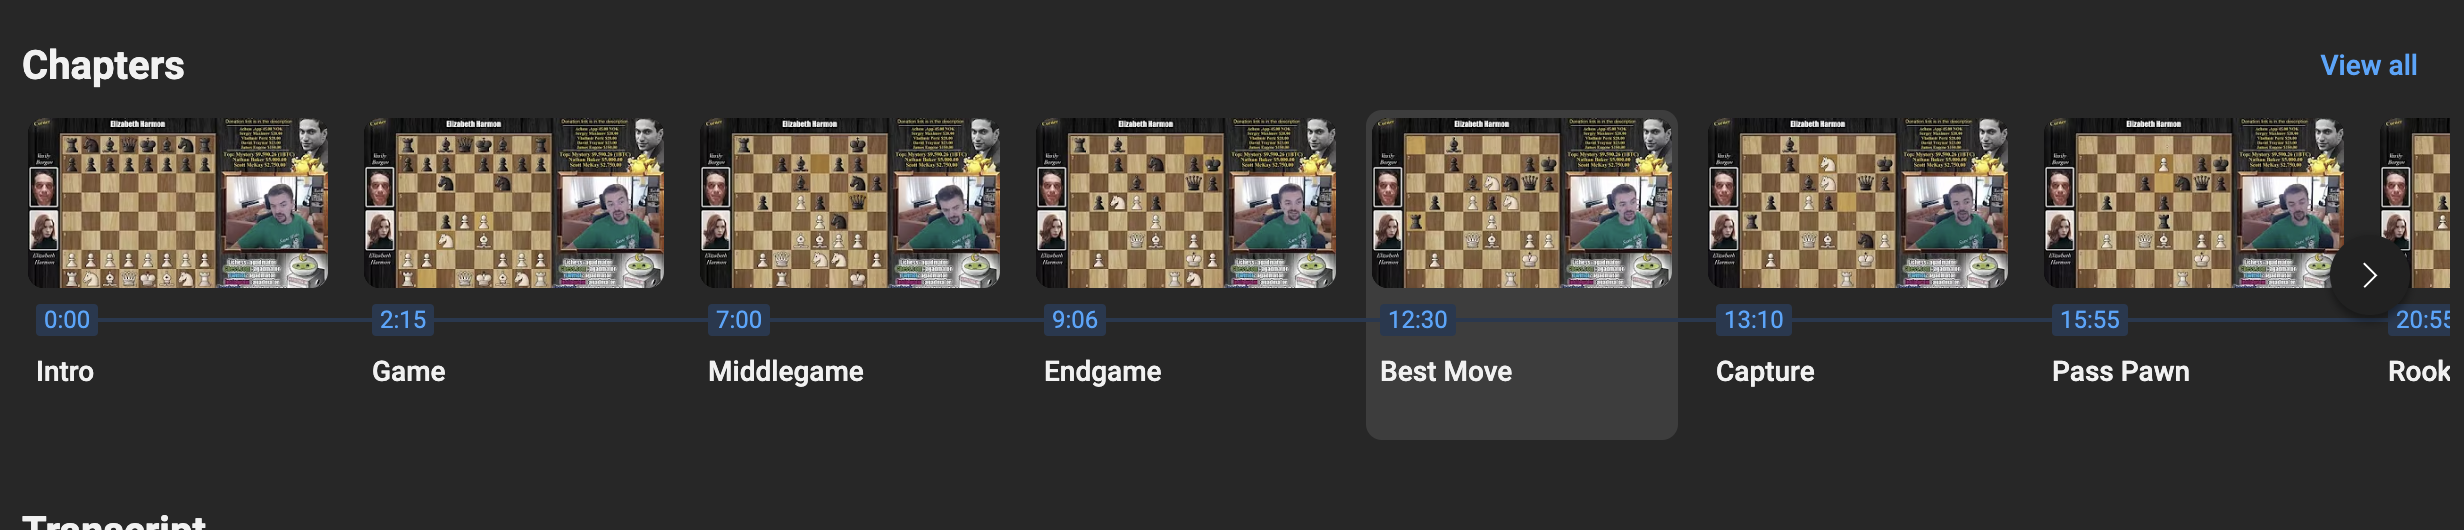
\includegraphics[width=\linewidth]{Screenshot 2025-01-22 at 5.18.04 PM.png}
    \caption{Game Commentary: Qualitative game segments annotated, with panel wise transcripts, compared with actual and GPT-4o}
    \label{fig:enter-label}
\end{figure}

\begin{figure}[!h]
     \centering
     \begin{subfigure}{0.45\textwidth}
         \centering
         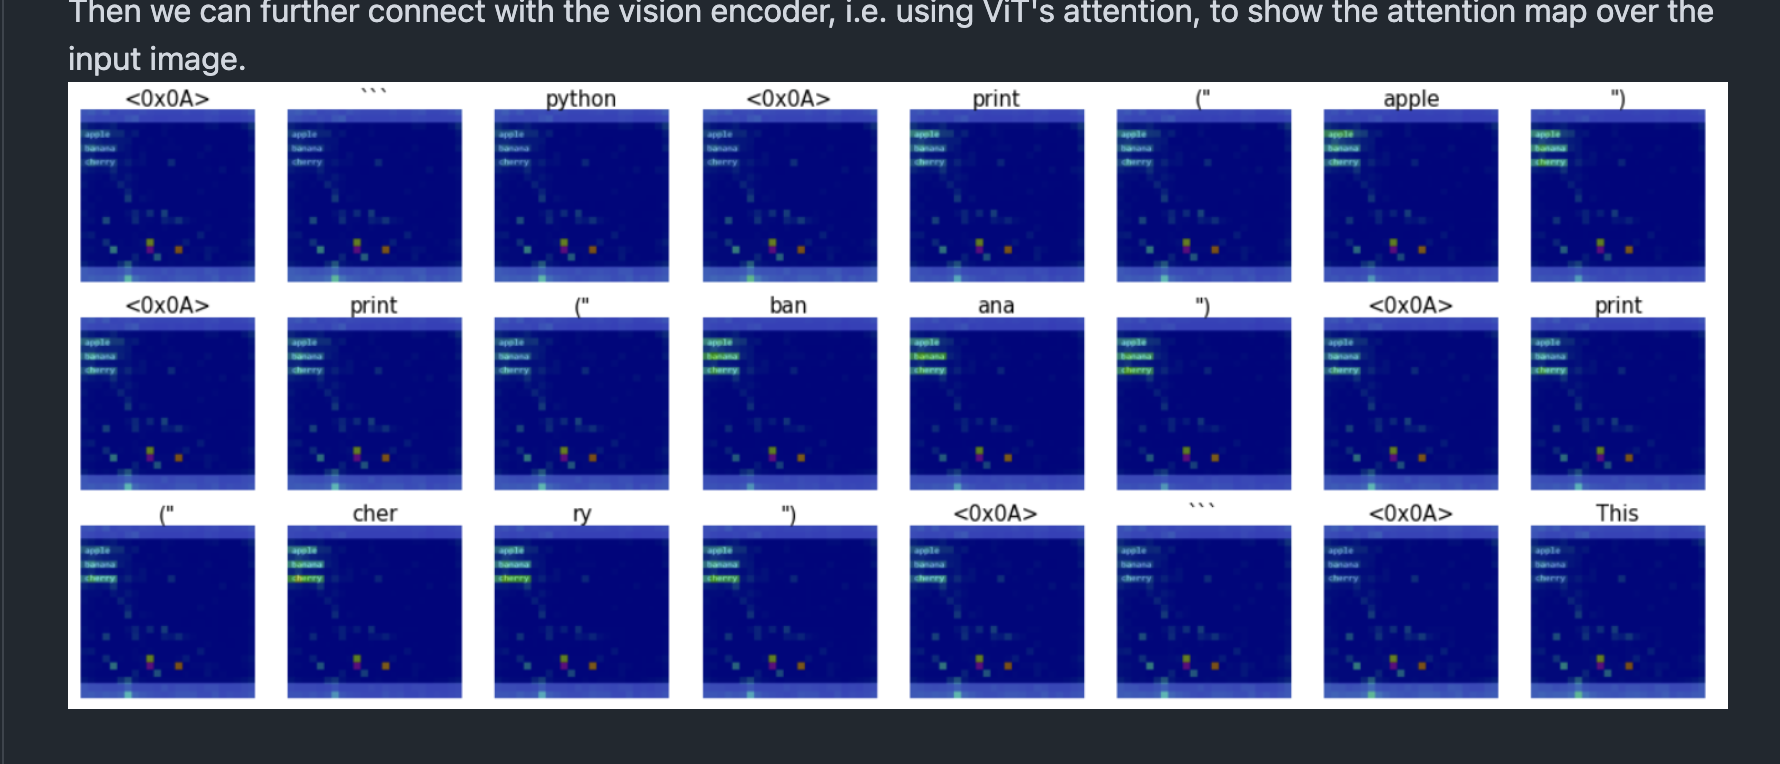
\includegraphics[width=\linewidth]{Screenshot 2025-01-22 at 5.46.55 PM.png}
         \label{fig:1a}
     \end{subfigure}
     \begin{subfigure}{0.45\textwidth}
         \centering
         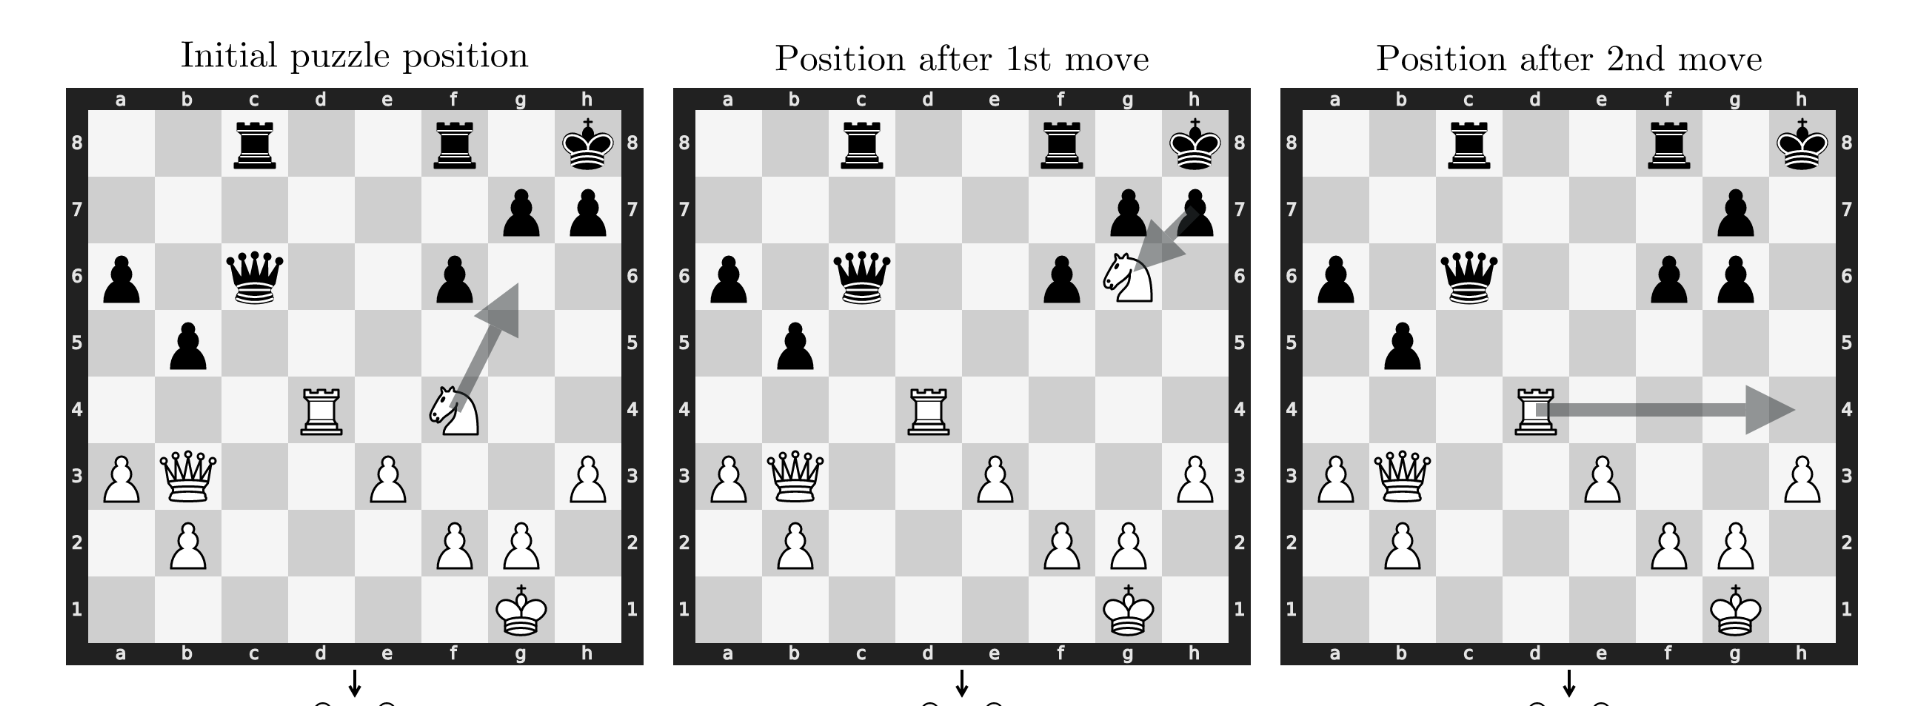
\includegraphics[width=\linewidth]{Screenshot 2025-01-22 at 5.50.06 PM.png}
         \label{fig:1b}
     \end{subfigure}
     \caption{Attention Visualization of board from decision tokens with different instruction on a position}
     \label{fig:1}
\end{figure}

\begin{figure}[!h]
    \centering
    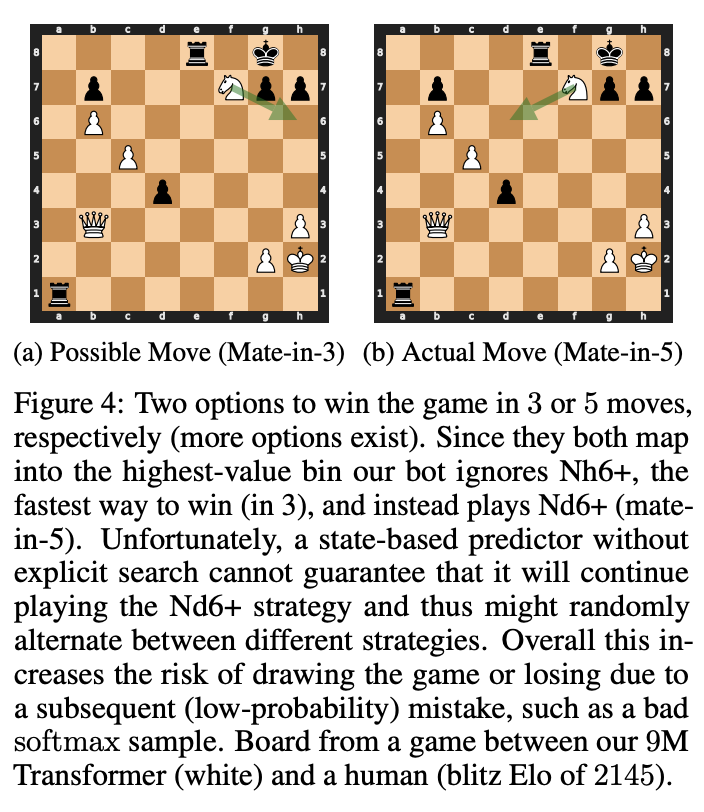
\includegraphics[width=\linewidth]{Screenshot 2025-01-22 at 5.39.44 PM.png}
    \caption{Move by move comparison on different BCL cases (Elo, DeltaElo, Time, Format)}
    \label{fig:enter-label}
\end{figure}

\subsubsection{Commentary}
We collect data of commentary on chess games from a famous Youtube channel called Agadmator aka Antonio Radić. On his channel, Radić reviews recent tournament games from top players, historical matches, and chess compositions. Almost all of Radić's videos follow the same format: a detailed analysis of one chess game. We extract paired commentary from the transcripts by aligning video clips with natural language transcripts based on timestamps.
\end{comment}